\documentclass[book,14pt,oneside,openany]{memoir}
\usepackage{nameref}
\usepackage[utf8x]{inputenc}
\usepackage[bulgarian]{babel}
\usepackage{url}
\usepackage{lipsum}
% Според изискванията на ИИКТ-БАН не бива да има номерация на страниците в ръкописа.
\usepackage{nopageno}
\usepackage{shorttoc}
\usepackage{graphicx}
% Директория в която се намират изображенията.
\graphicspath{{images/}}
\usepackage{array}
\usepackage{imakeidx}
% Добавя възможност за сензитивни хипер-връзки в самия документ.
% \usepackage{hyperref}
\usepackage{placeins}

% Заглавие на книгата.
\title{Научни изчисления с Java и Android}

% Имена на авторите.
\author{Тодор Балабанов, Илиян Занкински, Петър Томов}

% Автоматично създаване на азбучен указател.
\makeindex[columns=1, title=Азбучен указател, intoc]

\begin{document}

\maketitle

% Заглавната страница не е с оформлението на останалата част от документа (няма номерация).
\thispagestyle{empty}

% Тук стои таблицата със съдържанието, което се генерира от названието на главите.
\newpage
\shorttoc{Теми}{0}

% Тук стои таблицата със съдържанието, което се генерира от названието на главите и названието на секциите в тях.
\newpage
\tableofcontents

% По този начин номерацията на подточките е с арабски цифри.
\renewcommand\thesection{\thechapter.\arabic{section}}
\renewcommand\thesubsection{\thesection.\arabic{subsection}}

\newpage
\addcontentsline{toc}{chapter}{Предговор}
\chapter*{Предговор}

Това учебно помагало е предназначено за ученици и студенти, които биха искали да се запознаят с възможностите за реализиране на изчисления в разпределена среда\index{изчисления в разпределена среда} с използването на програмния език Java и мобилната платформа Android.

В съвременното ни ежедневие ние все по-често сме заобиколени от мобилни изчислителни устройства. Най-често това са мобилни телефони, таблети, часовници или други форми на wearables (миниатюрна електроника под формата на модни аксесоари или части от дрехи). До преди десетилетие този вид мобилни устройства бяха рядкост, а изчислителните им възможности бяха изключително ограничени. Тези два факта не позволяваха мобилните устройства да бъдат използвани за нещо повече освен основния принцип на употреба за който са създадени. С развитието на микроелектрониката и миниатюризацията на компонентите съставящи мобилните устройства техните възможности значително нараснаха за последното десетилетие. Това позволява върху този вид устройства да се извършват и допълнителни задачи, които не са били предвидени при първоначалното им проектиране. Паралелно с развитието на мобилните технологии бурен подем претърпяха и възможностите за мобилна комуникация като GSM, 3G, 4G, Wi-Fi, Bluetooth, NFC и други. Комбинацията между относително мощни мобилни изчислителни устройства и добре развита комуникационна среда открива безгранични възможности за приложение на мобилните устройства при извършването на допълнителни изчисления, в разпределена среда\index{изчисления в разпределена среда}. 

В настоящето учебно помагало ще запознаем читателите с интересните възможности, които предлагат съвременните Android мобилни устройства\index{мобилни устройства}, за постигането на резултати в научни изчислителни задачи, разпределяйки изчисленията върху физически отдалечени едно от друго устройства. Изложението на материала е организирано в следните глави. 

Глава 1 - \nameref{chapter01}: Дава кратко описание на идеята за научни изследвания и по какъв начин те могат да се впишат в ежедневния живот и използването на „умни“ мобилни устройства.

Глава 2 - \nameref{chapter02}: Представят се някои от популярните евристични подходи за решаване на сложни изчислителни задачи. Обяснява се и разликата между точните числени методи и приближените изчисления. По-сериозно внимание се отделя за генетичните алгоритми и изкуствените невронни мрежи, тъй като те са в основата на разработваната система. 

Глава 3 - \nameref{chapter03}: Излагат се различни аргументи за изготвянето на една софтуерна архитектура и се дават насоки за реалната разработка на един софтуерен проект. Изборът за архитектура на системата е насочен към трислойните модели, както в контекста на клиент-сървър система, така и в контекста на локално мобилно приложение, което се състои от потребителски интерфейс, работна логика и локална база данни. 

Глава 4 - \nameref{chapter04}: Детайлно се представя процеса по създаването на едно мобилно приложение което има за основна задача извършване на изчисления във фонов режим, чрез използване на възможностите които Android операционната система дава. Това включва приложение за активен тапет, екран за настройки и група класове за вътрешно представяне на информацията. 

Глава 5 - \nameref{chapter05}: Показва реализацията на отдалечената част от системата, а именно уеб базиран сървър с релационна база данни. За съхраняването на суровата информация за валутните котировки и параметрите на изкуствените невронни мрежи е представено MySQL базирано решение под формата на релационна база данни. За обмен на информацията между отдалечената база данни и мобилните приложения е представено PHP базирано решение. 

Глава 6 - \nameref{chapter06}: Набляга на комуникацията между отдалечения сървър и локалните клиенти, изпълнявани върху мобилни устройства. Тъй като от страната на сървъра и избрано уеб базирано решение, то в основата на комуникацията е заложен HTTP протокола и неговите възможности да предава JSON пакетирани съобщения. 

Глава 7 - \nameref{chapter07}: Разглежда обучението на изкуствени невронни мрежи, което е свързано с намиране на такива оптимални стойности за теглата, че мрежата максимално добре да изпълнява задачата за която е предназначена. При липсата на обратни връзки се използва обратно разпространение на грешката, а при наличието на обратни връзки генетични алгоритми. 

\newpage
\chapter{Научни изчисления}
\label{chapter01}

Още в зората на съвременната изчислителна техника най-съществените пресмятания са били с научна насоченост и военно дело. Този факт не се е променил значително за последните десетилетия. Дори в наши дни най-сериозните изчислителни ресурси са насочени в областта на науката. Това дава основание да обърнем значително внимание на начините по които можем да изпълняваме научни изчисления дори и върху изчислителни устройства, чието основно предназначение не е с научна цел. 

\section{Последователно програмиране}

При последователното програмиране\index{последователното програмиране} всяка изчислителна инструкция следва всички предходни. В зората на изчислителната техника пресмятанията са извършвани по този начин. Дори в наши дни значителна част от алгоритмите се изпълняват само последователно, тъй като входните данни за всяка инструкция зависят от изходните данни на предходните инструкции. Последователните алгоритми не подлежат на декомпозиране и поради тази причина са неприложими за паралелни пресмятания. 

\begin{figure}[h]
  \centering
  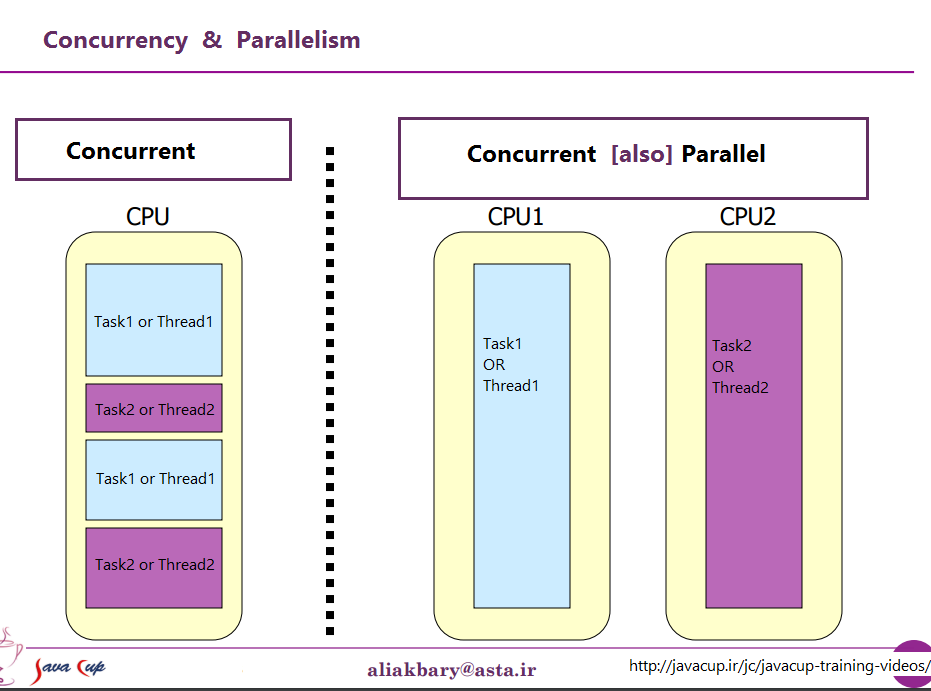
\includegraphics[width=1.0\linewidth]{pic0001}
  \caption{Сравнение между последователни пресмятания и паралелни пресмятания.}
\label{fig:pic0001}
\end{figure}

\section{Паралелно програмиране}

При паралелното програмиране основно се говоир за две разновидности - конкурентни пресмятания\index{конкурентни пресмятания} и паралелни пресмятания\index{паралелни пресмятания}. Конкурентните пресмятания са в среда където група от задачи могат да се пресметнат едновременно, без да има значение от реда на пресмятане. В същото време, паралелните пресмятания се отнасят за едновременно пресмятане на отделни задачи, върху отделни процесори. В този контекст всички паралелни пресмятания са конкурентни пресмятания, но не и обратното (Фиг. \ref{fig:pic0001}). 

\begin{figure}[h]
  \centering
  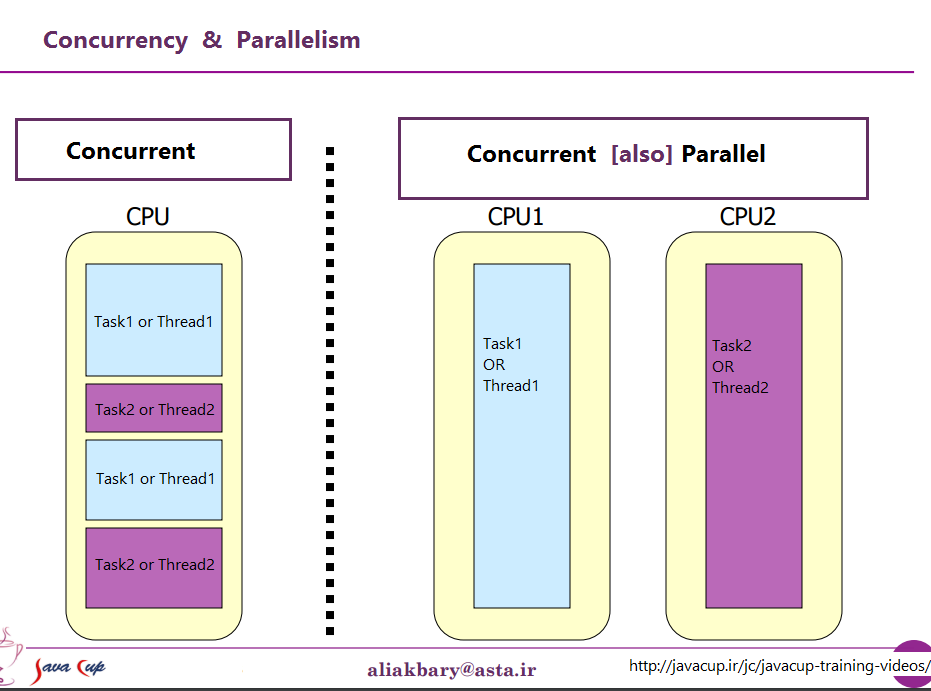
\includegraphics[width=1.0\linewidth]{pic0002}
  \caption{Сравнение между конкуретни пресмятания и паралелни пресмятания.}
\label{fig:pic0002}
\end{figure}

\section{Супер компютри и грид изчисления}

Когато паралелните алгоритми се изпълняват на изчислителни машини с множество процесори и/или множество ядра на процесорите, този вид изчисления се определят като супер компютърни\index{супер компютърни изчисления} (supercomputing). Същественото при този вид пресмятания е, че се използва много бърз вътрешна шина (понякога оптична) и споделена оперативна памет. За разлика от супер компютрите\index{супер компютърни изчисления} грид изчисленията\index{грид изчисленията} се осъществяват на множество машини, свързани в обща мрежа, но работещи автономно, без да споделят обща памет. При грид системите отделните изчислителни машини могат да са териториално отдалечени една от друга. Съществено е да се отбележи, че и при супер компютрите\index{супер компютърни изчисления} собственикът на системата има пълен контрол над нея. Това може малко да се различава за грид системите, ако към грида са включени компютри под чужд контрол. 

\section{Изчисления в разпределена среда}

Преходът от грид системите към системи за изчисления в разпределена среда\index{изчисления в разпределена среда} се състои в това, че изчислителните машини в разпределената среда са абсолютно автономни. Тези машини не споделят общи ресурси, като процесор или оперативна памет. Много характерно е в разпределената среда контролът над изчислителните машини да не е от страната на организиращия изчисленията. Това води до два основни проблема - ненадеждна (често и твърде бавна) комуникация, липса на гаранция за коректност на пресмятанията (манипулации от страна на притежаващия изчислителните ресурси). Също така, при грид системите често се наблюдава хомогенност на изчислителните ресурси по отношение на хардуерни конфигурации и операционна система, докато в разпределената среда изчислителните машини са основно хетерогенни, което може да води до големи разлики в хардуера и операционните системи. 

\section{Дарена изчислителна мощност}

За решаването на някои по-мащабни научни проблеми изчислителната мощност и/или финансовите ресурси често са недостатъчни. В такива ситуации не малко научни институции прибягват до така наречените дарени изчислителни ресурси\index{дарени изчислителни ресурси} в разпределена среда\index{изчисления в разпределена среда}. Един от най-изчерпателните списъци с проекти от този вид може да бъде открит в уеб сайта Distributed Computing Info \cite{dcinfo}. Съществено е да се отбележи, че не всеки изчислителен проблем е подходящ за решение в разпределена среда\index{изчисления в разпределена среда} с дарена изчислителна мощ. На първо място проблемът трябва да подлежи на декомпозиране, така че отделни части от него да се пресмятат едновременно. Второто важно нещо е да не е от съществено значение в кой момент от времето и в какъв ред ще бъдат получени пресметнатите резултати. И третото съществено нещо е да е наличен механизъм за проверка на достоверността от пресмятанията, тъй като изчисленията се извършват на машини с различна хардуерна конфигурация и различни операционни системи, а освен това са възможни манипулации от страна на хората притежаващи тези машини. Най-известният проект за дарена изчислителна мощ е SETI@home \cite{shuch}, като неговата цел е да търси сигнали от космоса, които да са създадени от интелигентни форми наживот.

Когато изчисленията се извършват на мобилни устройства, то разпределената среда се превръща в мобилна среда за разпределени изчисления\index{мобилна среда за разпределени изчисления}. В останалата част от това учебно помагало ще бъде представено точно изграждането на система за извършване на разпределени изчисления върху мобилни устройства. 

\newpage
\chapter{Евристични алгоритми}
\label{chapter02}

Евристичните алгоритми са подход за решаване на изчислителни проблеми, основаващи се на опита и интуицията. Този вид алгоритми не гарантират оптимално решение за поставената задача. Евристичните алгоритми намират широко приложение при задачи, които трудно се поддават на точни числени методи или аналитични решения. Макар и да не могат да предложат оптимално решение, евристичните алгоритми\index{евристични алгоритми} често водят до достатъчно приемливи в практиката, близки до оптималното решения. Благодарение на своята не детерминистична природа, евристичните алгоритми\index{евристични алгоритми} са изключително подходящи за реализация в супер компютърни изчисления\index{супер компютърни изчисления}. Две изключително популярни евристики\index{евристики} са изкуствените невронни мрежи\index{изкуствени невронни мрежи} и генетичните алгоритми\index{генетични алгоритми}. Те са обект на особена популярност през последните две десетилетия и това дава основание да бъдат заложени в основното изложение на настоящото учебно помагало. Сами по себе си евристиките са безполезни, ако не бъдат приложени върху достатъчно сложна изчислителна задача. Точно такава сложност предлагат задачите за прогнозиране. Прогнозирането е залегнало в множество дейности от човешкото ежедневие, като започнем от средните дневни температури и стигнем до потреблението на определени стоки и услуги. Под една или друга форма почти всяка човешка дейност бива остойностена в термините на финансовите ресурси. Този факт дава основание да бъдат разгледани точно прогнози за промяната в цените на различни финансови инструменти. Отчитането на промяната в цената, на определени интервали (равни или неравни), води до представяне на информацията във времеви ред\index{времеви редове}. При времевите редове\index{времеви редове} по абсцисната ос се означава времето, а по ординатната ос стойността на измерваната величина (в конкретния случай цената).

\section{Финансови времеви редове}

Времевите редове\index{времеви редове} са серия от замервания извършени в последователен ред във времето. Практически се получава последователност от дискретни стойности. Времевите редове могат да са съставени от стойности на равни интервали или стойности на произволни интервали. Често в практиката се случва да има липсващи замервания, което води до определени усложнения при анализирането. При финансовите времеви редове основно се използват равни интервали на отчитане и рядко има липсващи стойности при отчитането. Всяко едно отчитане при финансовите времеви редове се отличава с група стойности, характеризиращи времевия интервал за който се отнася, а именно – начална стойност за интервала, най-висока постигната стойност за интервала, най-ниска стойност постигната за интервала и крайна стройност за интервала. 

\begin{figure}[h]
  \centering
  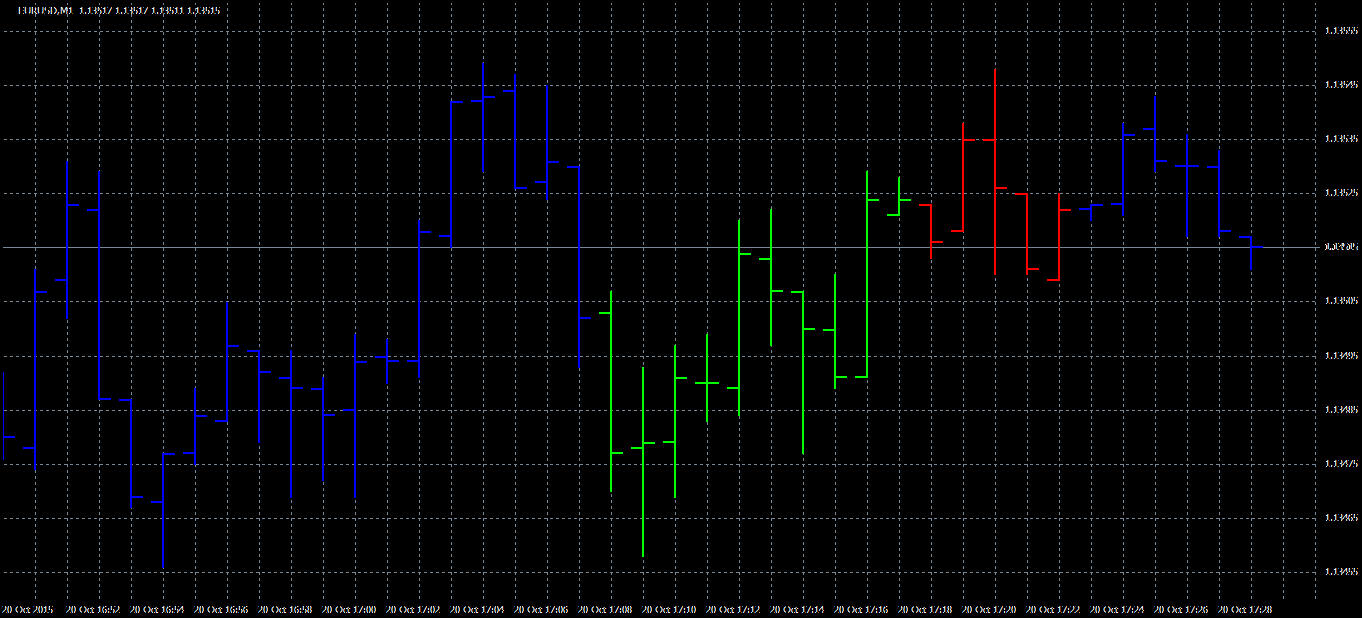
\includegraphics[width=1.0\linewidth]{pic0003}
  \caption{Отношението евро/долар в рамките на един час.}
\label{fig:pic0003}
\end{figure}

На Фиг. \ref{fig:pic0003} тази информация се обозначава с вертикални черти, като долният край на вертикалната черта символизира най-ниското ниво, горният край най-високото ниво, а двете странични чертички маркират нивото на отваряне (отляво) и нивото на затваряне (от дясно). Анализирането на времевите редове\index{времеви редове} може да предостави съществена информация за лицата вземащи решения. Когато става въпрос за времеви редове във финансовата област основна цел на анализа е предлагането на прогноза. Една от най-често използваните форми на анализ е напасването на крива (curve fitting). От математическа гледна точка задачата представлява построяване на крива която да премине максимално близо до предварително определени точки. От математиката е добре известно, че през краен брой точки могат да се построят безкрайно на брой преминаващи криви. За да има смисъл от напасването кривата трябва да притежава определени свойства, като изглаждане, добра интерполация и екстраполация. 

Условното разделяне на финансовия времеви ред\index{финансови времеви редове} на две половини (минало и бъдеще) дава изключително добра възможност за представяне на задачата по прогнозиране в термините на изкуствените невронни мрежи\index{изкуствени невронни мрежи}. Мащабираната информация от миналия период (зелено на графиката) се подава към входния слой на изкуствената невронна мрежа, а прогнозата се получава в изходния слой на изкуствената невронна мрежа и се подлага да обратно мащабиране (червеното на графиката). Така декомпозиран времевият ред\index{времеви редове} се използва при фазата за обучение на изкуствената невронна мрежа. За работната фаза на мрежата за прогноза на изкуствената невронна мрежа се подават последните измерени стойности, без да има яснота какви са бъдещите измервания. 

\section{Изкуствени невронни мрежи}

Изкуствените невронни мрежи\index{изкуствени невронни мрежи} са се появили в следствие на опитите за изграждане на математически модел за биологичните нервни системи. Този вид системи се научават (прогресивно подобряват възможностите си) с изследването на примерни данни. Приложението им е основно при задачи за които традиционните алгоритми не дават приемливи резултати. Най-широко приложение изкуствените невронни мрежи намират в задачи за класификация. Когато става въпрос за финансови времеви редове са възможни две събития – повишаване на стойността или понижаване на стойността. Според информацията в отминалите периоди време, изкуствената невронна мрежа\index{изкуствени невронни мрежи} може да раздели данните в два основни класа – данни показващи промяна към повишение или данни показващи промяна към понижение. 

\begin{figure}[h]
  \centering
  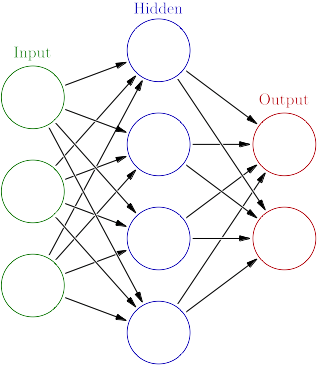
\includegraphics[height=0.25\pdfpageheight]{pic0004}
  \caption{Трислойна изкуствена невронна мрежа.}
\label{fig:pic0004}
\end{figure}

Структурата на класическите изкуствени невронни мрежи\index{изкуствени невронни мрежи} се състои от възли, наречени изкуствени неврони и връзки, наречени тегла (Фиг. \ref{fig:pic0004}). Връзките между невроните служат за предаване на сигнал от един неврон към друг. Невроните които получават сигнали ги обработват по предварително заложено правило и след това могат на свой ред да ги разпространят към други неврони. В класическият случай невроните имат стойност (обикновено това е реално число). Връзките между невроните също са представени със стойност и според правилото за обучение точно тази стойност подлежи на промяна, така че мрежата да заучава необходимата информация. При най-използваните изкуствени невронни мрежи\index{изкуствени невронни мрежи} невроните са организирани в слоеве. Сигналите при този вид мрежи се разпространяват от входния слой към изходния слой, като преминават междинните слоеве. Това разпространение на сигналите се нарича пас в права посока и е характерно за режима на експлоатация. Освен режим на употреба изкуствените невронни мрежи\index{изкуствени невронни мрежи} работят и във втори режим, наречен режим на обучение. За последните няколко десетилетия са предложени множество начини за обучение на изкуствени невронни мрежи, като най-значими резултати се получават при използването на алгоритъма за обратно разпространение на грешката\index{обратно разпространение на грешката}. Обратното разпространение на грешката представлява точен числен метод от групата на градиентните методи, който разчита на грешката, която мрежата допуска при изпълнението на обучаващите примери. Тази допусната грешка се установява в изходния слой и след това се разпространява обратно по предходните слоеве, от където идва и названието на метода. 

Според своята линейна природа, обратното разпространение на грешката\index{обратно разпространение на грешката} трудно се поддава на реализация в термините на паралелното програмиране. Ако се погледне на теглата в една изкуствена невронна мрежа като на многомерно безкрайно пространство от реални числа, то намирането на стойности за теглата е математическа оптимизационна задача. Точните числени методи дават добри резултати при пространства с относително малка размерност, но срещат сериозни затруднения при по-големите размерности. Точно противоположно на точните числени методи, евристичните алгоритми предлагат приемливи решения, в разумно време. Предимство е не само ефективността, но и значително по-големите възможности евристичните алгоритми да се реализират в термините на паралелното програмиране. 

Класическите неврони реализират трансферна функция и активационна функция. Най-често използваната трансферна функция е линейната, която представлява сума от умножение на входните сигнали по теглата, които ги доставят. Най-често използваните активационни функции са сигмоидната функция и хиперболичния тангенс. Активационната функция има основна роля за нормиране на изходния сигнал. Тази нормализация е необходима тъй като за трансферната функция, при различните неврони, постъпват различен брой сигнали и без нормализация това би направило изходните сигнали несъизмерими. При градиентните точни числени методи има изискване активационната функция да бъде диференцируема, нещо което не е необходимо при евристичните алгоритми. Често използваната линейна трансферна функция има нужда от използване на допълнително събираемо наречено „отместване“ (bias). От формална гледна точка, отместването може да се интерпретира като тегло свързващо неврона с друг неврон, който емитира единичен сигнал. В практиката за всеки слой е прието да се отделя неврон емитиращ единичен сигнал. Само в изходния слой е безсмислено такъв неврон да има, тъй като той не получава входни сигнали, а емитирането на постоянна единица в изхода не носи смислена информация за функционирането на мрежата. 

От математическа гледна точка класическите невронни мрежи могат да се представят с вектор (стойностите на невроните) и матрица (стойностите на теглата между невроните). Разпространението на сигналите от входа към изхода в този случай би бил умножение на вектор с число. В настоящото учебно помагало на класическа трислойна мрежа ще се подават мащабираните стойности от изминалите времеви периоди, а на изхода ще се очаква прогнозна стойност за бъдещи времеви интервали. Тази концепция е малко по-сложна от идеята за проста квалификация от вида повишение/понижение, но е значително по-информативна, защото се очаква да дава представа за един по-дълъг времеви интервал в бъдещето. След успешно прогнозиране в коя посока ще се промени цената от съществено значение става и въпросът колко дълго ще продължи този спад/повишение. 

\section{Генетични алгоритми}

Генетичните алгоритми представляват глобална оптимизационна евристика\index{глобална оптимизационна евристика} вдъхновена от идеите за биологичната еволюция. Генетичните алгоритми са подмножество на класовете популационни алгоритми и еволюционни алгоритми. Основното си приложение генетичните алгоритми\index{генетични алгоритми} намират при задачи с голяма по размерност пространство на решенията. Често при такива задачи класическите точни числени методи не могат да предложат решение в приемливо време. За да се приложи генетичен алгоритъм решението на съответната задача трябва да се представи под формата на хромозома (индивид) в обща популация от решения. След това, чрез прилагане на основните операции по селекция\index{селекция в генетичен алгоритъм}, кръстосване\index{кръстосване в генетичен алгоритъм} и мутация\index{мутация в генетичен алгоритъм} (Фиг. \ref{fig:pic0005}), отделните индивиди (решения) следва да бъдат подобрявани.

\begin{figure}[h]
  \centering
  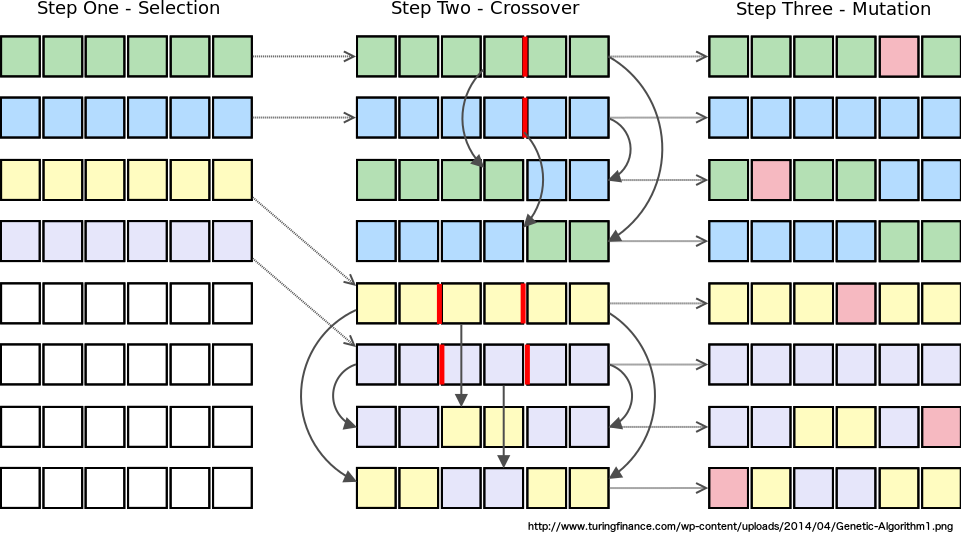
\includegraphics[width=1.0\linewidth]{pic0005}
  \caption{Трите основни операции в генетичните алгоритми.}
\label{fig:pic0005}
\end{figure}

При класическия процес оптимизацията започва от случайно генерирани индивиди, Това не е задължително особено когато става въпрос за хибридни реализации в които генетичният алгоритъм е поддържаща оптимизация. При такива ситуации началната популация може да бъде получена в резултат на друга оптимизация или в резултат на човешка подредба. След началната фаза оптимизацията протича итеративно и приключва според предварително определени критерии за край. Най-често се използва предварително дефиниран брой поколения или брой поколения които не водят до подобрение в намерените решения, но също така е възможно да се дефинира и интервал астрономическо време. 

От основна важност за успешната работа с генетичните алгоритми\index{генетични алгоритми} е определянето на целева функция (жизнена функция\index{жизнена функция} на индивида) която еднозначно да определя качеството на полученото решение. На база различната жизненост която индивидите в популацията притежават се взема стохастично решение кои индивиди да участват в създаването на бъдещото поколение и кои не. В множество реализации на генетични алгоритми се прилага правило на елита, така че най-доброто открито решение да достигне края на оптимизационния процес. В същото време правилото на елита крие риск от израждане на популацията, така че всичките решения в нея да клонят към съхранения елит.  

Фактът, че генетичните алгоритми са организирани на принципа на популацията от индивиди ясно подсказва идеалната възможност оптимизационния процес да се организира не в една глобална популация, а в множество различни локални популации които да съществуват на различни изчислителни машини. Това от своя страна би дало възможност за реализиране на миграционни процеси, точно както това се наблюдава при естествените биологични видове. 

\section{Прогнозиране в разпределена среда}

Гъвкавите възможности на изкуствените невронни мрежи\index{изкуствени невронни мрежи} да изграждат функционална зависимост между входни и изходни данни ги прави идеален кандидат за прогнозираща система. Ако се приеме, че измерените стойности във времевия ред са точки в двуизмерно пространство, то задачата за прогнозиране може да се представи като задача за прекарване на крива през N точки (curve fitting). Ако образно се оприличи изкуствената невронна мрежа на полином, то теглата й биха представлявали коефициенти в полинома. Стойностите които изкуствената невронна мрежа\index{изкуствени невронни мрежи} генерира на изхода си за бъдещи моменти от времето представляват своеобразна екстраполация\index{екстраполация} според апроксимираната крива. Тъй като класическите многослойни невронни мрежи работят с входни сигнали между 0.0 и 1.0 или -1.0 и +1.0, то информацията от времевия ред трябва да бъде мащабирана в съответния работен интервал на мрежата. Стойностите на времевия ред условно се разделят на минали (зелените Фиг. \ref{fig:pic0003}) и бъдещи (червените Фиг. \ref{fig:pic0003}). Изходната (прогнозна) информация на изкуствената невронна мрежа след това се мащабира обратно към оригиналните интервали на времевия ред.

\begin{figure}[h]
  \centering
  
\includegraphics[width=1.0\linewidth]{pic0006}
  \caption{Продуктовата линия TradingSolutions използваща изкуствени невронни мрежи и генетични алгоритми за прогнозиране на Forex финансови инструменти.}
\label{fig:pic0006}
\end{figure}

От чисто практическа гледна точка, използването на изкуствени невронни мрежи и генетични алгоритми се е доказало като удачен подхода за прогнозиране на финансови инструменти, което ясно се вижда в продуктовата линия на TradingSolutions (Фиг. \ref{fig:pic0006}). Почти петнадесет години продуктовата линия на TradingSolutions доставяше системи за подпомагане вземането на решения\index{системи за подпомагане вземането на решения}. По настояще тази продуктова линия е придобита от компанията nDimensional, Inc.

\begin{figure}[h]
  \centering
  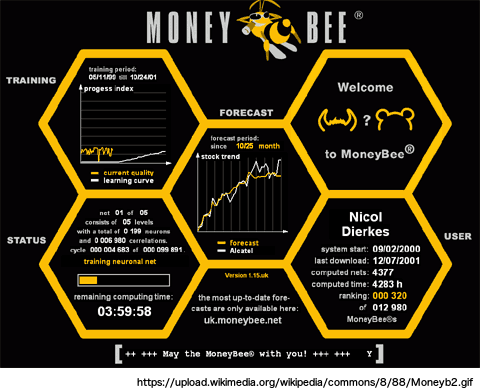
\includegraphics[height=0.4\pdfpageheight]{pic0007}
  \caption{Системата MoneyBee за финансово прогнозиране в разпределена среда.}
\label{fig:pic0007}
\end{figure}

Възможността да се прогнозират цените на финансови инструменти винаги е привличала не само индустрията, но и научните среди. Едно от най-забележителните постижения в тази насока е проектът MoneyBee (Фиг. \ref{fig:pic0007}). Макар и вече да не съществува, този проект предлагаше възможност за изчисляване на прогнози с помощта на дарена изчислителна мощност\index{дарени изчислителни ресурси} в разпределена среда\index{изчисления в разпределена среда} \cite{bohn}. Същинските прогнози се пресмятаха, с помощта на изкуствени невронни мрежи, върху изчислителните машини на потребителите в периоди когато натоварването на машините е ниско и се активира програмата за защита на монитора (screensaver). Преди масовото навлизане на мобилните устройства честа практика при проектите за дарена изчислителна мощност, с цел пресмятане в разпределена среда\index{изчисления в разпределена среда}, основен подход бе извършване на пресмятанията в специално създадена за целта програма за предпазване на монитора. След навлизането на катодно лъчевите тръби при настолните компютри се появява ефект от увреждане на монитора, ако върху него продължително се визуализира статична картина. Решаването на този проблем се оказва най-удачно с помощта на операционната система, която да установи период в който потребителя не използва изчислителната машина и да активира софтуерна програма за предпазване на монитора. Развитието на мониторите с течни кристали постепенно изведе от употреба мониторите с катодно-лъчеви тръби и използването на програми за предпазване на монитора изгуби своето първоначално предназначение. Въпреки това този вид софтуерни решения останаха в употреба и основно служат за повишаване на информационната сигурност, като не само дават естетическа визуализация, но и привеждат работната сесия на потребителя в заключено състояние, което възпрепятства използването на компютърната система от неауторизирани потребители. Наличието на изчислителни ресурси, които са налични, но неефективно използвани дава основание на множество учени да разработят системи за отдалечено пресмятане в разпределена среда\index{изчисления в разпределена среда}, точно под формата на програми за предпазване на монитора, които да се възползват от дарените потребителски, изчислителни ресурси. 

\section{Фонови пресмятания върху мобилни устройства}

Съществува концептуална разлика в начина по който потребителите използват настолните си компютри и мобилните устройства. На първо място, настолният компютър бива пускан и спиран според нуждите на потребителя, докато най-често мобилните устройства са в непрекъснат режим на употреба. Това води до основната разлика, че мобилните устройства не изпадат в режим на занижена употреба, но също така имат режими за употреба при изключителна важност (примерно телефонно обаждане с висок приоритет). Втората фундаментална разлика се състои във факта, че основен похват за пестене на електрическа енергия, доставяна предимно от батерии при мобилните устройства, е динамичното изгасяне на екрана. Тази стратегия за пестене на енергия кардинално отменя концепцията за програма предпазваща монитора. За да се реализира ефективно система за разпределени пресмятания върху мобилни устройства е много по-удачно да се използва технологията за активен тапет, отколкото да се залага да идеята за програма предпазваща монитора. Точно тази идея е развита в настоящото учебно помагало. 

\newpage
\chapter{Софтуерна архитектура}
\label{chapter03}

Разработката на софтуер е в областта на инженерните науки, тъй като продуктът се създава по принципите за изграждане на конструкции (в случая софтуерни). При стартирането на нов софтуерен проект трябва да се вземат редица решения, според заданието на потребителя. В настоящата разработка целта е софтуерно решение което извършва изчисления от страната на клиентски мобилни устройства. Задачите за пресмятане се възлагат от сървър и получените пресметнати резултати се получават обратно на същата машина. От страната на клиента се получават стойности за цена на валути под формата на времеви ред. Сървърът изпраща на клиента също информацията за топология на изкуствена невронна мрежа. Клиента от своя страна използва котировките на валутите и информацията за изкуствената невронна мрежа за да извършва пресмятанията необходими за обучението на изкуствената невронна мрежа. Процесът по обучението на изкуствената неверонна мрежа\index{изкуствени невронни мрежи} се извършва с помощта на генетични алгоритми\index{генетични алгоритми}, които имат за цел търсене на възможно по-оптимални стойности за теглата на мрежата. Клиентското приложение също поема отговорностите за визуализация на процеса по обучение и визуализация на постигнатите прогнози. Така представена системата съвсем естествено води към избора на „клиент-сървър“ софтуерна архитектура. 

\section{Избор на развойни средства}

В съвременната софтуерна индустрия има голям избор от развойни средства\index{развойни средства} за различните нужди на софтуерните разработчици. Една част от развойните средства са комерсиални, докато друга част са инструменти с отворен код. В настоящата разработка акцентът основно пада върху развойни средства с отворен код, тъй като минимизирането на разходите за производство е основен стремеж с цел постигане на икономическа ефективност. Изборът на развойни инструменти е задача от областта на мококритериалния анализ и основно се характеризира с наличието на множество критерии, които често са противоречиви. 

\subsection{От страна на сървъра}

За уеб базирани сървър решения най-популярни са технологиите JSP, ASP, PHP и Node.js. Тъй като ASP е комерсиална технология на фирмата Microsoft тя не представлява интерес за настоящата разработка. JSP e технология на фирмата Oracle която е с отворен код и дава възможност за изграждане на стабилни корпоративни решения. Недостатък на JSP е нуждата от по-сериозни софтуерни и хардуерни ресурси по отношение на хостинга. Node.js е технология, която набира все по-голяма популярност, но все още не е достигнала достатъчно ниво на „зрялост“, като същевременно също изисква повече софтуерни и хардуерни ресурси от страна на хостинга. По отношение на PHP, технологията е с тясно предназначение и има едно от най-високите нива на „зрялост“. В същото време разходите за хостинг при PHP са едни от най-ниските, което прави избора на тази технология изключително икономически ефективно. Задачата на уеб базираната сървър технология е да служи като посредник между мрежата и системата за управление на бази от данните. От страна на сървъра най-рационално е данните да се съхраняват в релационна база данни. Съществуват множество решения които да бъдат приложени в тази част на системата, като най-популярните са: Oracle, MS SQL Server, PostgreSQL и MySQL. Oracle намира своето приложение в корпоративния сегмент и е свързан със значителни финансови разходи, което го прави неприемлив за настоящата разработка. MS SQL Server е система алтернативна на Oracle в корпоративния сегмент и също е свързана със значителни финансови разходи. PostgreSQL е система с отворен код, която е съизмерима с технологичните възможности на Oracle и е потенциално добър кандидат за ниско бюджетни разработки. В настоящата разработка PostgreSQL е избегнат поради своята ненужна сложност, при едно относително просто софтуерно решение. Изборът пада върху MySQL, тъй като системата е максимално опростена добре наложена сред потребителите и поддържа се от фирмата Oracle. Освен всичко изброено, MySQL има добра поддръжка при хостинг доставчиците и е икономически най-ефективният избор. 

\subsection{От страна на клиента}

При „умните“ мобилни устройства най-разпространените операционни системи са Android, iOS и Windows Phone. По настояще фирмата Microsoft преустанови развитието на своята операционна система Windows Phone, което моментално води до отхвърлянето й за настоящата разработка. Инвестицията за разработка на приложения под iOS на фирмата Apple води до отпадането на тази платформа за нуждите на настоящата разработка. Към разходите за разработка може да се добави и факта, че програмирането за iOS се извършва на два езика Objective-C и Swift, който имат относително малка популярност в Източна Европа. Най-много „умни“ мобилни устройства в световен мащаб се използват с операционната система Android. Android е с отворен код, поддържа се основно от компанията Google и позволява разработка с значително по-ниски финансови разходи, спрямо конкурентите си. Приложенията за Android основно се разработват на езика Java, който по настояще е един от най-широко използваните програмни езици и се характеризира с много висока степен на „зрялост“. 

\subsection{За комуникация между сървъра и клиента}

Съществуват множество възможности за изграждането на комуникацията между сървъра и клиента. В най-суров вид информацията може да се предава като серия байтове (plane text), което води до множество затруднения при получаването и последващата й обработка. Широко използвана алтернатива е тагиращия език XML. При този вариант информацията бива „пакетирана“ в серия от тагове, които дават определена структура и семантика. Основният замисъл при проектирането на XML е бил създаването на структурирани документи, както от хора, така и от машини. Поради тази причина XML има една по-голяма експресивност в сравнение с неговата алтернатива JSON. JSON е максимално опростен тагиращ език за структурирано представяне на информацията, който води своето начало от обектите в програмния език JavaScript. За разлика от XML, JSON има основно предназначение за обмяна на структурирана информация между машини, а не толкова между хора и машини. Поради всичко изброено, в настоящата разработка изборът пада върху JSON като основа за изграждането на комуникационния протокол между сървъра и неговите клиенти. Тъй като от страната на сървъра се предвижда уеб базирано решение, то JSON базирания протокол ще протича в комуникационни сесии на HTTP протокола. В зората на уеб страниците е разработен протокола HTTP, стъпващ на TCP/IP, за ефективно предаване на информация между уеб сървърите и уеб браузърите. HTTP протоколът е добре наложен и с добра поддръжка в световен мащаб. Една важна негова характеристика е, че при този протокол комуникацията е разделена на заявки и отговори, без да се поддържа постоянна комуникационна линия. 

\section{Компоненти на системата}

След направеният кратък обзор на технологии и развойни средства изборът е за направата на „клиент-съръвр“ система. От страна на сървъра се разполагат модули за съхранение на данните (MySQL система за управление на бази от данни) и за комуникация (PHP уеб скриптове). Уеб сървърът комуникира с клиентите на база JSON/HTTP комуникационен протокол. Android мобилни устройства правят уеб заявки, извършват изчисленията и връщат резултата до сървъра. Тъй като се разчита на дарена изчислителна мощност\index{дарени изчислителни ресурси} е нужно да се избере подходящ начин за използване на мобилното устройство, без това да нарушава основните му функции и без да пречи на потребителите. Със своята технология Active Wallpaper, Android предлага идеална възможност за цените на настоящата разработка. Активният тапет представлява изображение, което се изрисува зад всички основни графични компоненти от графичния потребителски интерфейс на Android. По-същественото е, че активния тапет е Java приложение, което работи в постоянен фонов режим и може да изпълнява определени кратки задачи, когато устройството не е високо натоварено. 

\begin{figure}[h]
  \centering
  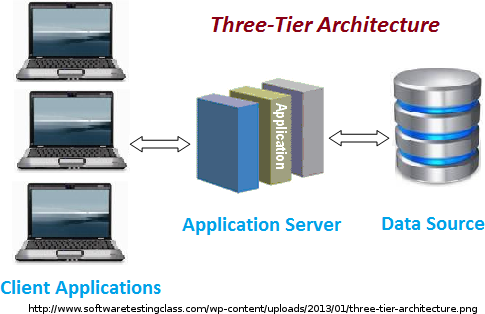
\includegraphics[height=0.25\pdfpageheight]{pic0008}
  \caption{Уеб базирана трислойна софтуерна архитектура.}
\label{fig:pic0008}
\end{figure}

При реализацията на настоящата система за изчисления в разпределена среда\index{изчисления в разпределена среда} изборът пада върху класическа трислойна софтуерна архитектура. Същият подход за три слоя се прилага и при реализацията на мобилното приложение, където SQLite локално съхранява данните над които се работи, Java обектно-ориентиран код извършва изчисленията, а Android базиран графичен потребителски интерфейс поема отговорността за визуализацията на процеса пред потребителя. 

\subsection{Подход за разработка}

\begin{figure}[h]
  \centering
  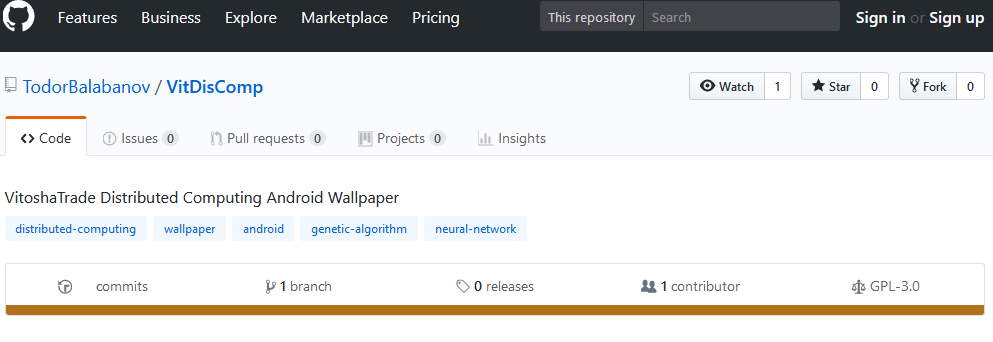
\includegraphics[width=1.0\linewidth]{pic0009}
  \caption{Подходи за софтуерна разработка.}
\label{fig:pic0009}
\end{figure}

Ако приемем, че визуализацията е най-горният слой, а базата данни най-долният слой на една трислойна софтуерна архитектура, то има два основни подхода за изработване на софтуерната система (Фиг. \ref{fig:pic0009}). При първия подход първоначално се разработва визуалния интерфейс, след това слоя на работната логика и накрая базата данни. Този подход се нарича „top-down“и е полезен когато се анализира софтуерно задание при което вече има в употреба множество хартиени документи (първоизточници на работните екрани. Този подход също е удобен при проекти с малък размер, където базата данни е относително опростена. Вторият много популярен подход е когато се започне с проектирането на базата данни, след това работната логика която обработва данните и едва накрая екраните визуализиращи информацията. Този подход се нарича „bottom-up“ и е най-подходящ когато се разработва сложно софтуерно решение, което се очаква да работи с големи обеми данни и множество различни структури на информацията. Акцентът в настоящата разработка е върху изчисленията които мобилните устройства извършват, а не толкова към създаването на голям масив от данни. Поради тази причина изборът в случая пада върху подхода „top-down“. 

\section{Лиценз и хранилище за проекта}

При съвременните софтуерни проекти с отворен код са от значение две неща – юридическият лиценз\index{софтуерни лицензи} под който съществува проекта и публичното хранилище\index{хранилища за програмен код} в което е разположен програмният текст. 

\subsection{Лиценз}

От съществено значение е изборът на правилен софтуерен лиценз, когато се разработва софтуерен проект предвиден да бъде публично достъпен. Съществуват множество възможности, като някои от най-популярните са - BSD License, MIT license, Mozilla Public License и GNU General Public License. За нуждите на настоящата разработка е предпочетен GNU General Public License v3, защото този лиценз е най-предпазващ за създателя на софтуерния продукт. В най-общи линии GPL3 позволява - комерсиална употреба, модификации, разпространение, включване в патенти и употреба за лични нужди. Лицензът съпровожда изключително ограничена отговорност за създателите на продукта и абсолютно никаква гаранция за употребата му от страна на потребителите. Лицензът също налага и серия ограничения – задължително включване на текст за авторските права на създателите, списък на извършените промени, не позволява закриване на кода и задължава всяко надграждане на продукта да бъде под същия лиценз. Със своята протекционистка природа GPL е един от лицензите дал най-силен тласък в развитието на продукти с отворен код, което е достатъчна причина да бъде избран за разработки без ясно изразена комерсиална насоченост. 

\subsection{Хранилище за програмен код}

Прието е всеки проект да има название, което особено важи в света на софтуера с отворен код. За настоящата разработка е избрано името VitDisComp. Точно това название е избрано, тъй като разработката ще се възползва от наличното сървър решение в проекта VIToshatrade \cite{vtrade} и по своята същност проектът е DIStributed COMPuting решение. 

\begin{figure}[h]
  \centering
  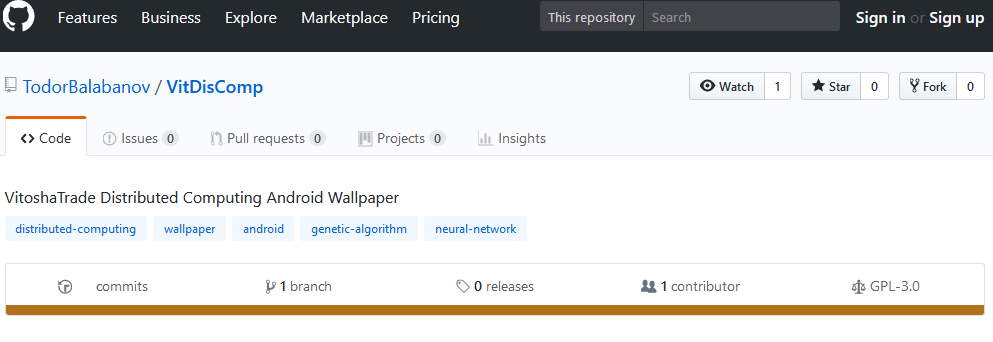
\includegraphics[width=1.0\linewidth]{pic0010}
  \caption{Публикуване на проект в GitHub.}
\label{fig:pic0010}
\end{figure}

Съществуват различни възможности за публикуване на програмния код, но една от най-популярните алтернативи е облачната услуга GitHub. Услугата GitHub (Фиг. \ref{fig:pic0010}) е базирана на системата за контрол на версиите Git и дава една от най-широките възможности за популяризиране на програмен код с отворен лиценз. 

\newpage
\chapter{Android активен тапет}
\label{chapter04}

Технологията Android Live Wallpaper предоставя анимирани възможности за визуализация под формата на виртуален тапет. По своята същина този вид приложения не се различават драстично от останалите Android  приложения и дори могат да изпълняват почти всички техни възможности. Тъй като виртуалният тапет е постоянно активен той е идеален кандидат за реализацията на пресмятания във фонов режим\index{изчисления в разпределена среда}. За създаването на активен тапет са необходими следните компоненти: 1. XML файл който описва компонентите на тапета; 2. Фонов модул (Android Service); 3. Подходящи флагове за достъп до ресурсите на устройството. 

\section{Манифест файл на мобилното приложение}

При създаването на приложения за операционната система Android е възприет подхода компонентите на мобилното приложение да бъдат описани в манифест файл (AndroidManifest.xml), с използването на XML синтаксис. 

\begin{figure}[h]
  \centering
  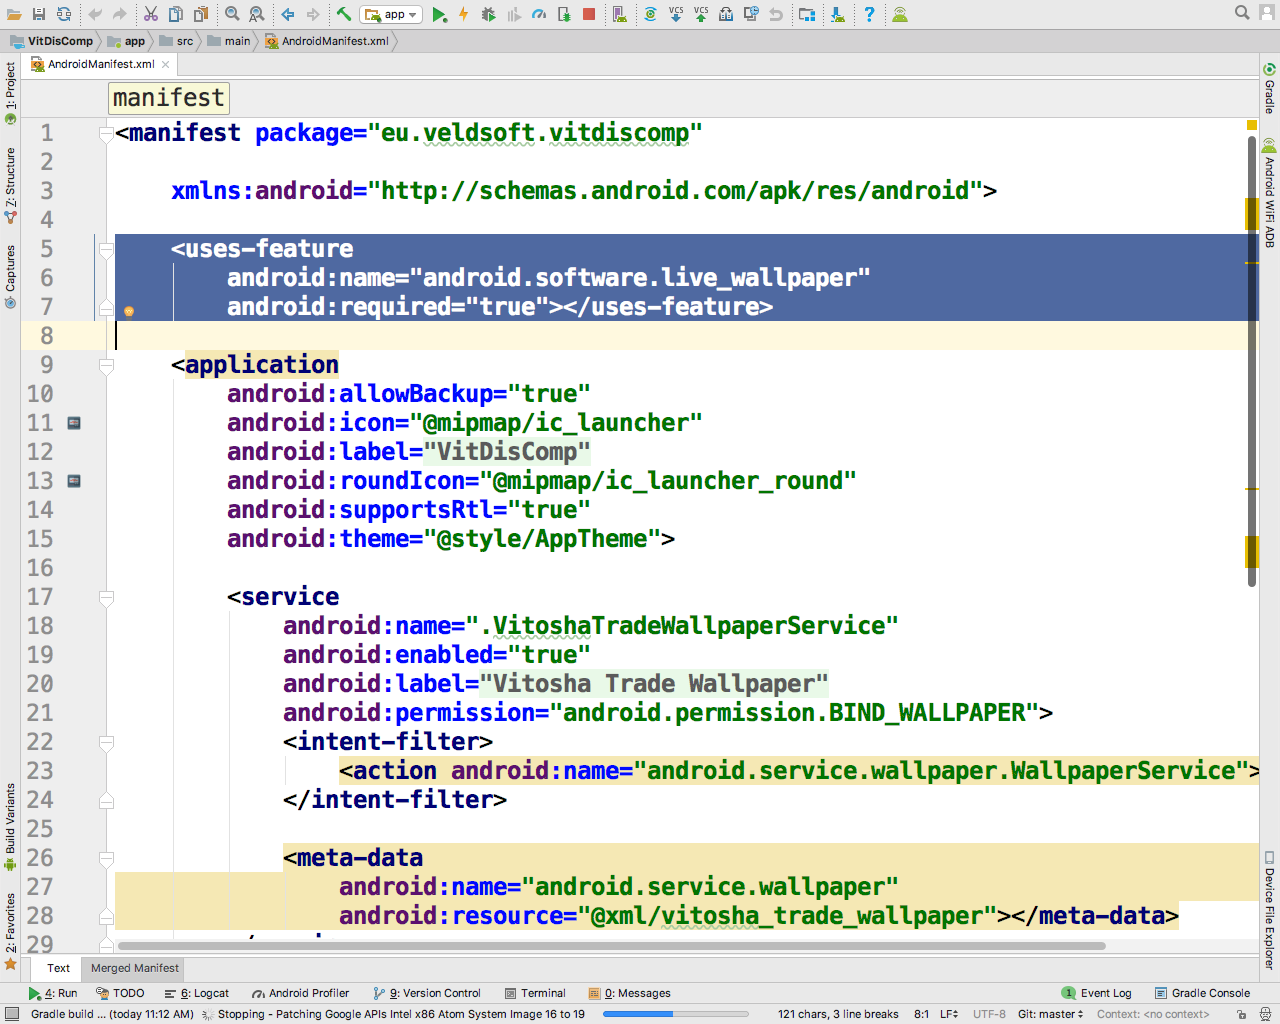
\includegraphics[height=0.45\pdfpageheight]{pic0011}
  \caption{Определяне на приложението като активен тапет.}
\label{fig:pic0011}
\end{figure}
\FloatBarrier

За да се определи приложението като приложение от тип активен тапет е необходимо това изрично да се маркира в манифест файла (Фиг. \ref{fig:pic0011}). Най-съществената полза от тази дефиниция е, че тя предотвратява възможността приложението да бъде инсталирано на устройства, които не поддържат възможностите за визуализация на активен тапет. 

\begin{figure}[h]
  \centering
  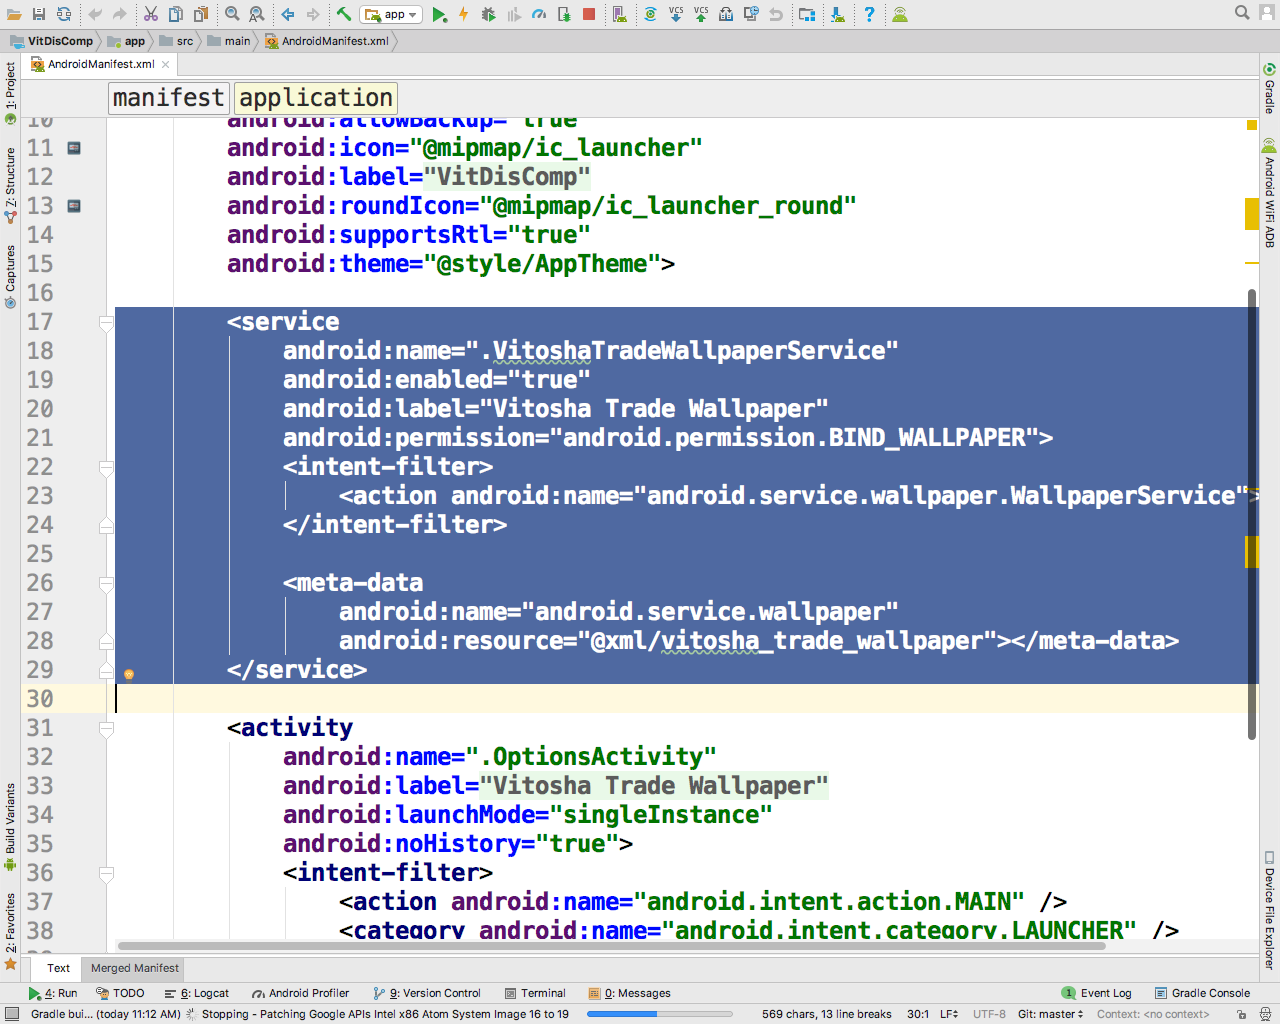
\includegraphics[height=0.45\pdfpageheight]{pic0012}
  \caption{Модул от тип "услуга".}
\label{fig:pic0012}
\end{figure}
\FloatBarrier

Когато в Android се използват много продължителни пресмятания които не са удачни за извършване в нишка е прието тези изчисления да се изнасят в модули без графичен потребителски интерфейс наречени „услуги“ (Service). Работата на активния тапет се извършва точно в такъв модул и поради тази причина в проекта е добавен един (Фиг. \ref{fig:pic0012}).

\begin{figure}[h]
  \centering
  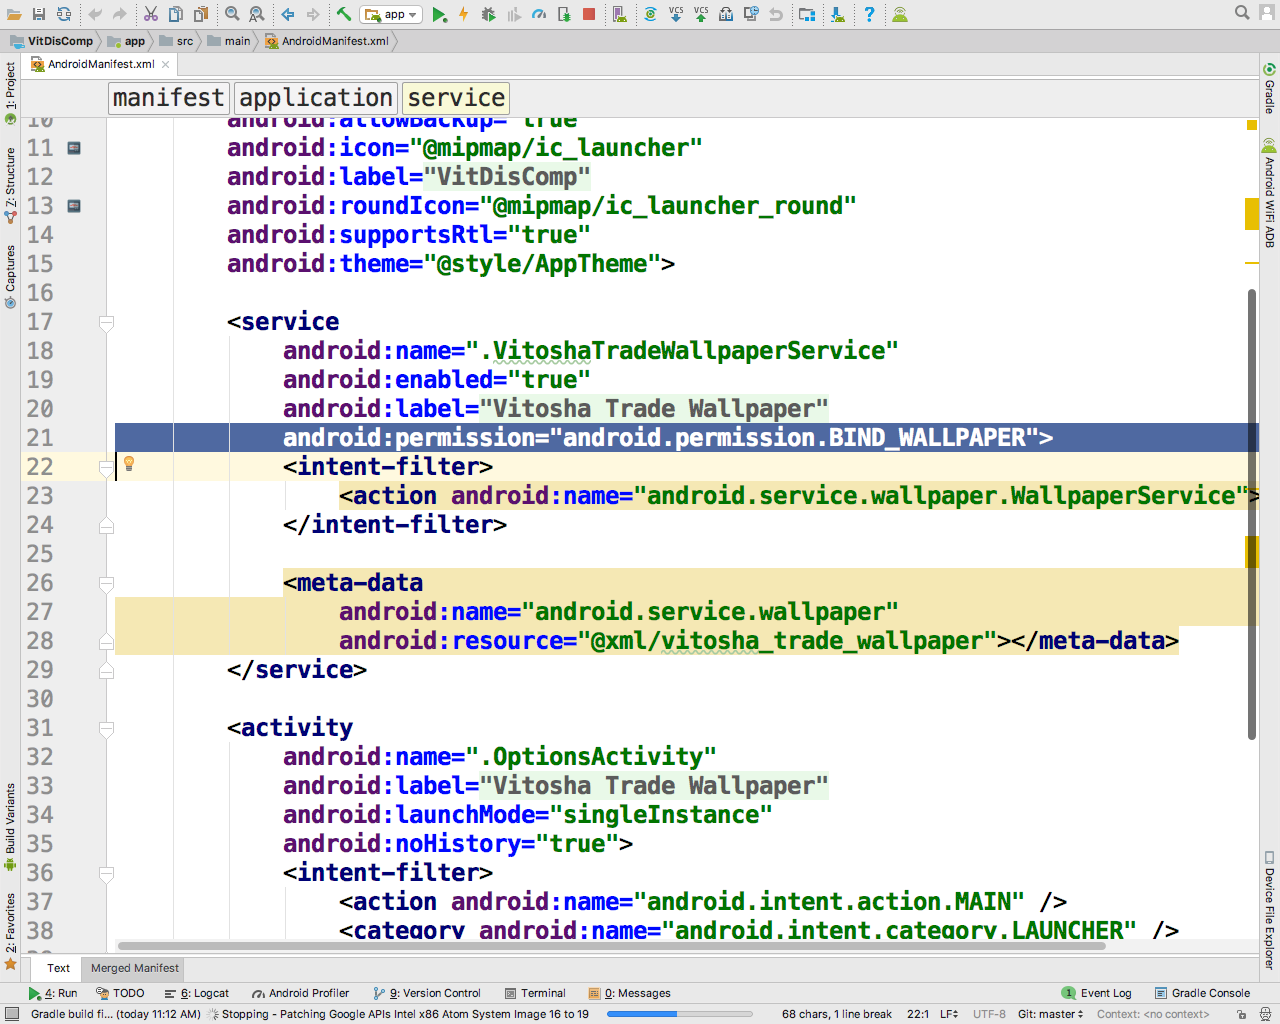
\includegraphics[height=0.45\pdfpageheight]{pic0013}
  \caption{Флагове за достъп до ресурса активен тапет.}
\label{fig:pic0013}
\end{figure}
\FloatBarrier

Моделът за сигурност изисква за всяко по-особено действие да се получи изричното съгласие на потребителя. В случая с активния тапет е необходимо добавянето на android.permission.BIND\_WALLPAPER разрешение (Фиг. \ref{fig:pic0013}).

\begin{figure}[h]
  \centering
  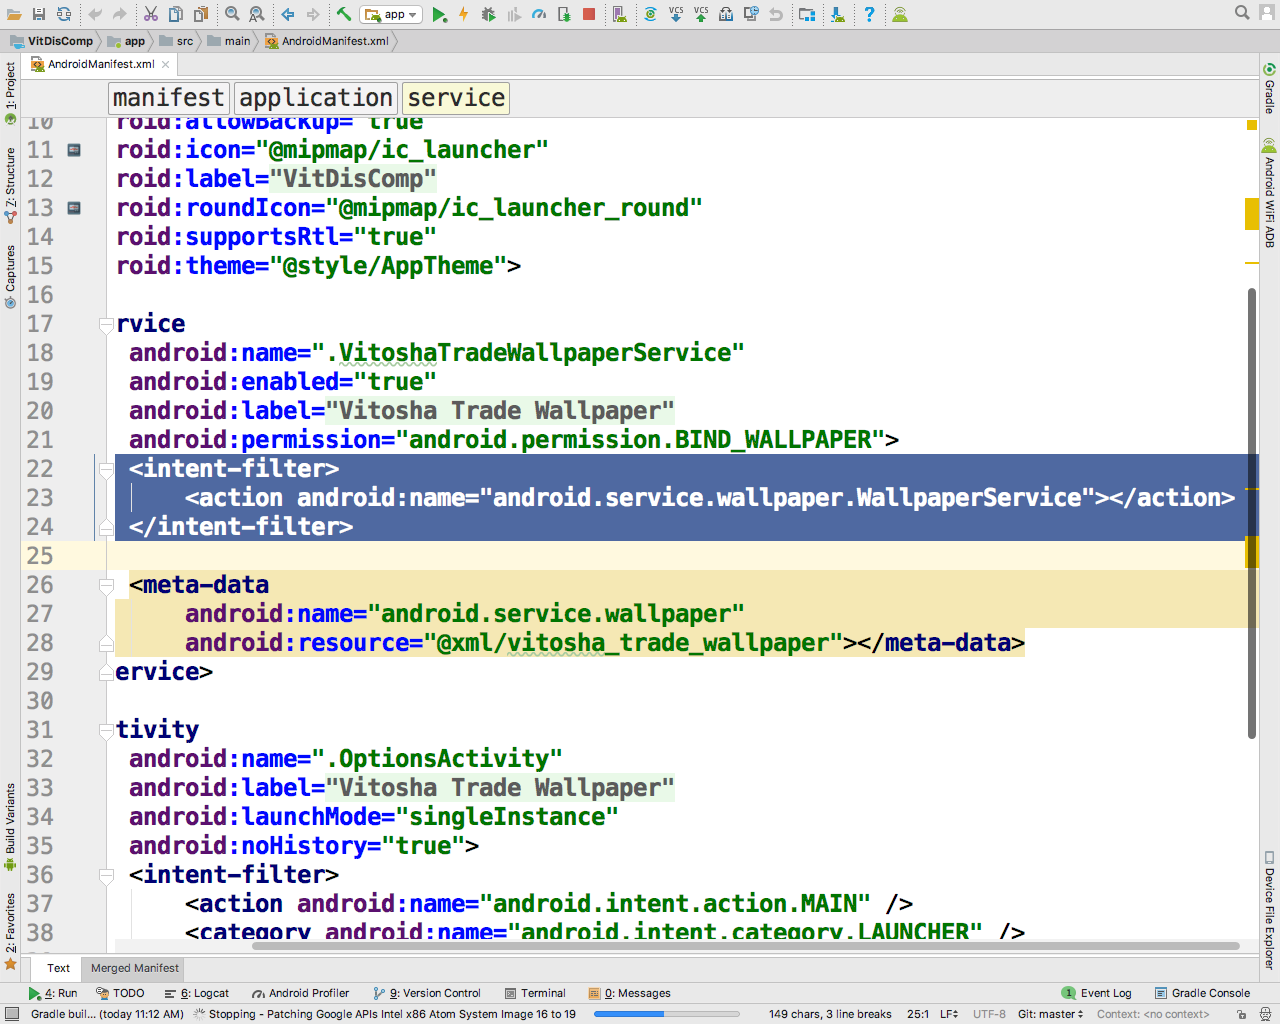
\includegraphics[height=0.45\pdfpageheight]{pic0014}
  \caption{Регистрация на услугата за прослушване на съобщения от операционната система.}
\label{fig:pic0014}
\end{figure}
\FloatBarrier

Освен нуждата от разрешения за ползване на ресурсите за активен тапет е нужно услугата да се абонира за прослушване на съобщения от операционната система (Фиг. \ref{fig:pic0014}).

\begin{figure}[h]
  \centering
  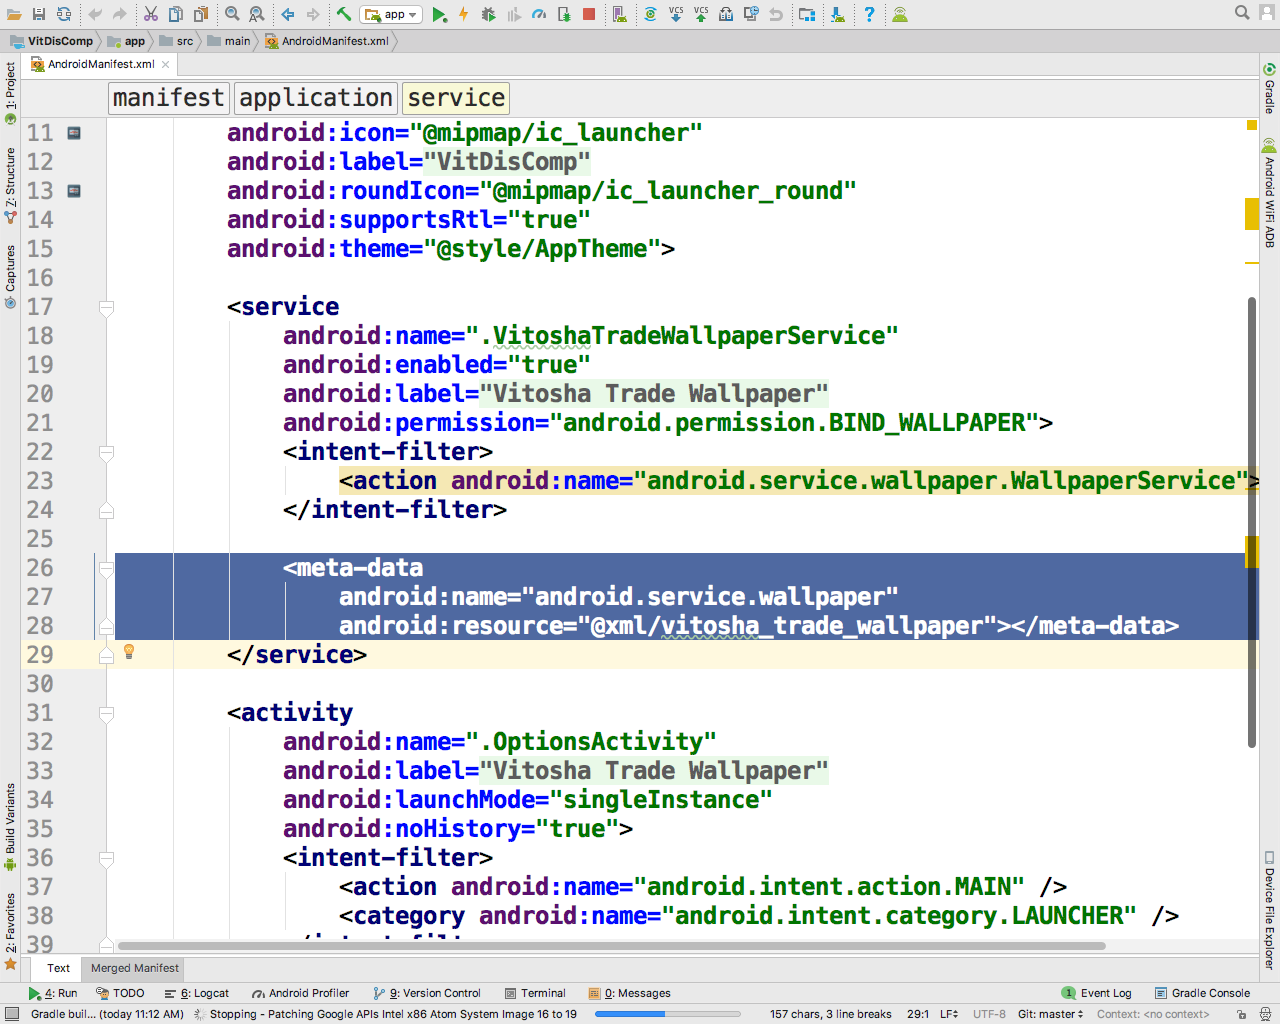
\includegraphics[height=0.45\pdfpageheight]{pic0015}
  \caption{Референция към описателния файл на активния тапет.}
\label{fig:pic0015}
\end{figure}
\FloatBarrier

Описанието на самия активен тапет се съдържа в отделен XML файл, референция към който се посочва в манифеста (Фиг. \ref{fig:pic0015}).

\begin{figure}[h]
  \centering
  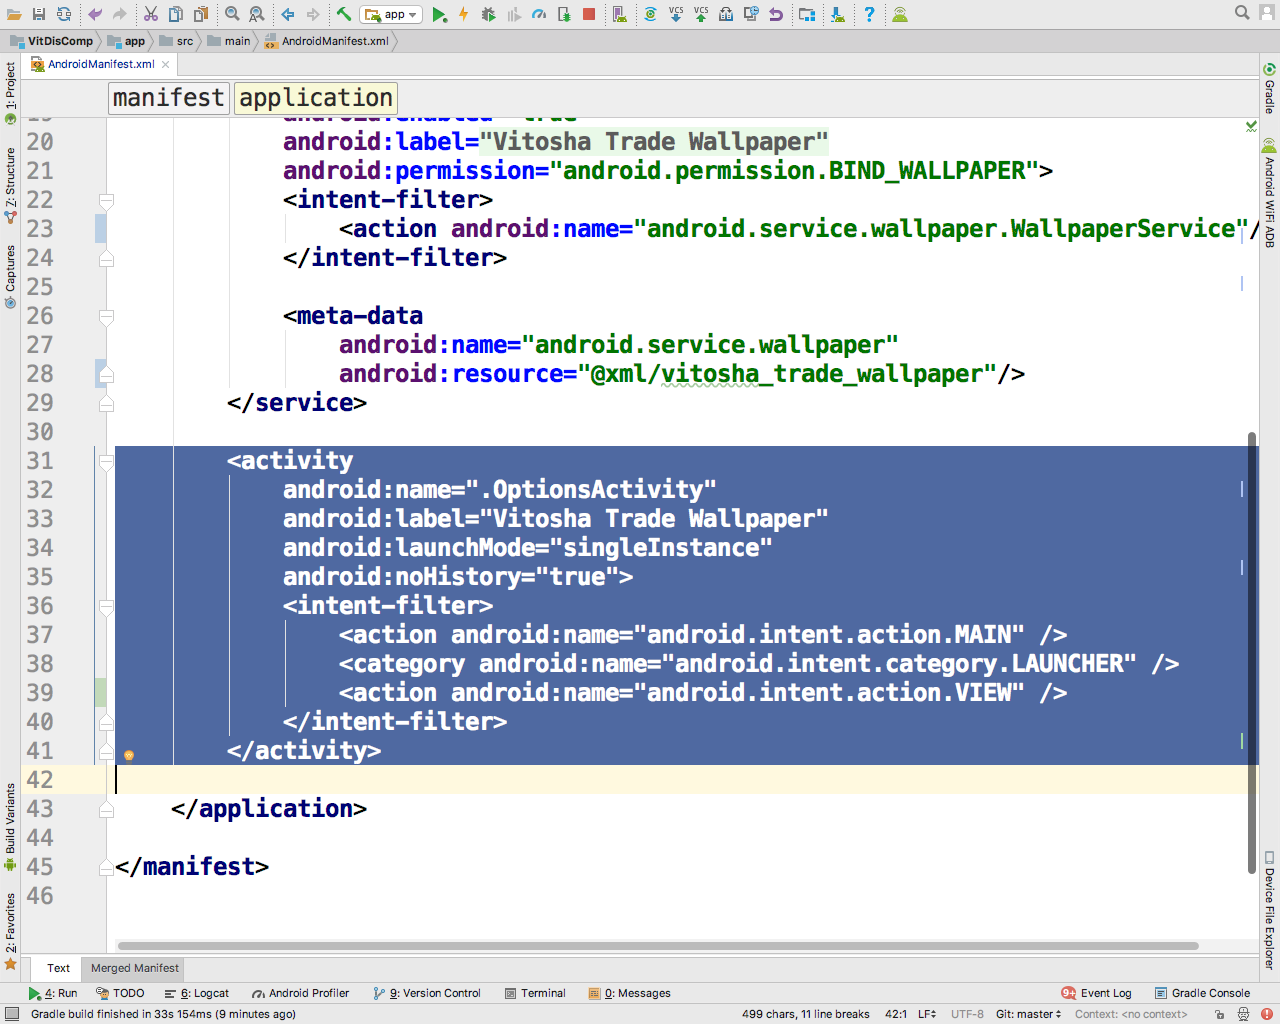
\includegraphics[height=0.45\pdfpageheight]{pic0016}
  \caption{Прозорец за установяване на активния тапет.}
\label{fig:pic0016}
\end{figure}
\FloatBarrier

Последният компонент в такъв тип приложение е прозорец (Android Activity) който да се стартира от операционната система и да служи за установяване на активния тапет (Фиг. \ref{fig:pic0016}). В случая се използва възможността този стартов прозорец да съчетава и функциите на прозорец с опции (Preference Activity).

\begin{figure}[h]
  \centering
  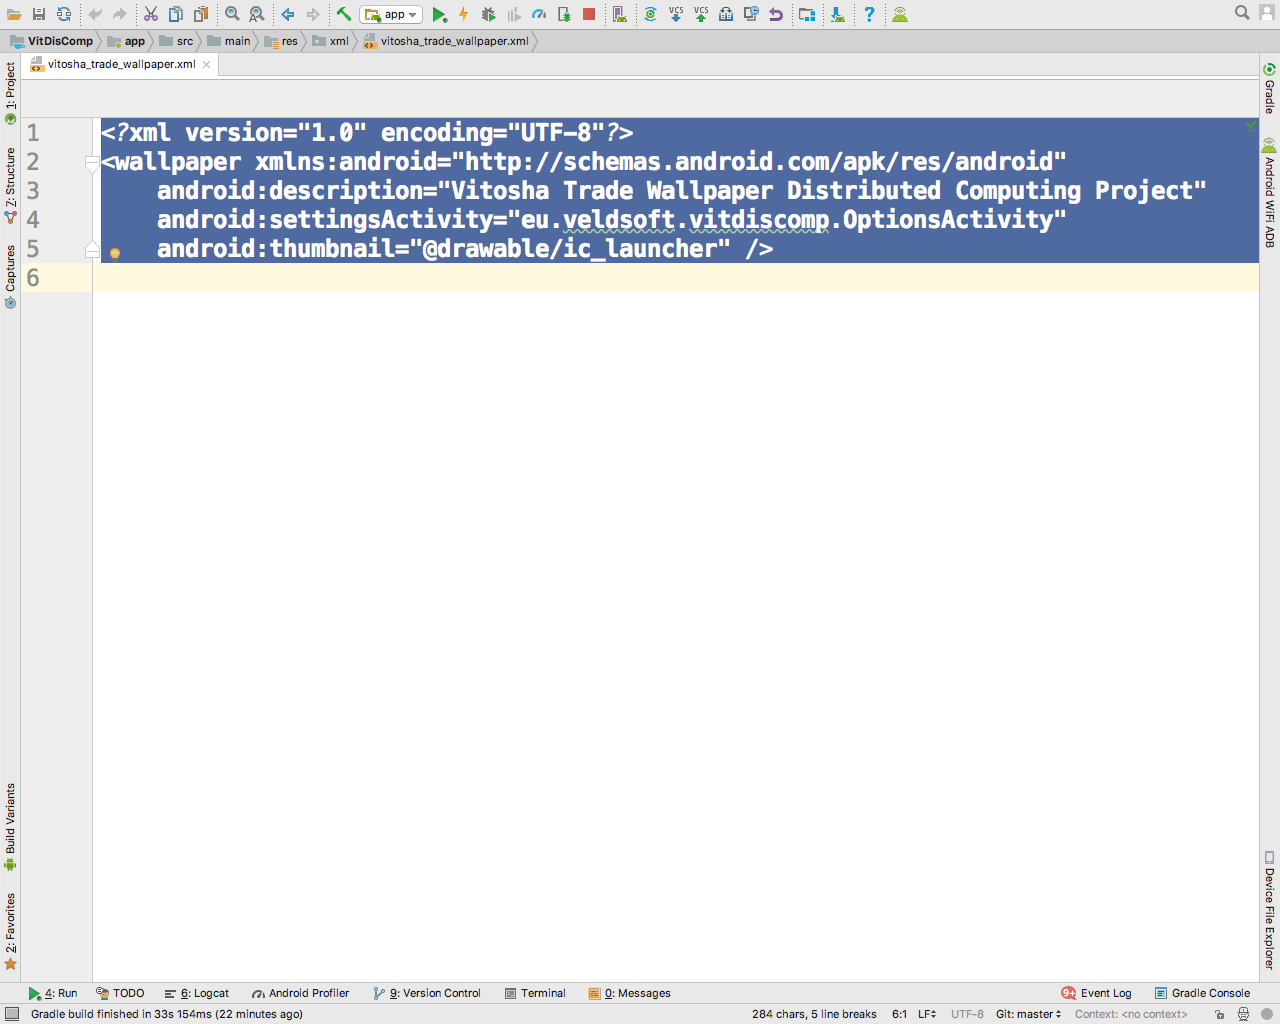
\includegraphics[height=0.45\pdfpageheight]{pic0017}
  \caption{XML описателен файл на тапета.}
\label{fig:pic0017}
\end{figure}
\FloatBarrier

Както вече бе споменато, активният тапет се описва в отделен XML файл, който съдържа кратка анотация на приложението, предварителен изглед, умалена икона и името на прозореца за настройки (Фиг. \ref{fig:pic0017}). 

\section{Екран с настройки}

Тъй като активният тапет ще има и вторична задача да визуализира прогреса на пресмятанията, то е разумно към него да бъде създаден и прозорец с настройки. 

\begin{figure}[h]
  \centering
  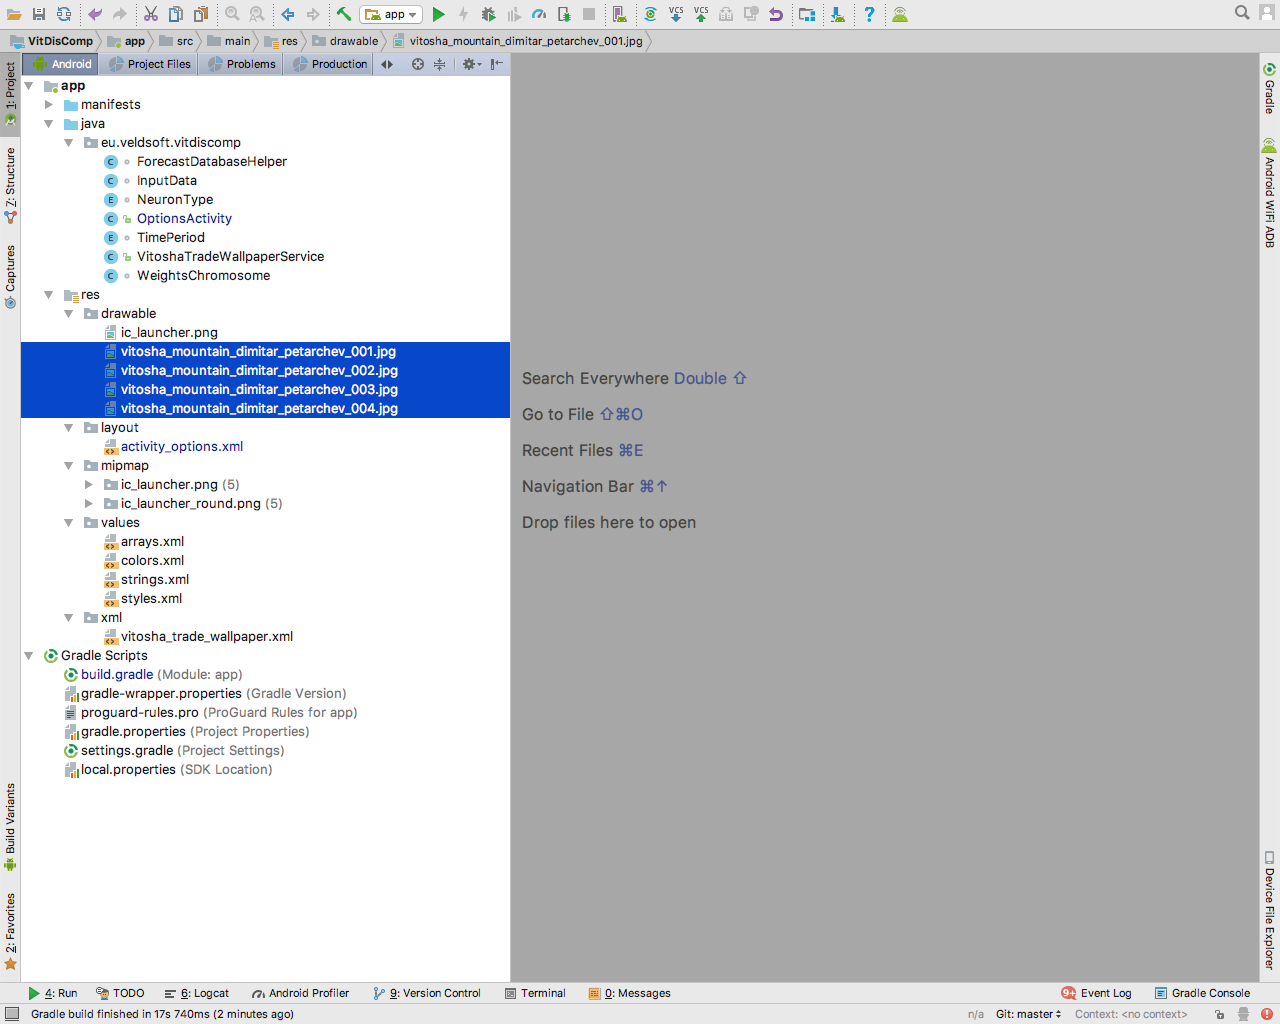
\includegraphics[height=0.45\pdfpageheight]{pic0018}
  \caption{Фотографии на планината Витоша, до град София, България.}
\label{fig:pic0018}
\end{figure}
\FloatBarrier

Като визуализация е избран възможно най-опростен вариант. Няколко фотографии на планината Витоша се визуализират под формата на отрязъци с размерите на екрана който мобилното устройство има (Фиг. \ref{fig:pic0018}). В три полупрозрачни области се визуализира информация за финансовия времеви ред (код и времеви период), стълб-диаграма за входните и изходните данни и текущо състояние на изкуствената невронна мрежа\index{изкуствени невронни мрежи} (Фиг. \ref{fig:pic0019}). 

\begin{figure}[h]
  \centering
  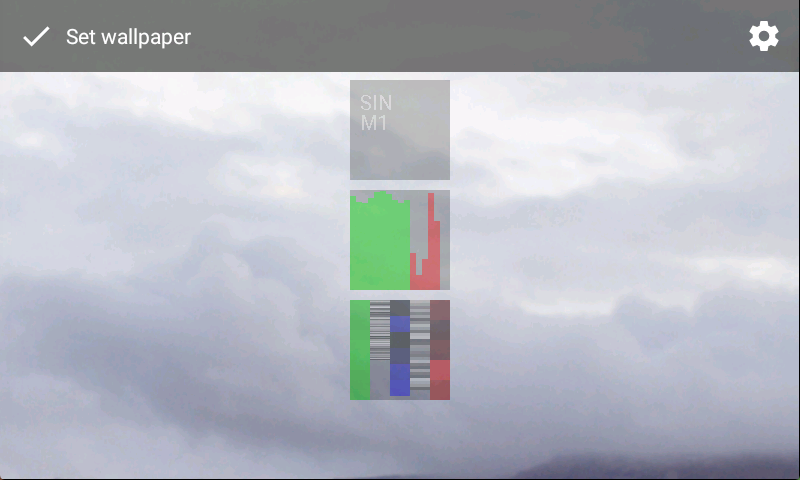
\includegraphics[width=1.0\linewidth]{pic0019}
  \caption{Визуализация на информация от изчисленията.}
\label{fig:pic0019}
\end{figure}
\FloatBarrier

В настройките за активния тапет са предоставени възможности за управление на позицията и размера за трите визуални области. Също така са добавени първоначални настройки за натоварване на устройството и дали активният тапет да бъде включен (Фиг. \ref{fig:pic0020}). 

\begin{figure}[h]
  \centering
  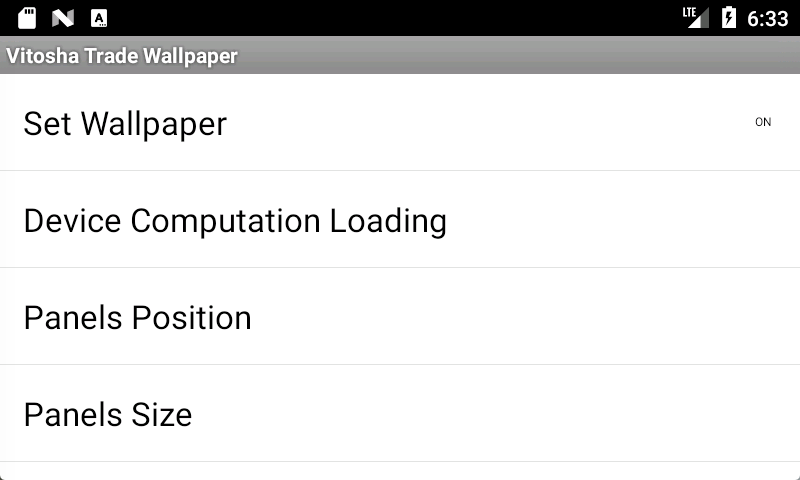
\includegraphics[width=1.0\linewidth]{pic0020}
  \caption{Първоначален набор от настройки.}
\label{fig:pic0020}
\end{figure}
\FloatBarrier

Всеки прозорец в Android се описва със свой файл за разполагане (layout) и файл с Java програмен код. Описателният файл за графичен потребителски интерфейс използва XML и много наподобява съставянето на уеб страница. Когато се изготвя екран за настройки един от най-полезните инструменти в операционната система Android са споделените преференции (Shared Preferences). Те позволяват състоянието на визуалните компоненти директно да бъде запаметено в устройството под формата на ключ-стойност двойки и след това програмно тази информация да бъде използвана. 

\subsection{Описание на потребителския интерфейс под формата на XML файлове}

\begin{figure}[h]
  \centering
  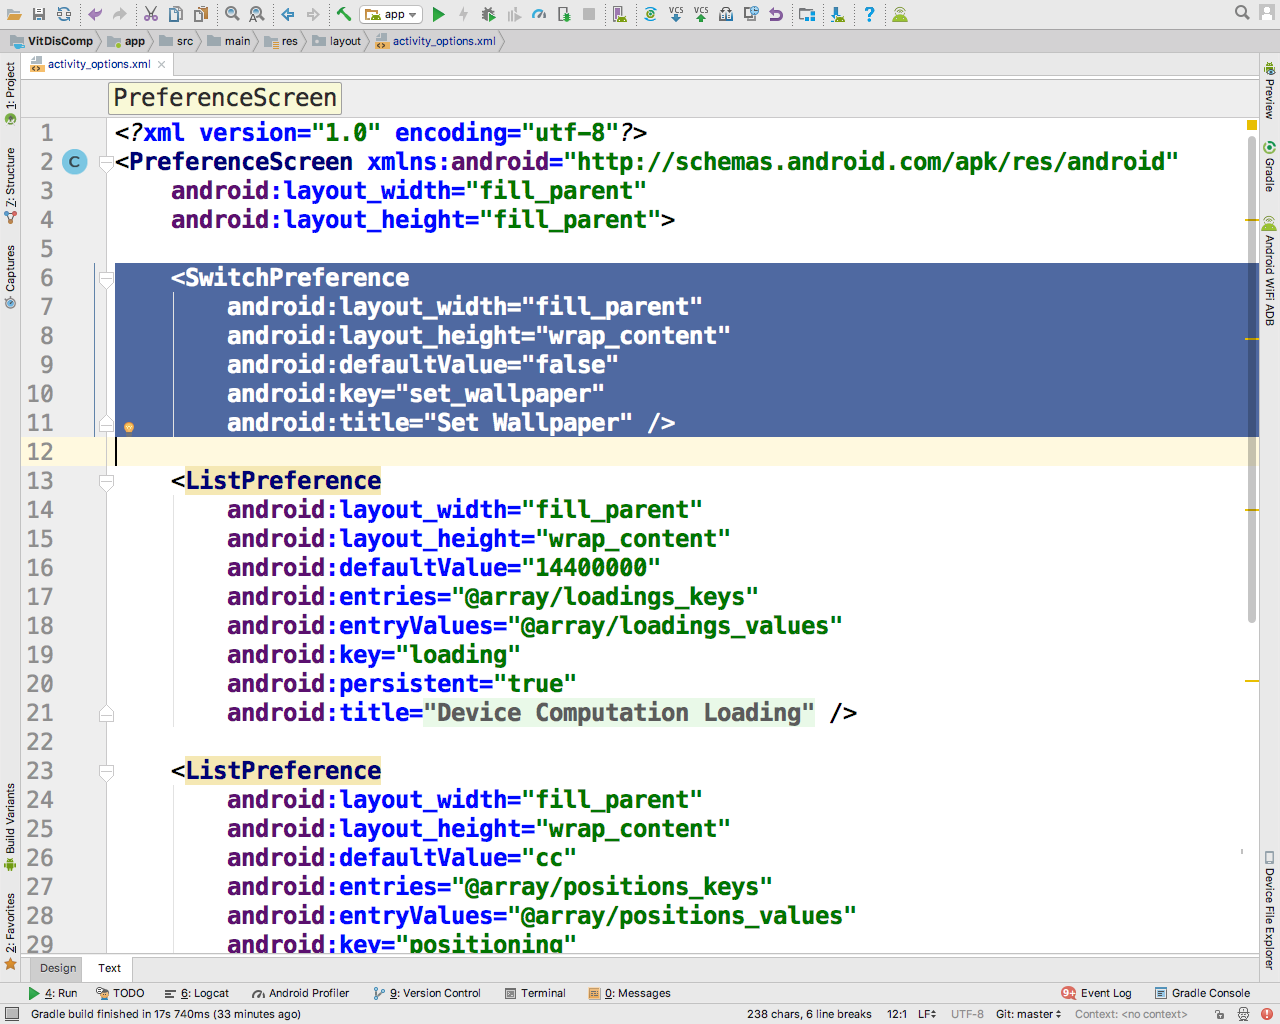
\includegraphics[height=0.45\pdfpageheight]{pic0021}
  \caption{Визуален компонент за включване и изключване на тапета.}
\label{fig:pic0021}
\end{figure}
\FloatBarrier

На първо място е разположен визуален компонент за включване и изключване на активния тапет. Когато ключът е в състояние ON активният тапет бива стартиран, а когато е в позиция OFF активният тапет бива деактивиран (Фиг. \ref{fig:pic0021}). 

\begin{figure}[h]
  \centering
  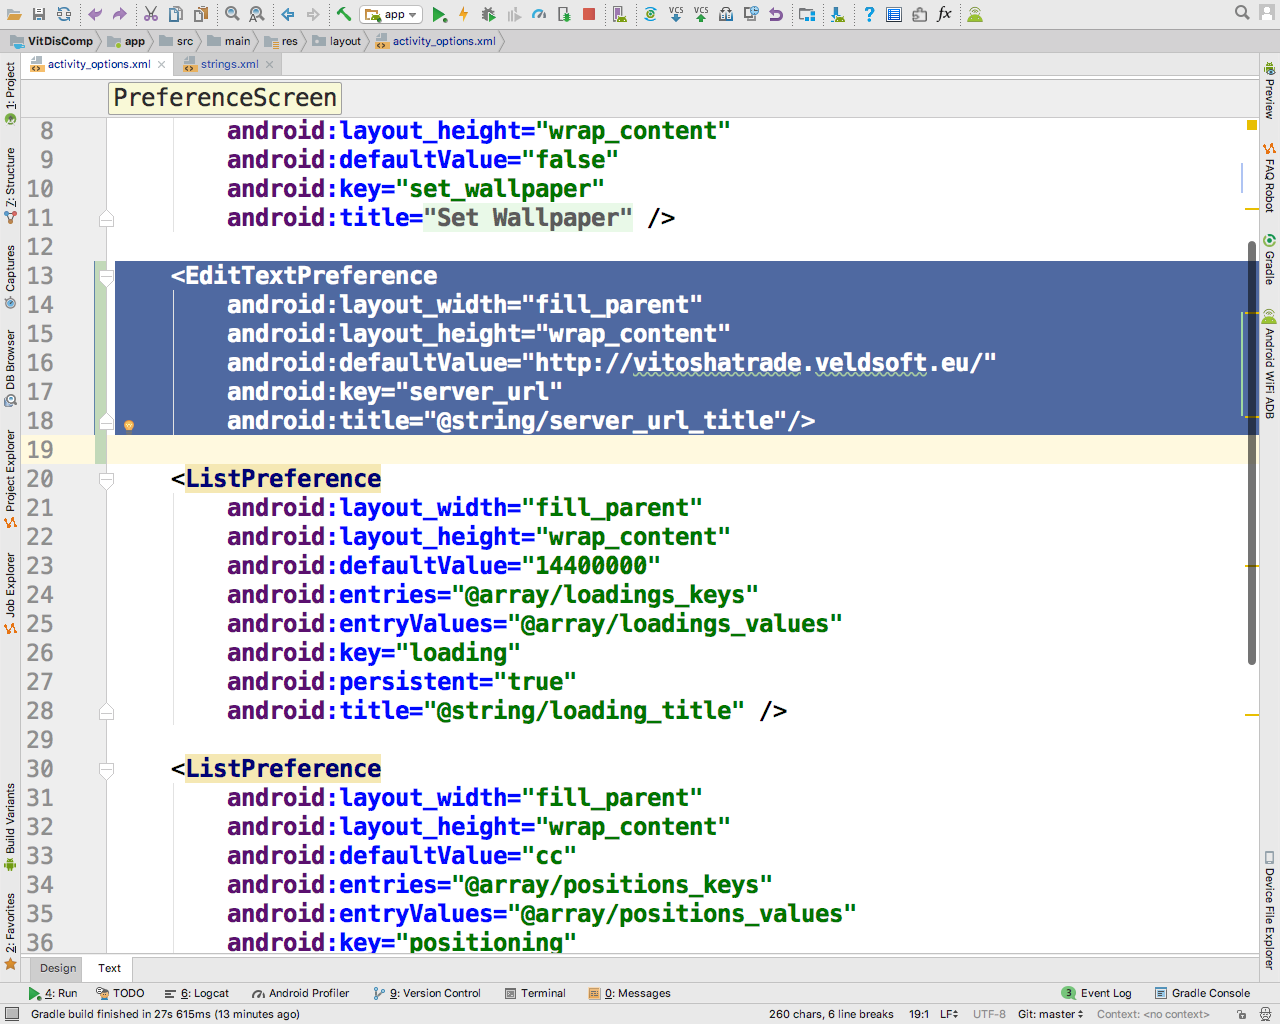
\includegraphics[height=0.45\pdfpageheight]{pic0154}
  \caption{Визуален компонент за посочване на сървър URL.}
\label{fig:pic0154}
\end{figure}
\FloatBarrier

Тъй като мобилното приложение тегли информацията за времевите редове от отдалечен уеб сървър то е подходящо потребителят да има възможност да настройва URL адреса на сървъра с който се работи (Фиг. \ref{fig:pic0154}). Тази опция позволява пренасочване на трафика към други сървъри след като мобилното приложение вече е инсталирано на потребителските мобилни устройства.

\begin{figure}[h]
  \centering
  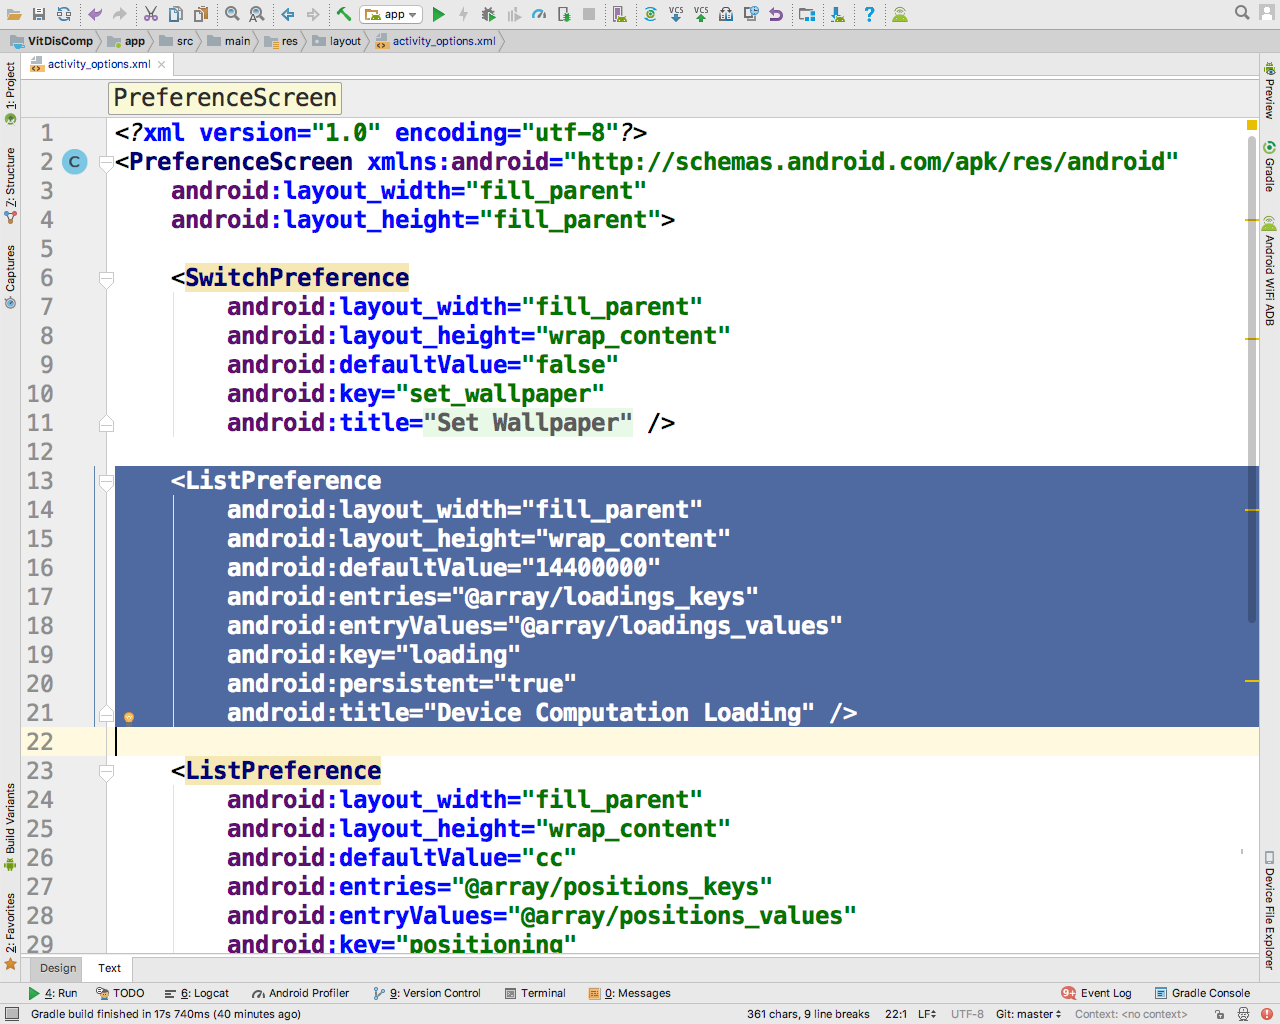
\includegraphics[height=0.45\pdfpageheight]{pic0022}
  \caption{Визуален компонент за регулиране на натоварването.}
\label{fig:pic0022}
\end{figure}
\FloatBarrier

За натоварването на устройството при извършването на фоновите пресмятания се използва списък с предварително дефинирани стойности (Фиг. \ref{fig:pic0022}). 

\begin{figure}[h]
  \centering
  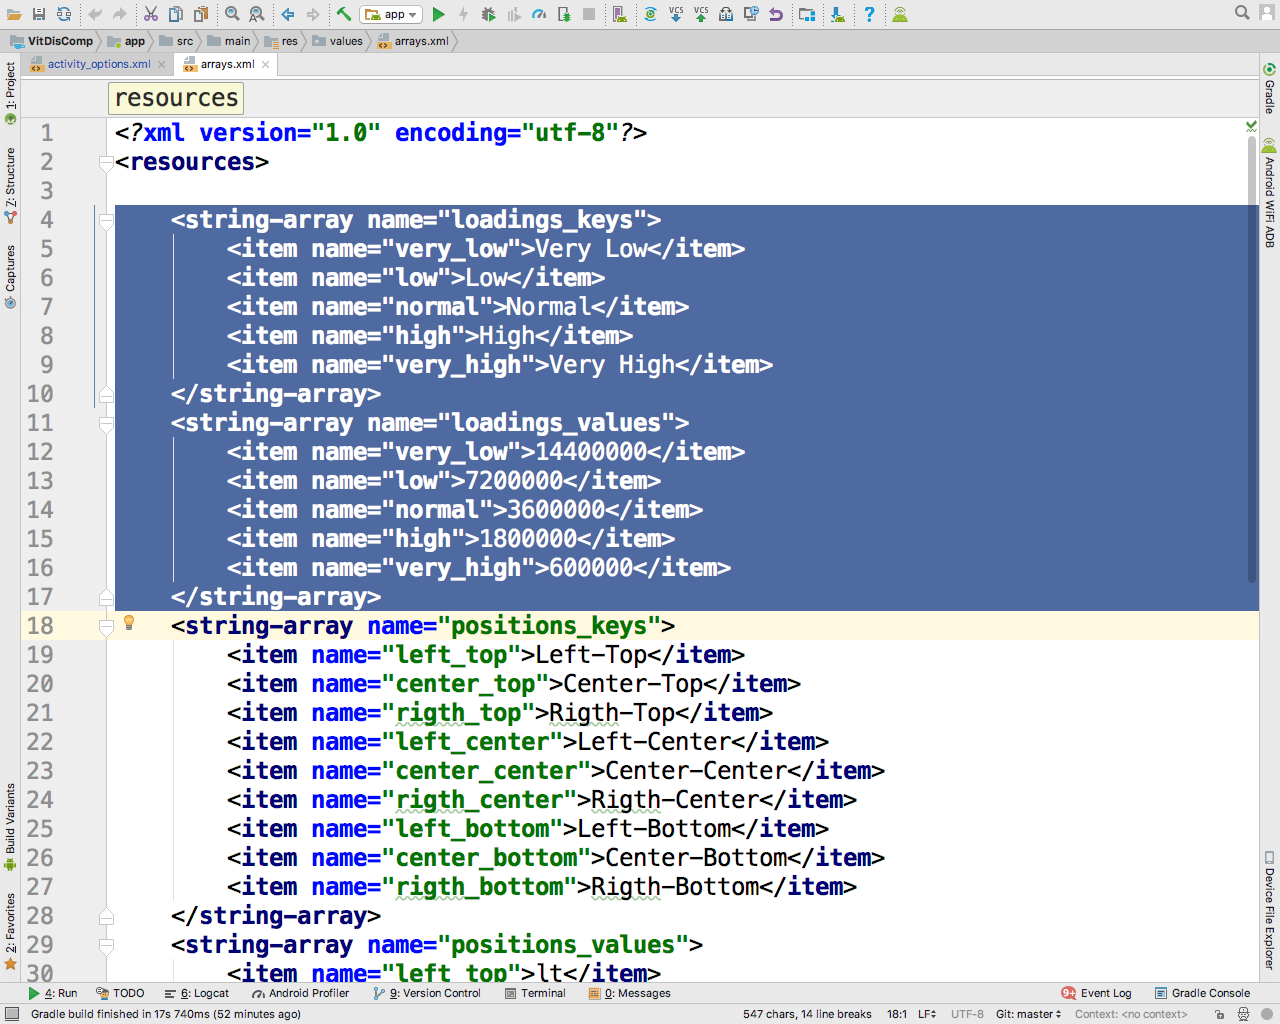
\includegraphics[height=0.45\pdfpageheight]{pic0023}
  \caption{Стойности за натоварване на системата.}
\label{fig:pic0023}
\end{figure}
\FloatBarrier

При проектирането на системата Android една от основните цели е била максимално разделяне на графичния интерфейс от данните. Точно поради тази причина стойностите за натоварване са изнесени в отделен ресурс (Фиг. \ref{fig:pic0023}).

\begin{figure}[h]
  \centering
  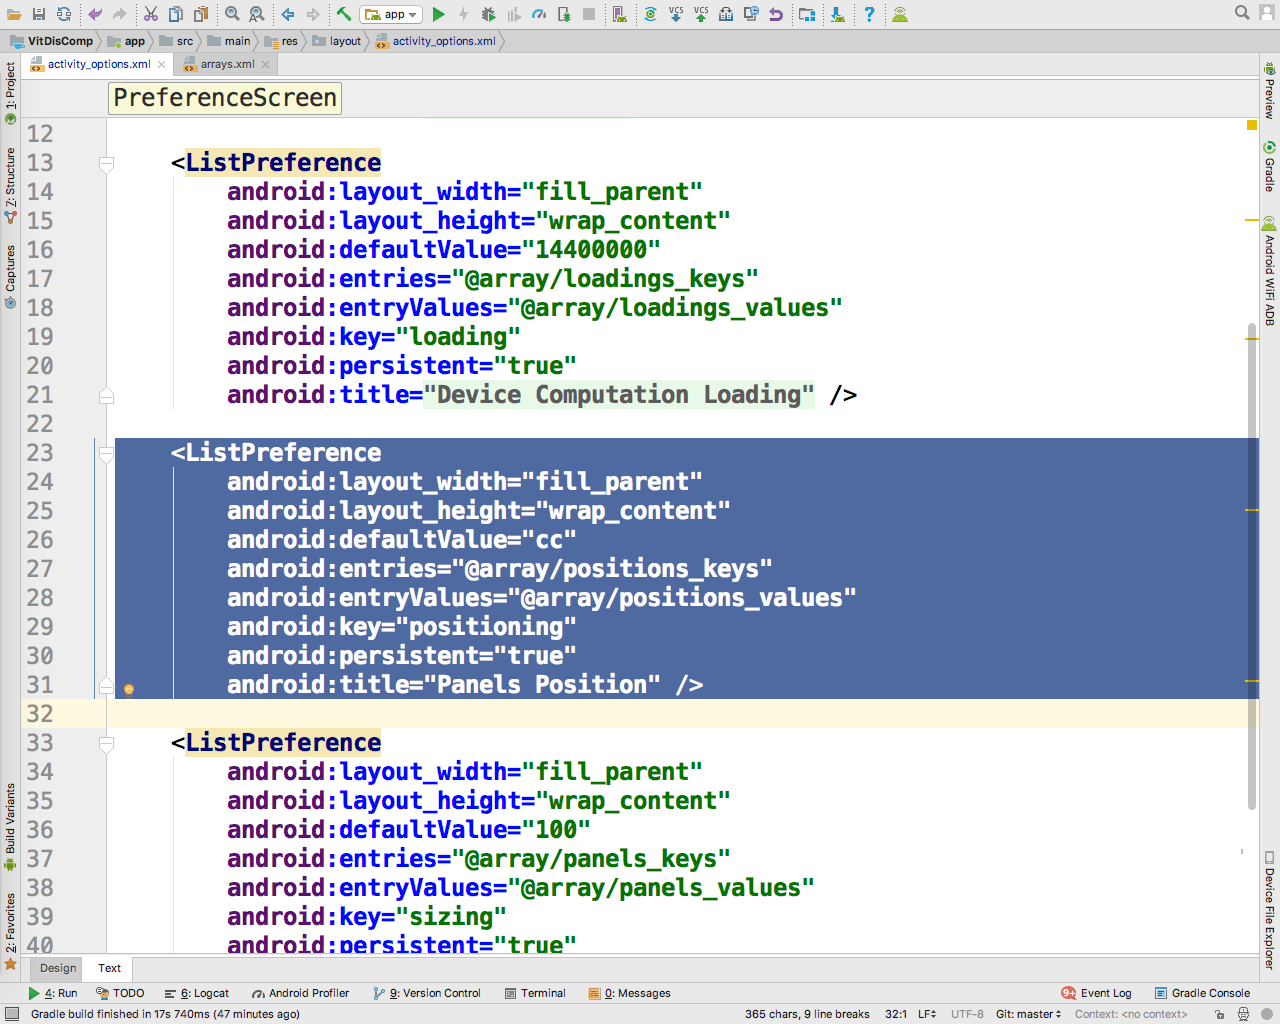
\includegraphics[height=0.45\pdfpageheight]{pic0024}
  \caption{Позициониране на областите за визуализация.}
\label{fig:pic0024}
\end{figure}
\FloatBarrier

Позиционирането на областите за визуализация също се настройва с избор на стойности от списък (Фиг. \ref{fig:pic0024}). 

\begin{figure}[h]
  \centering
  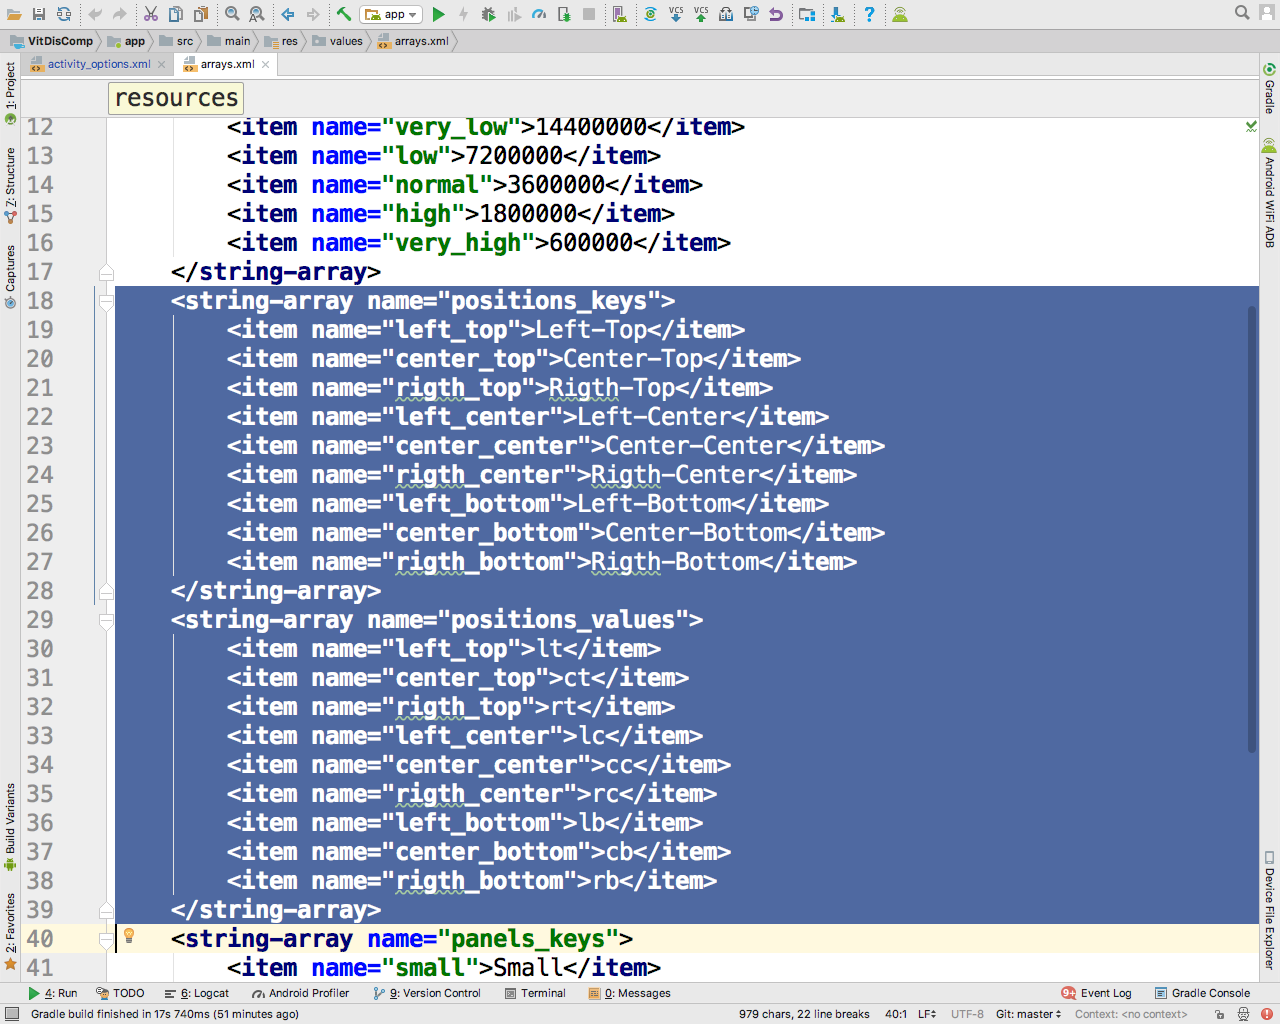
\includegraphics[height=0.45\pdfpageheight]{pic0025}
  \caption{Стойности за позициониране на областите за визуализация.}
\label{fig:pic0025}
\end{figure}
\FloatBarrier

Аналогично на стойностите за натоварване, списъка с възможните позиции на областите за визуализация е изнесен в отделен ресурсен файл (Фиг. \ref{fig:pic0025}). 

\begin{figure}[h]
  \centering
  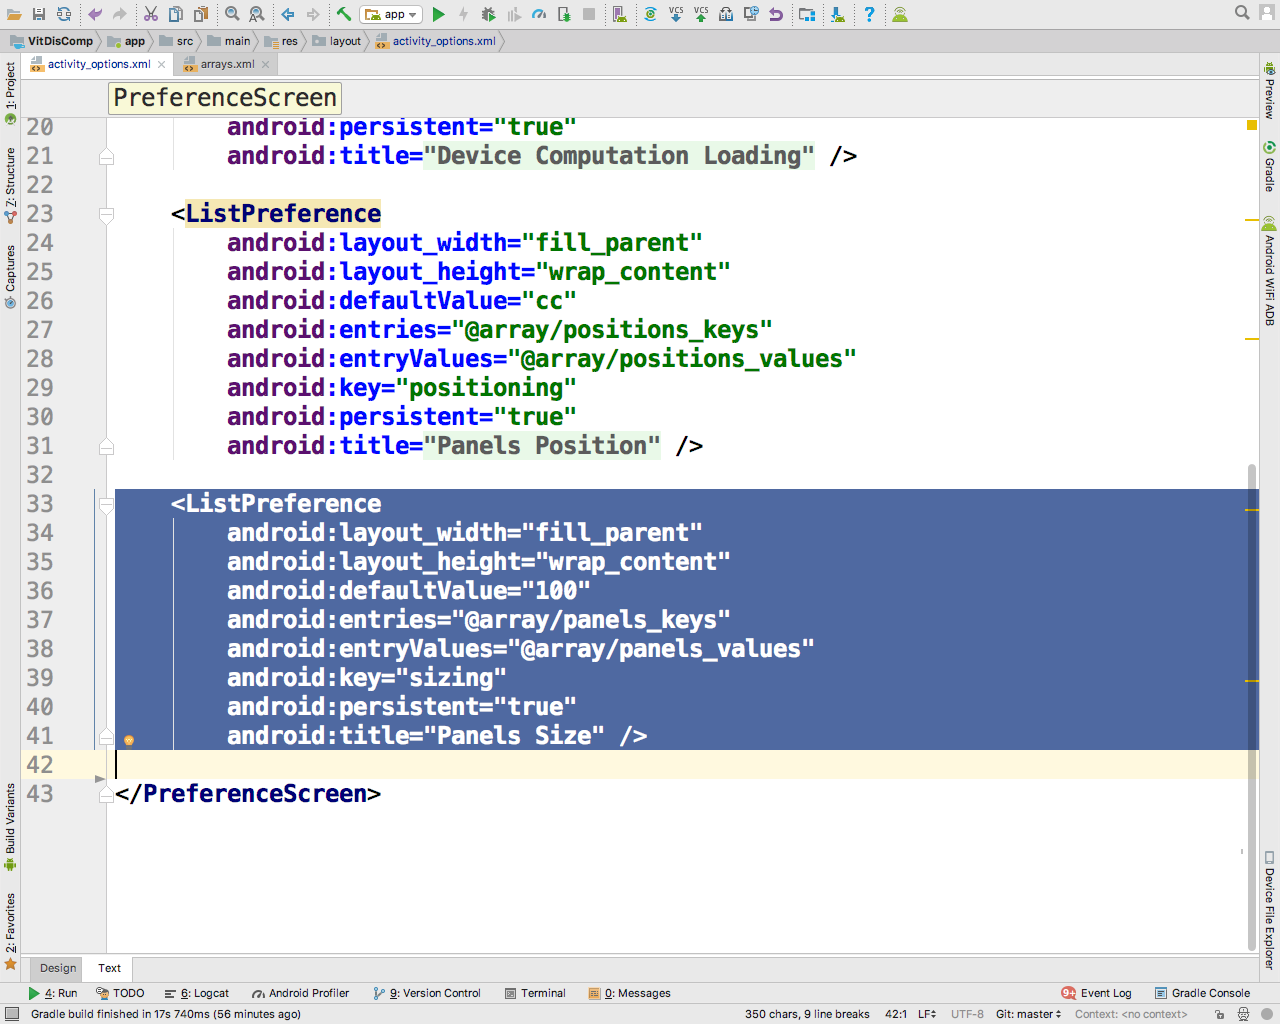
\includegraphics[height=0.45\pdfpageheight]{pic0026}
  \caption{Размер на областите за визуализация.}
\label{fig:pic0026}
\end{figure}
\FloatBarrier

От първоначалните характеристики последна е размерът на областите за визуализация на информацията (Фиг. \ref{fig:pic0026}). 

\begin{figure}[h]
  \centering
  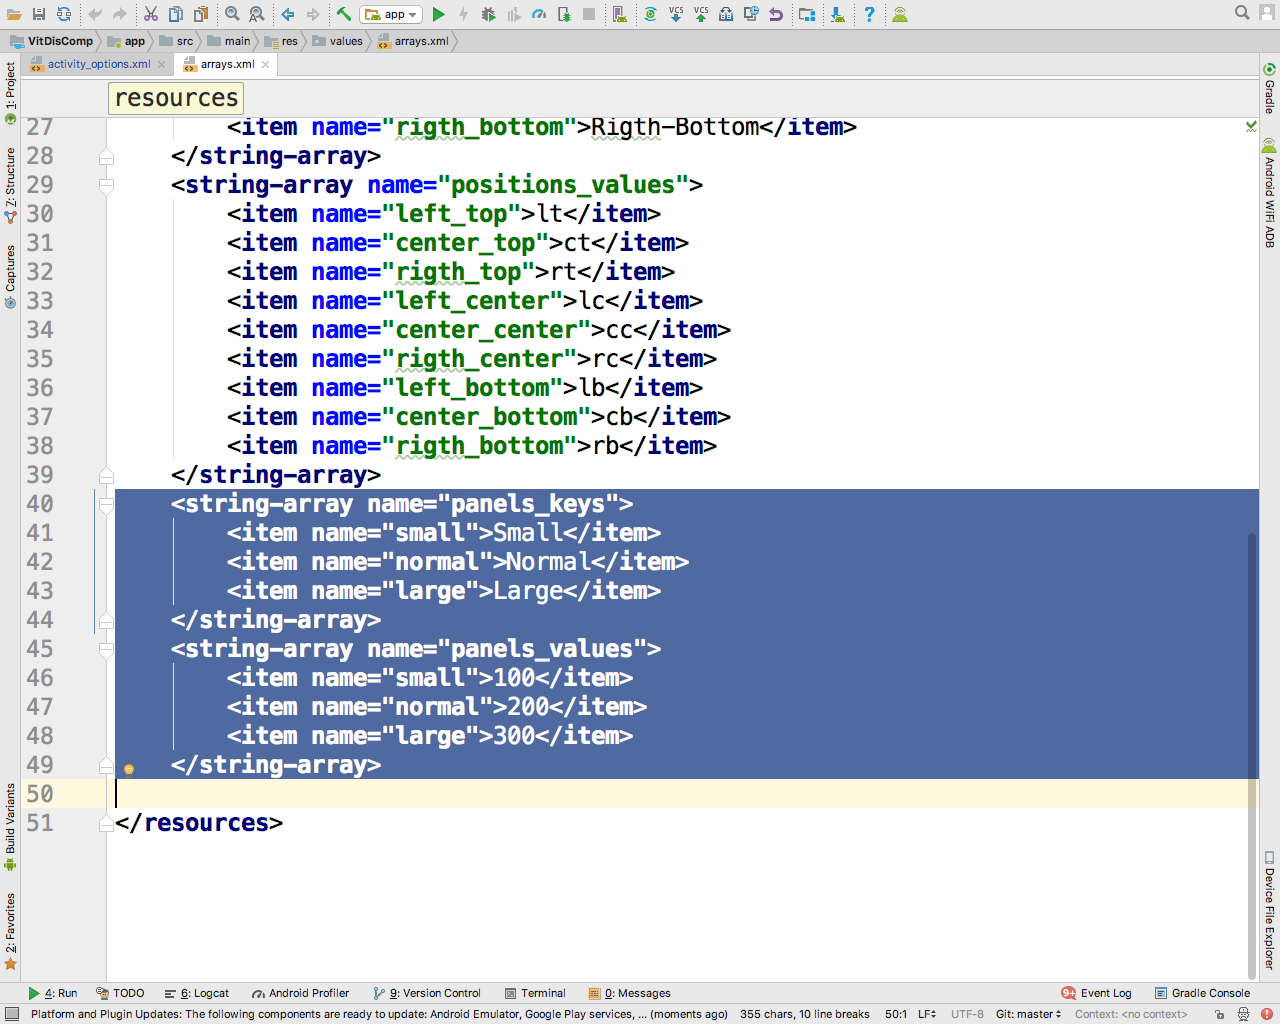
\includegraphics[height=0.45\pdfpageheight]{pic0027}
  \caption{Стойности за размер на областите за визуализация.}
\label{fig:pic0027}
\end{figure}
\FloatBarrier

Областите за визуализация на информацията се предлагат в три размера – малък, среден и голям (Фиг. \ref{fig:pic0027}).

\subsection{Програмен код за управление на интерфейса}

Събитията предизвикани от графичния програмен интерфейс биват прихващани в специално написани за целта Java функции, така че при активирането им да бъдат извършени необходимите програмни действия. За екрана с настройки се прихващат само две събития – създаване и паузиране. 

\begin{figure}[h]
  \centering
  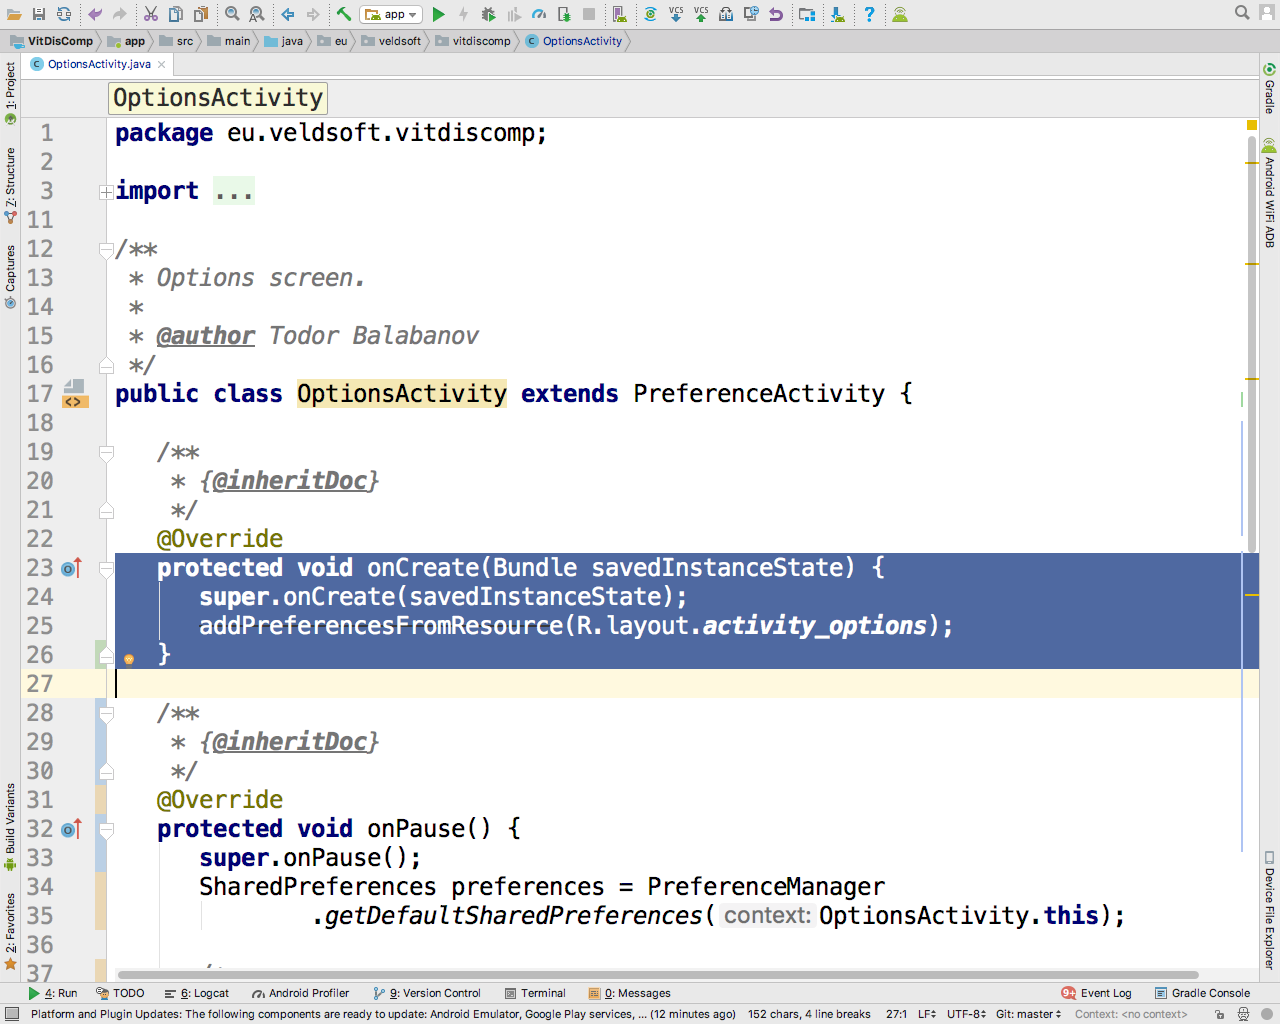
\includegraphics[height=0.45\pdfpageheight]{pic0028}
  \caption{Събитие за създаване на прозореца.}
\label{fig:pic0028}
\end{figure}
\FloatBarrier

Събитието за създаване има за цел да трансформира XML описанието на интерфейса до визуални компоненти, видими за потребителя (Фиг. \ref{fig:pic0028}). 

\begin{figure}[h]
  \centering
  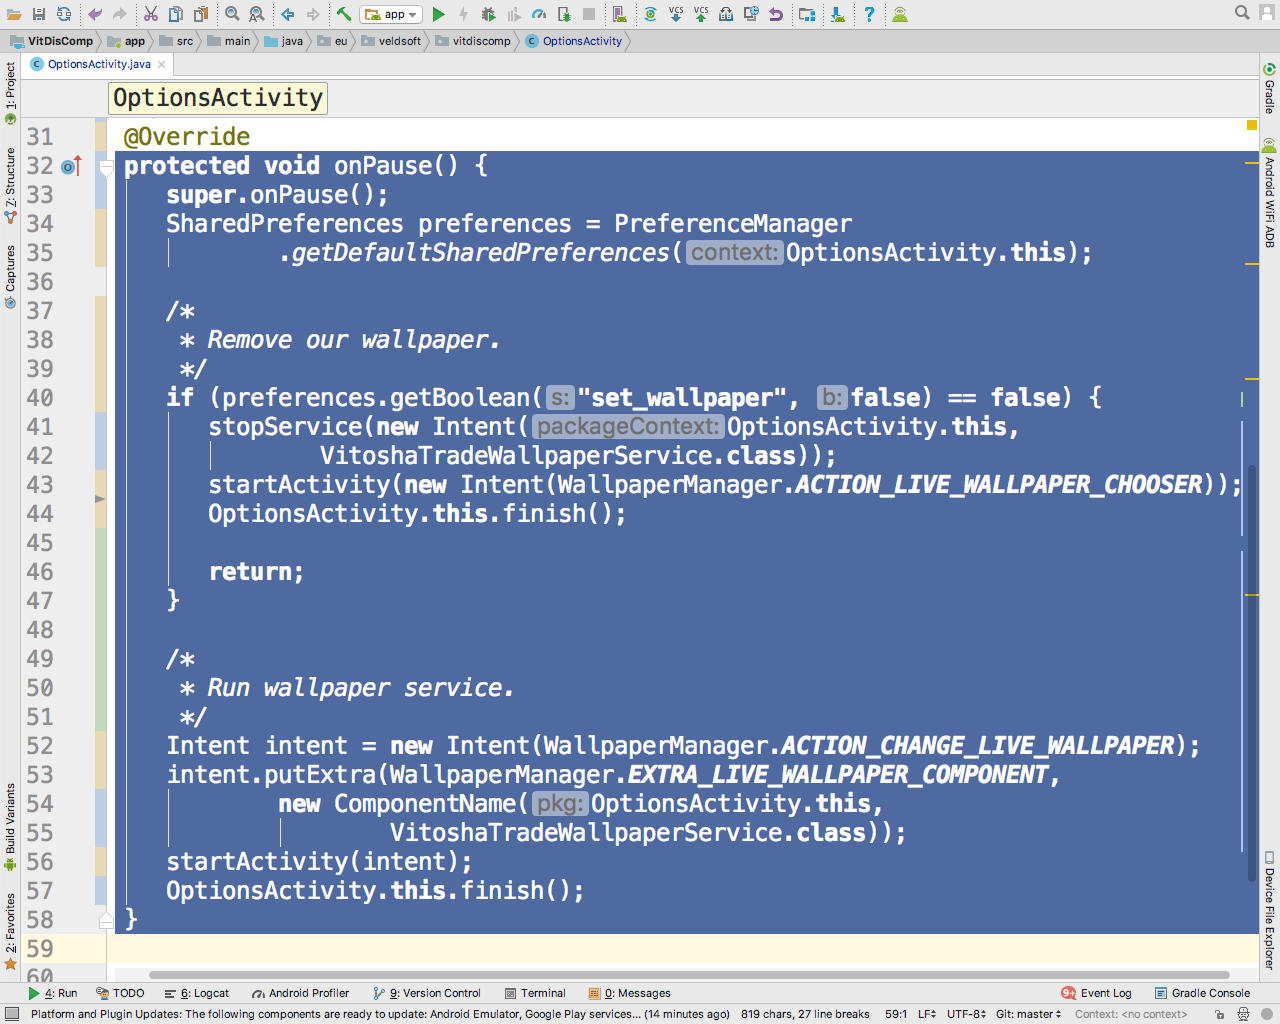
\includegraphics[height=0.45\pdfpageheight]{pic0029}
  \caption{Събитие за пауза на прозореца.}
\label{fig:pic0029}
\end{figure}
\FloatBarrier

При събитието за пауза единствено се взема решение дали активният тапет да бъде стартиран или да бъде спрян (Фиг. \ref{fig:pic0029}). 

\section{Пресмятане на фонов режим}

Продължителните пресмятания, които не изискват графичен потребителски интерфейс се осъществяват в модули наречени „услуги“ (Service). Когато става въпрос за активен тапет е необходимо да се напише собствен клас който е наследник на класа WallpaperService (Фиг. \ref{fig:pic0030}).

\begin{figure}[h]
  \centering
  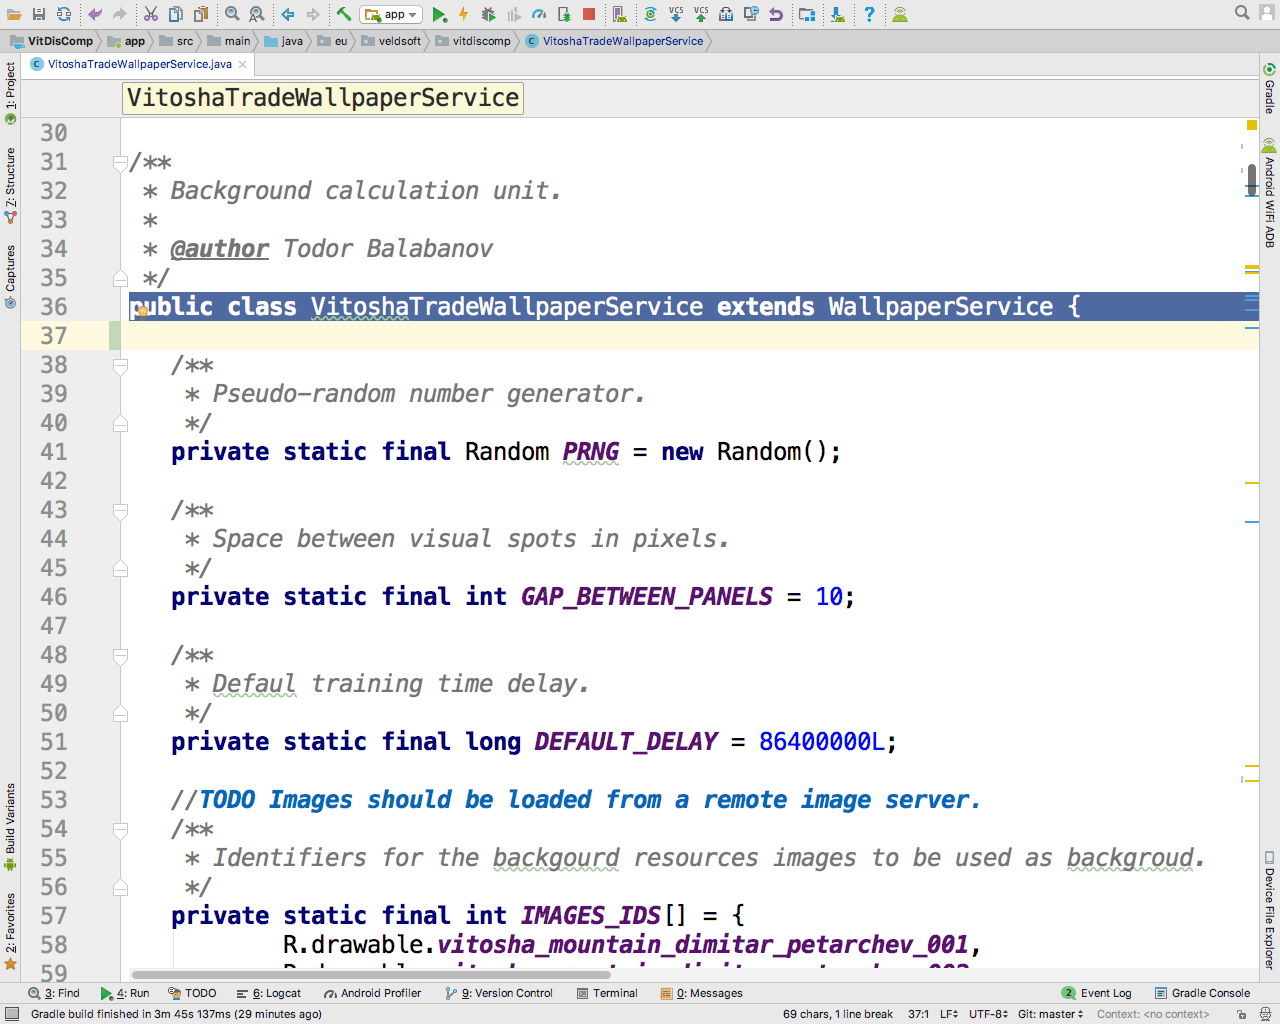
\includegraphics[height=0.45\pdfpageheight]{pic0030}
  \caption{Наследяване на WallpaperService.}
\label{fig:pic0030}
\end{figure}
\FloatBarrier

Група от константи спомагат за генерирането на случайни числа, определяне на разстояние между зоните за визуализация и подразбираща се стойност за времето между две отделни стартирания на тренировъчния алгоритъм (Фиг. \ref{fig:pic0031}). 

\begin{figure}[h]
  \centering
  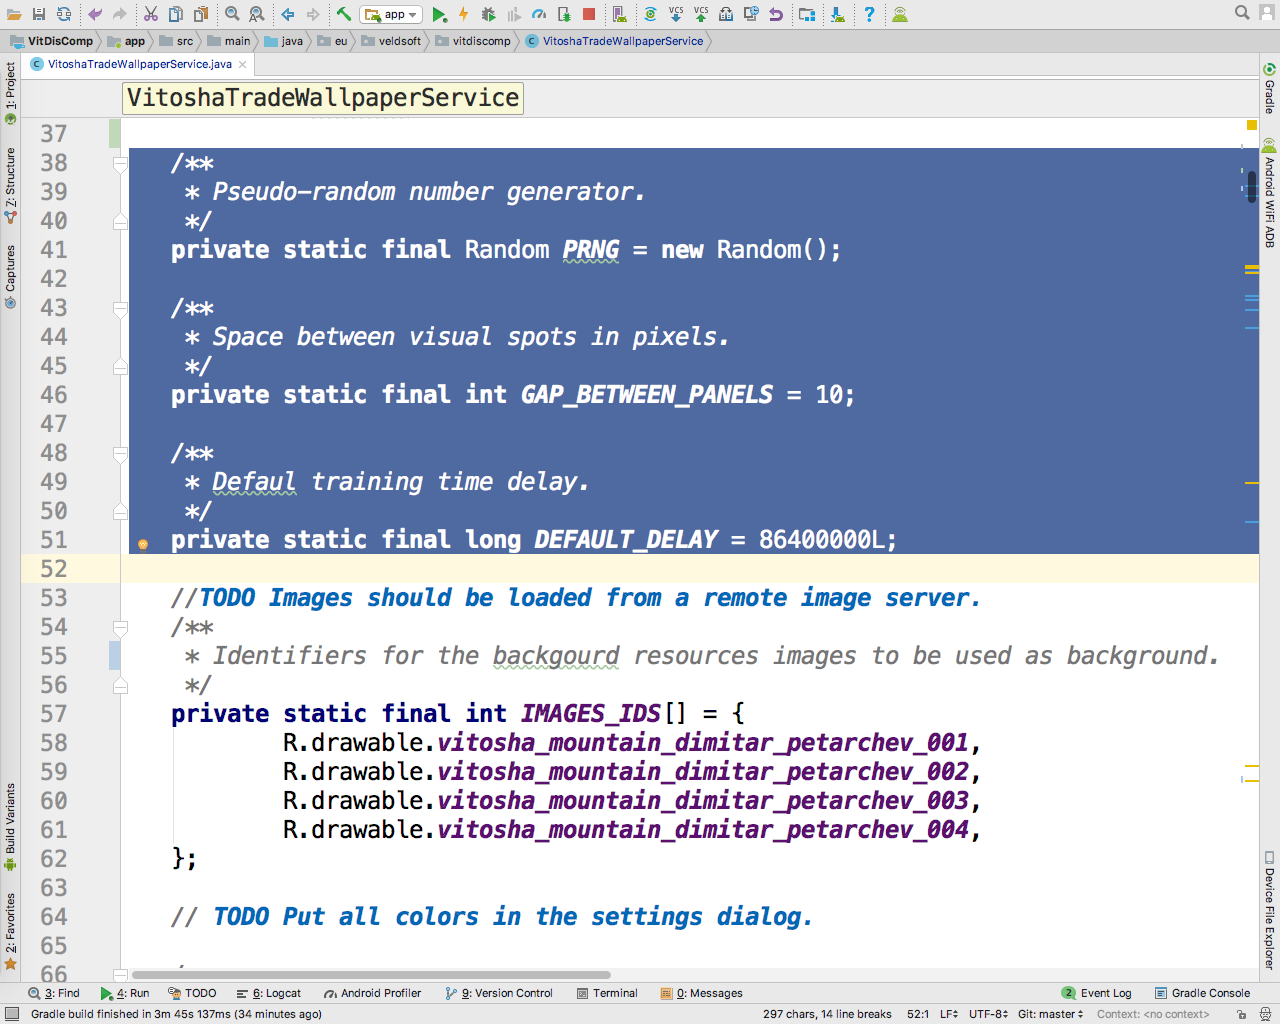
\includegraphics[height=0.45\pdfpageheight]{pic0031}
  \caption{Спомагателни константи.}
\label{fig:pic0031}
\end{figure}
\FloatBarrier

Цветовете използвани за визуализацията също са зададени с група от константи, но в последствие ще бъдат превърнати в настройки със стойности от прозореца за настройки (Фиг. \ref{fig:pic0032}).

\begin{figure}[h]
  \centering
  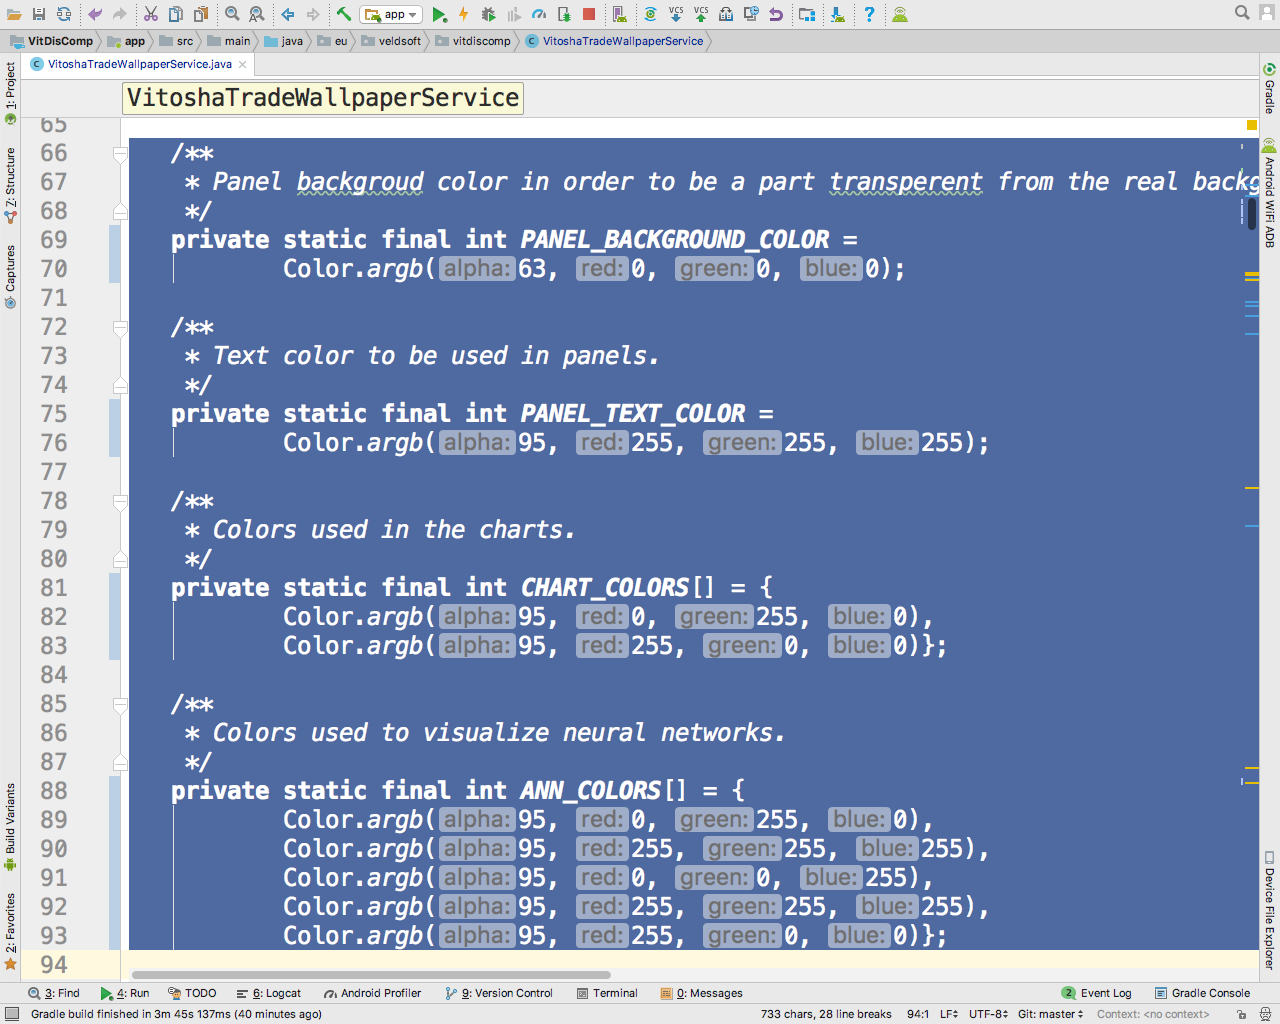
\includegraphics[height=0.45\pdfpageheight]{pic0032}
  \caption{Константи за цветовете.}
\label{fig:pic0032}
\end{figure}
\FloatBarrier

Група променливи отговарят за състоянието на активния тапет. Това включва – размери на екрана, време между отделните обучения на изкуствената невронна мрежа, дали активният тапет е включен или изключен и точната позиция на зоните за визуализация на информацията от процеса по обучение на изкуствената невронна мрежа (Фиг. \ref{fig:pic0033}). 

\begin{figure}[h]
  \centering
  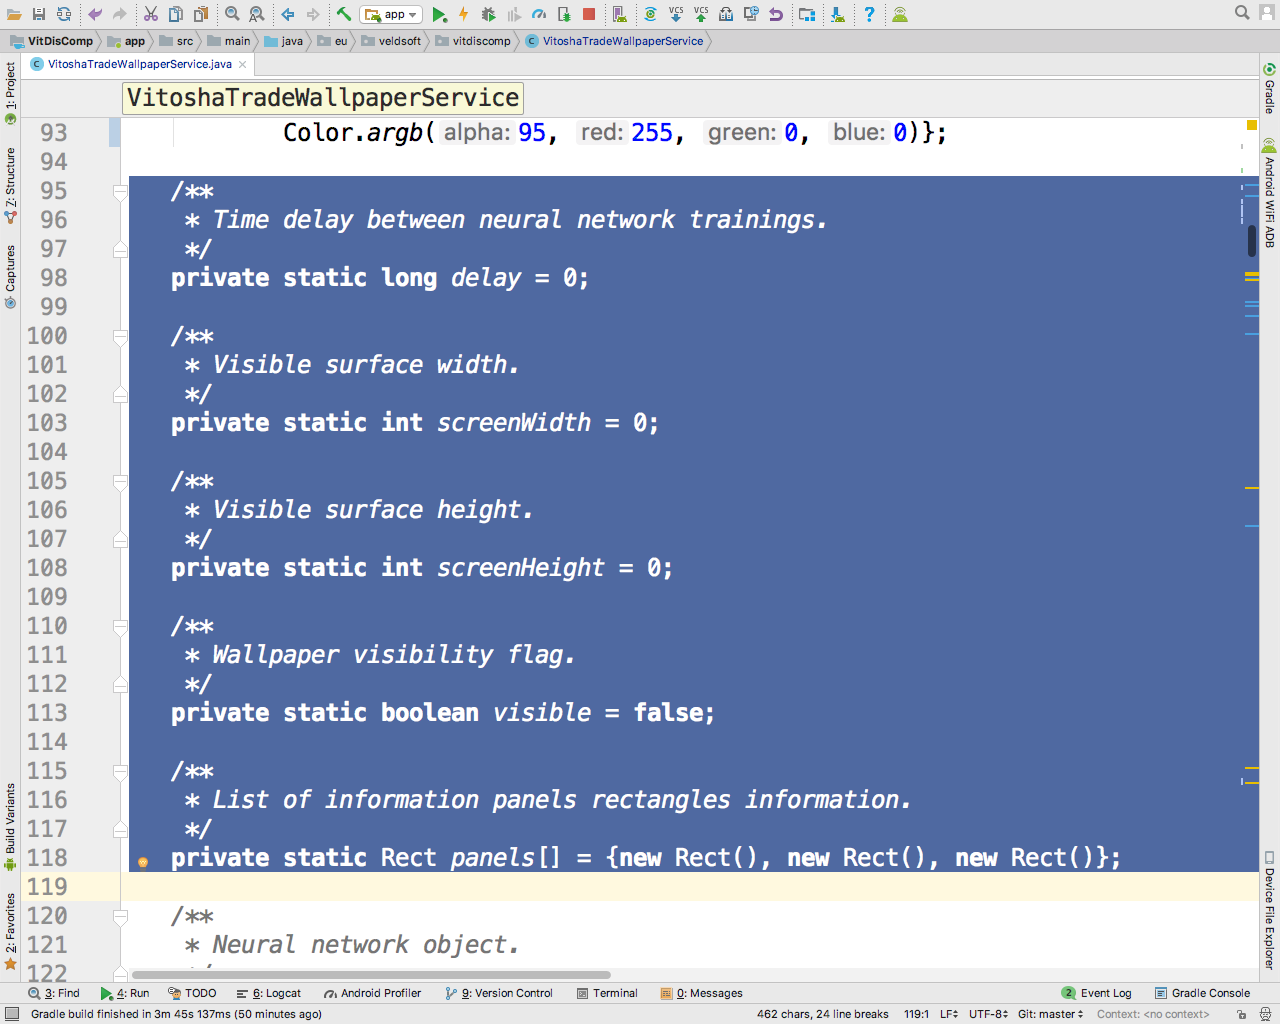
\includegraphics[height=0.45\pdfpageheight]{pic0033}
  \caption{Променливи отразяващи състоянието на активния тапет.}
\label{fig:pic0033}
\end{figure}
\FloatBarrier

Друга група променливи (референции към обекти) поемат отговорността за управлението на изкуствената невронна мрежа, тренировъчните примери, входно-изходните данни към мрежата и правилото за нейното обучение (Фиг. \ref{fig:pic0034}).

\begin{figure}[h]
  \centering
  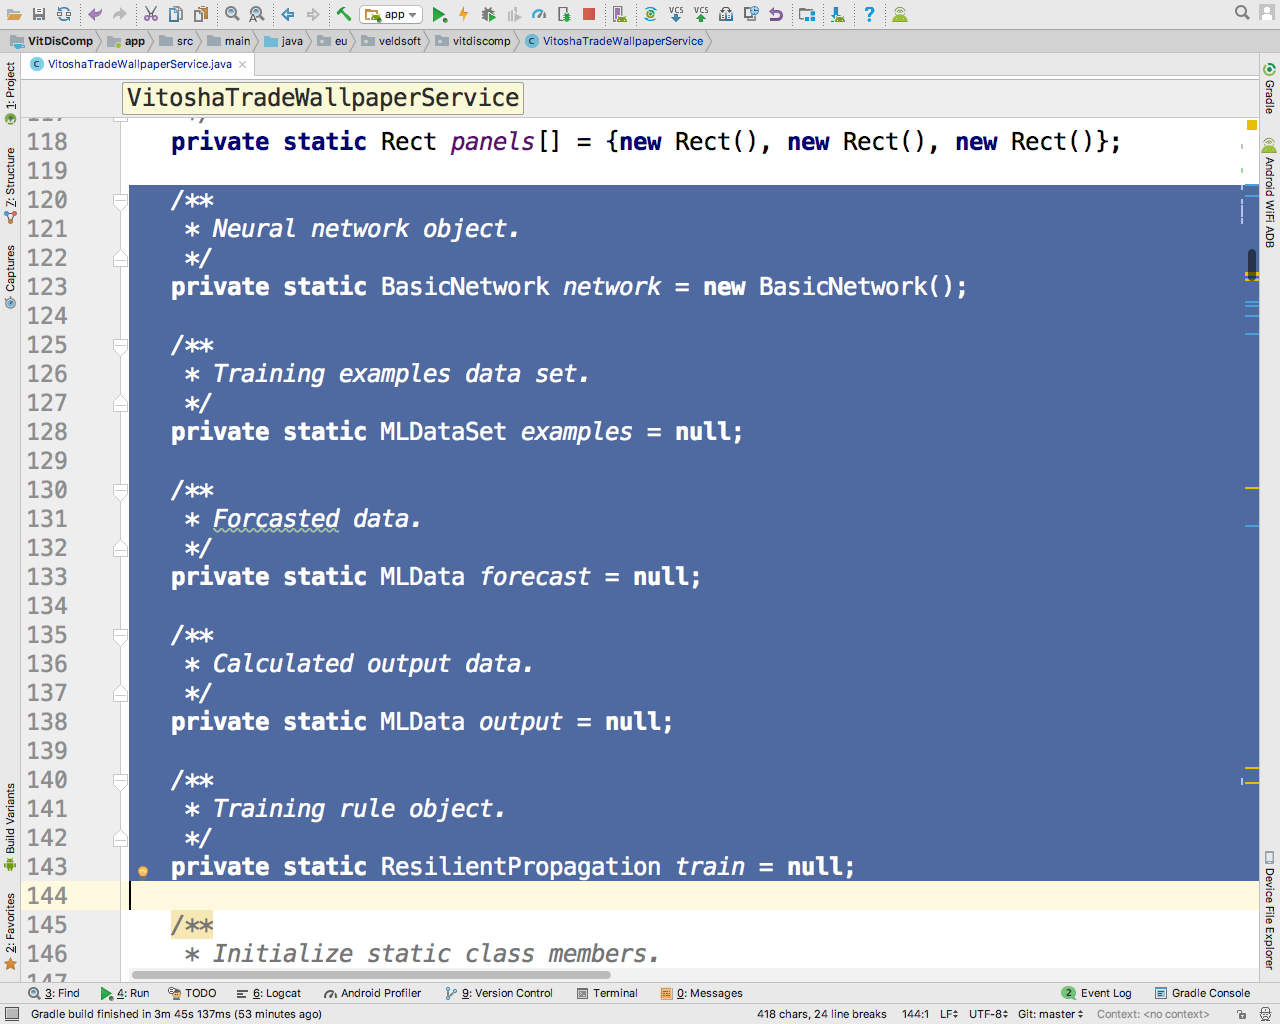
\includegraphics[height=0.45\pdfpageheight]{pic0034}
  \caption{Променливи отговарящи за изкуствената невронна мрежа.}
\label{fig:pic0034}
\end{figure}
\FloatBarrier

При комерсиалното производство на софтуер много често използван похват е създаването на „софтуерни тапи“. Това са парчета код, които служат за комуникация между обекти и части от системата, които още не са създадени. В настоящия случай точно такава софтуерна тапа представя липсата на сървър и източник с реални данни  (Фиг. \ref{fig:pic0035}).  

\begin{figure}[h]
  \centering
  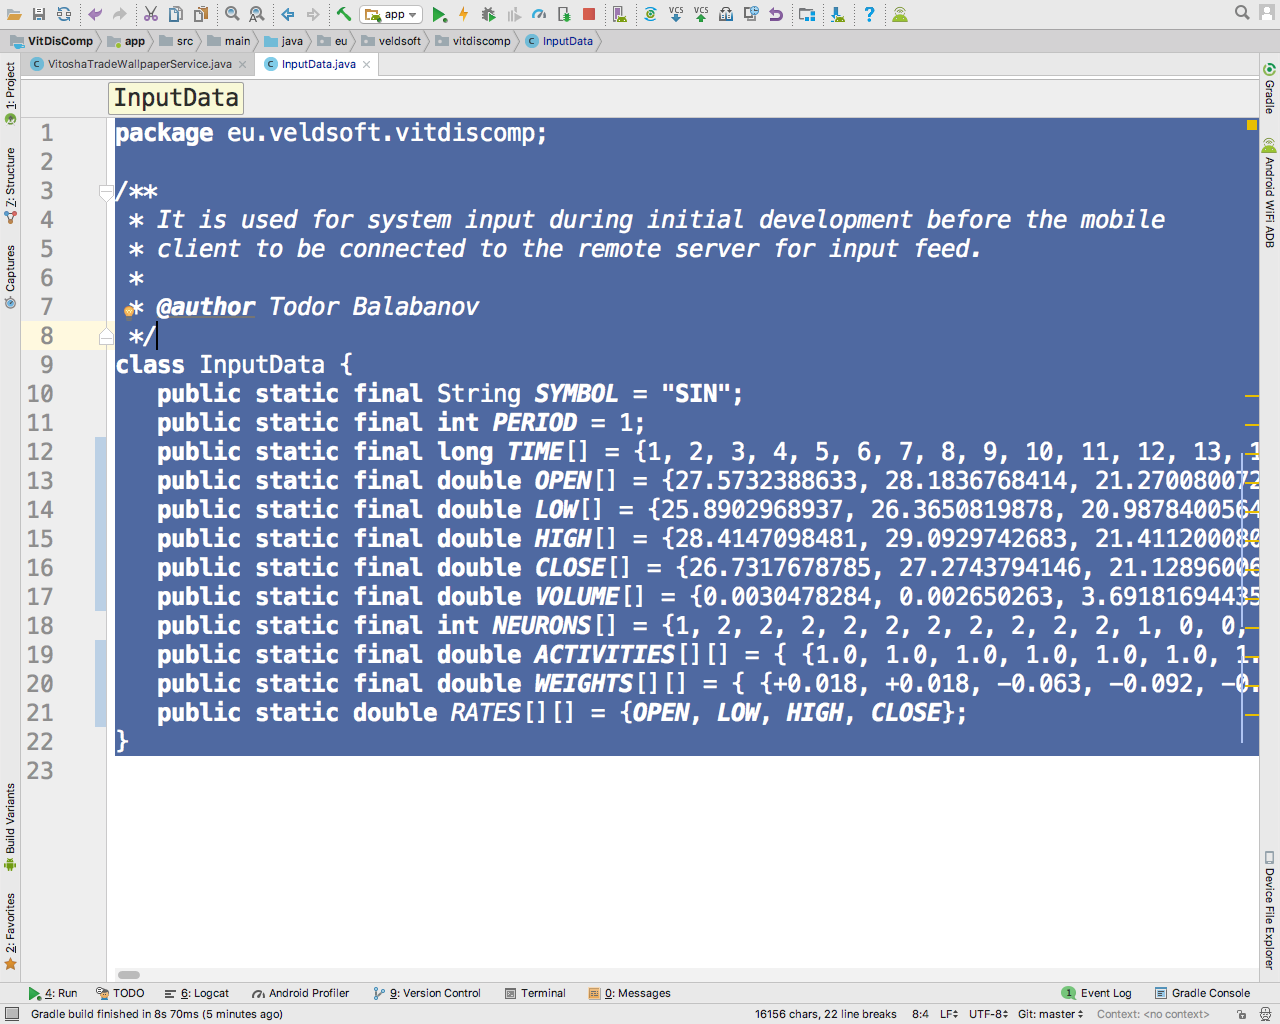
\includegraphics[height=0.45\pdfpageheight]{pic0035}
  \caption{Променливи отговарящи за изкуствената невронна мрежа.}
\label{fig:pic0035}
\end{figure}
\FloatBarrier

Финансовите времеви редове най-често се описват със следните характеристики: 1. Вид финансов инструмент (ticker symbol или stock symbol), в случая математическата функция синус; 2. Интервал между отделните измервания (отчитан в брой минути), в случая една минута; 3. Шест паралелни масива (дискретно време, нива на отваряне, най-ниско постигнато ниво, най-високо постигнато ниво, нива на затваряне и изтъргуван обем).

Освен финансовата информация, към клиентското приложение трябва да се подава и информация за топологията на изкуствената невронна мрежа. За описанието на изкуствената невронна мрежа са нужни: 1. Брой, подредба и тип на невроните (едномерен масив от константи); 2. Матрица на съседство между невроните (единица там където има връзка и нула там където няма връзка); 3. Текуща стойност на тегловния коефициент за всяка връзка между два неврона (включително и примките, ако има такива). 

\begin{figure}[h]
  \centering
  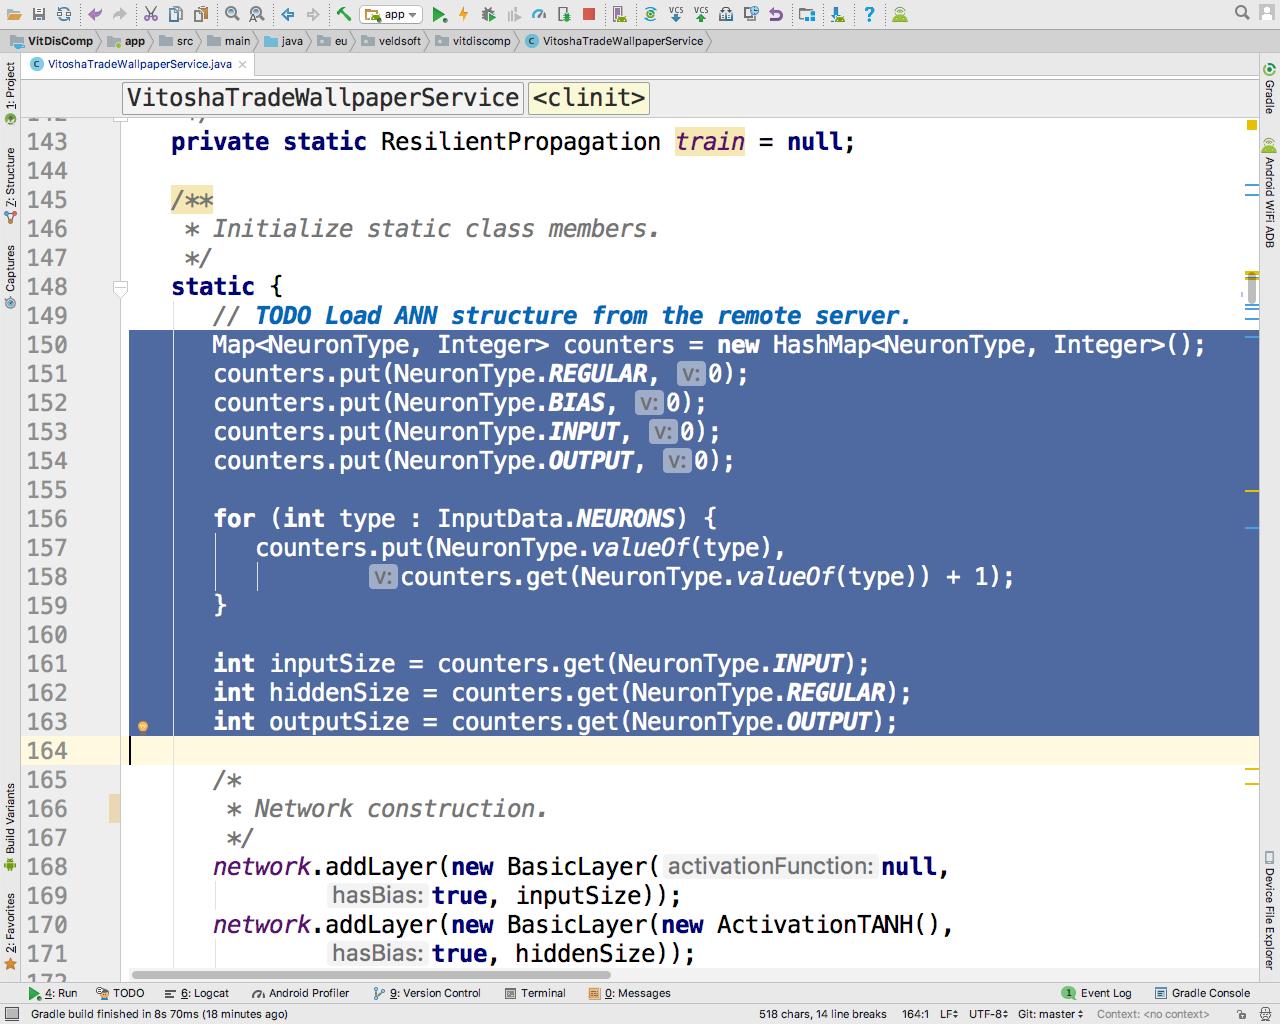
\includegraphics[height=0.45\pdfpageheight]{pic0036}
  \caption{Определяне на броя и типовете неврони.}
\label{fig:pic0036}
\end{figure}
\FloatBarrier

Чрез сортиране с броене ефективно се определя броят на невроните и техните типове (Фиг. \ref{fig:pic0036}).

\begin{figure}[h]
  \centering
  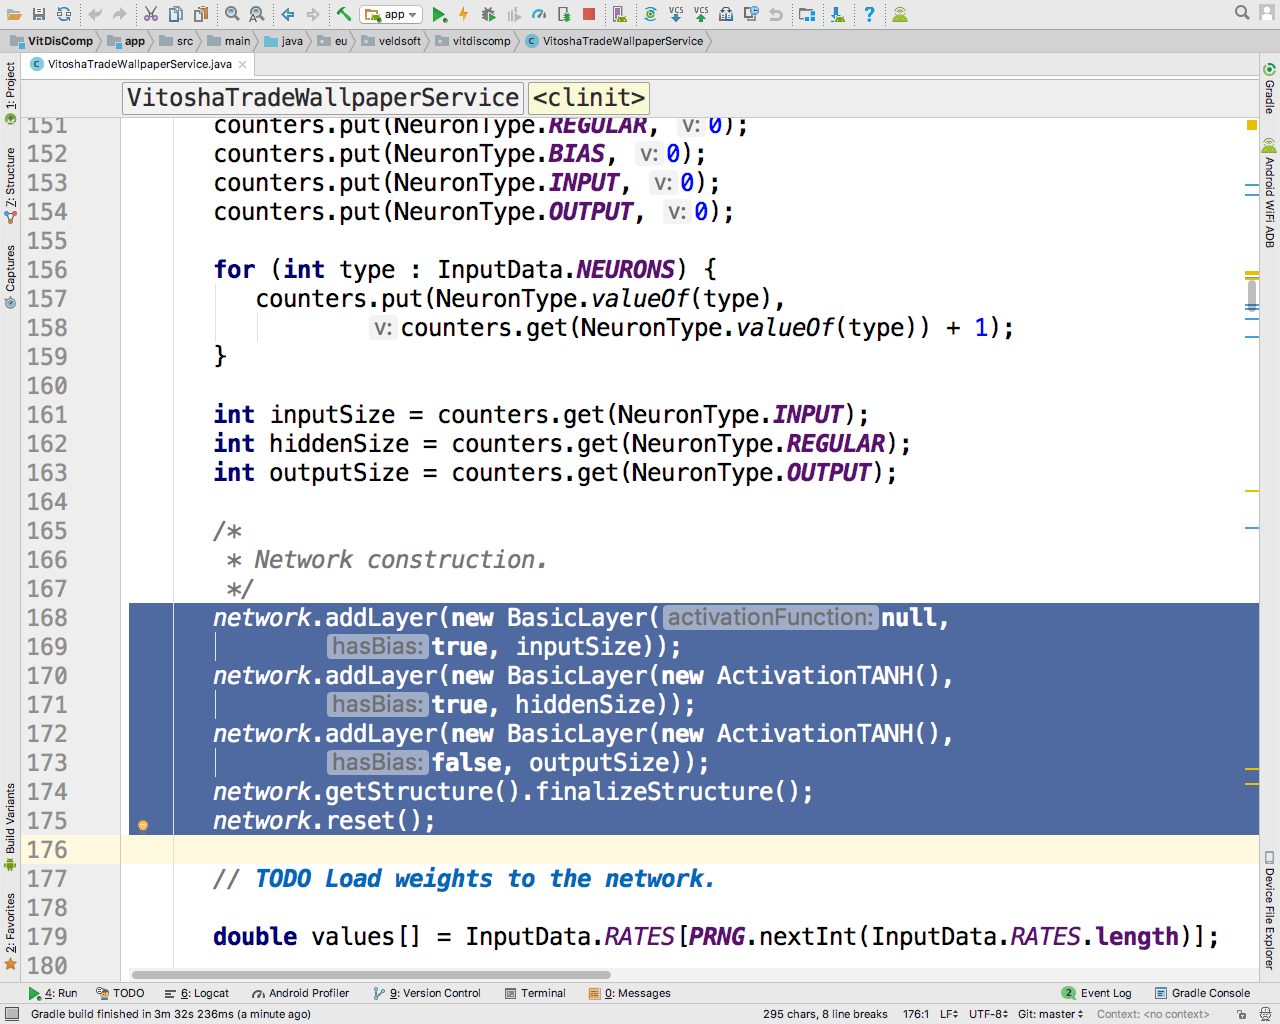
\includegraphics[height=0.45\pdfpageheight]{pic0037}
  \caption{Структура на трислойна изкуствена невронна мрежа.}
\label{fig:pic0037}
\end{figure}
\FloatBarrier

За да се илюстрират възможностите за прогнозиране на изкуствените невронни мрежи е избрана една от най-популярните структури, а именно трислойна невронна мрежа, която се обучава с обратно разпространение на грешката (Фиг. \ref{fig:pic0037}). Входният слой има единствената задача да получи сигналите от външната среда и поради тази причина не се задава активационна функция. За скрия и изходния слой е избрана функцията хиперболичен тангенс, тъй като тя е асимптотично сходима в безкрайностите по абцисата и в същото време е симетрична по същата тази ос. Входния и скрития слой имат отместващ неврон (bias), който не е нужен в изходния слои, тъй като отместващия неврон винаги емитира високото ниво на сигнализация.

\begin{figure}[h]
  \centering
  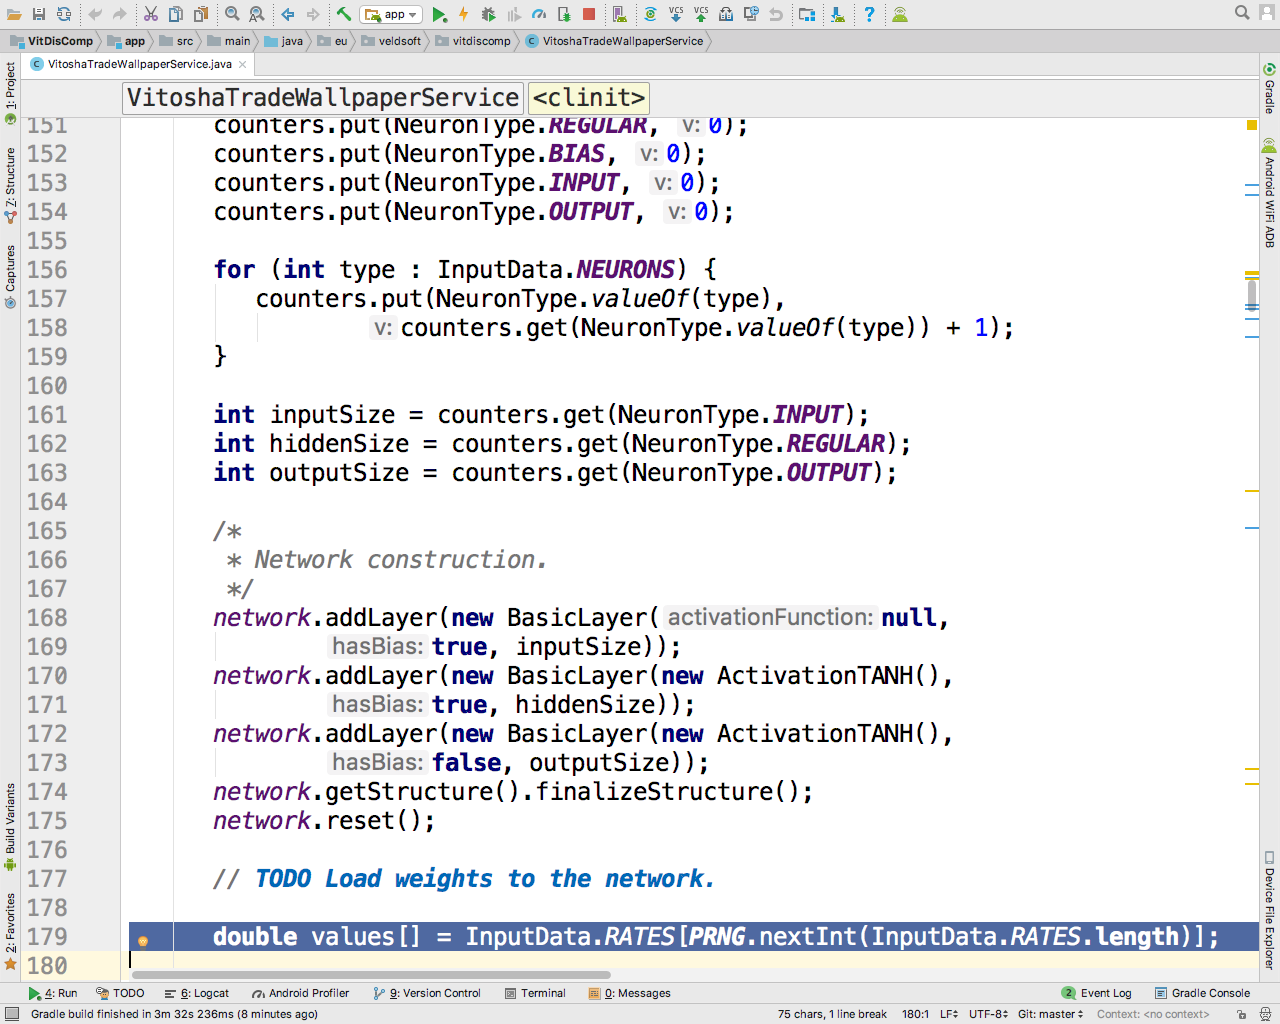
\includegraphics[height=0.45\pdfpageheight]{pic0038}
  \caption{Избор на стойности за прогнозиране.}
\label{fig:pic0038}
\end{figure}
\FloatBarrier

От описанието на паралелните масиви при финансовите времеви редове ясно се вижда, че има четири възможни редици числа, които да се подават за прогнозиране към невронната мрежа (отваряне, най-ниско, най-високо, затваряне). 

\begin{figure}[h]
  \centering
  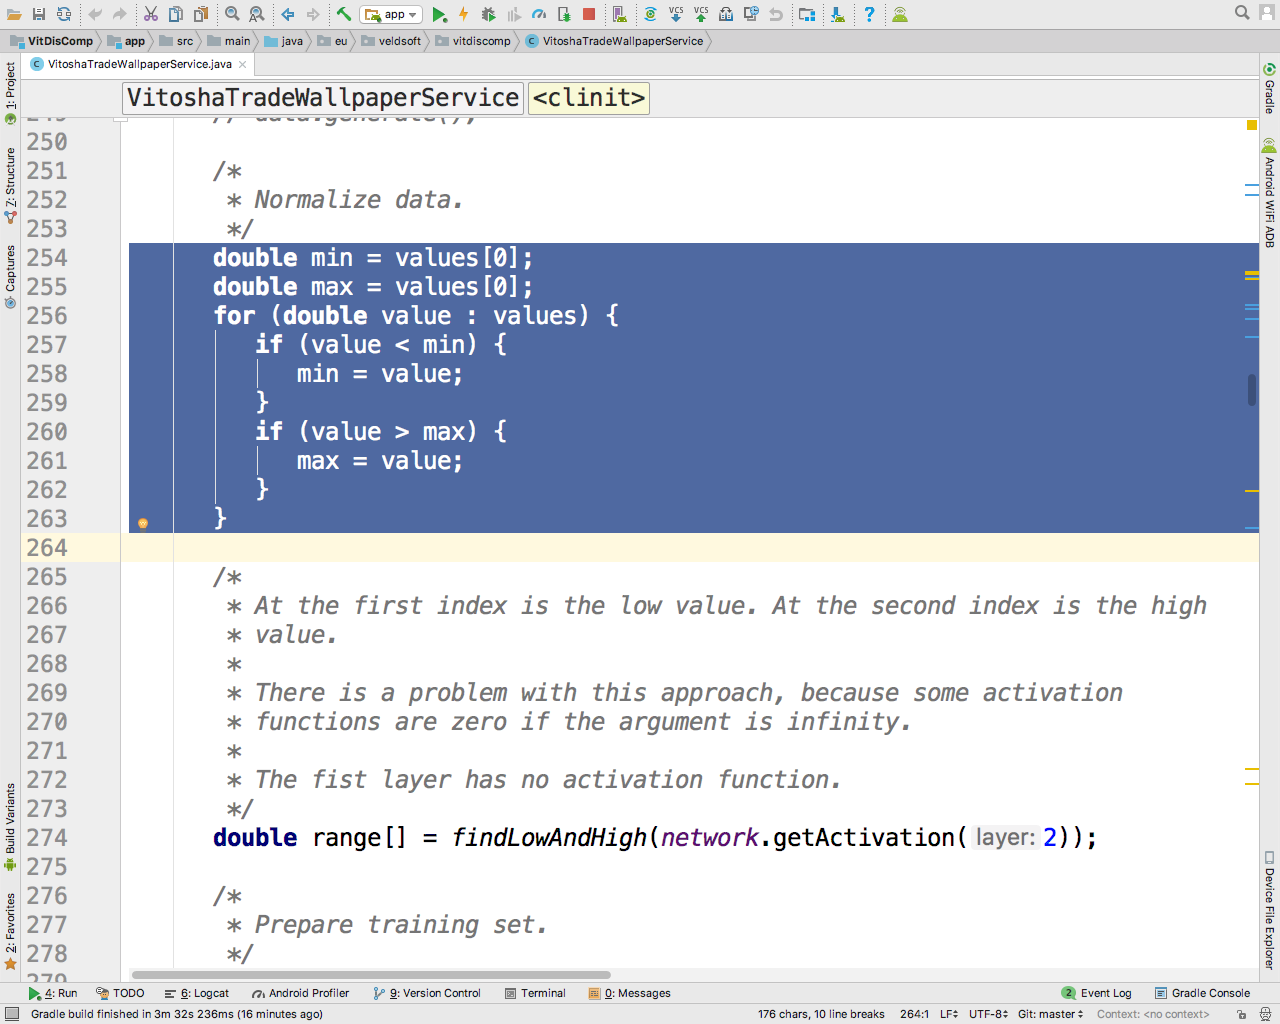
\includegraphics[height=0.45\pdfpageheight]{pic0039}
  \caption{Определяне на границите във времевия ред.}
\label{fig:pic0039}
\end{figure}
\FloatBarrier

В практиката най-често се използва поредицата за стойности на затваряне, а целта е да се прогнозира нивото на отваряне в следващия времеви интервал. Целите на настоящото изложение не са реално постигане на финансови прогнози и поради тази причина на случаен принцип се избира коя последователност да бъде използвана при различните стартирания на обучението/прогнозирането (Фиг. \ref{fig:pic0038}).

\begin{figure}[h]
  \centering
  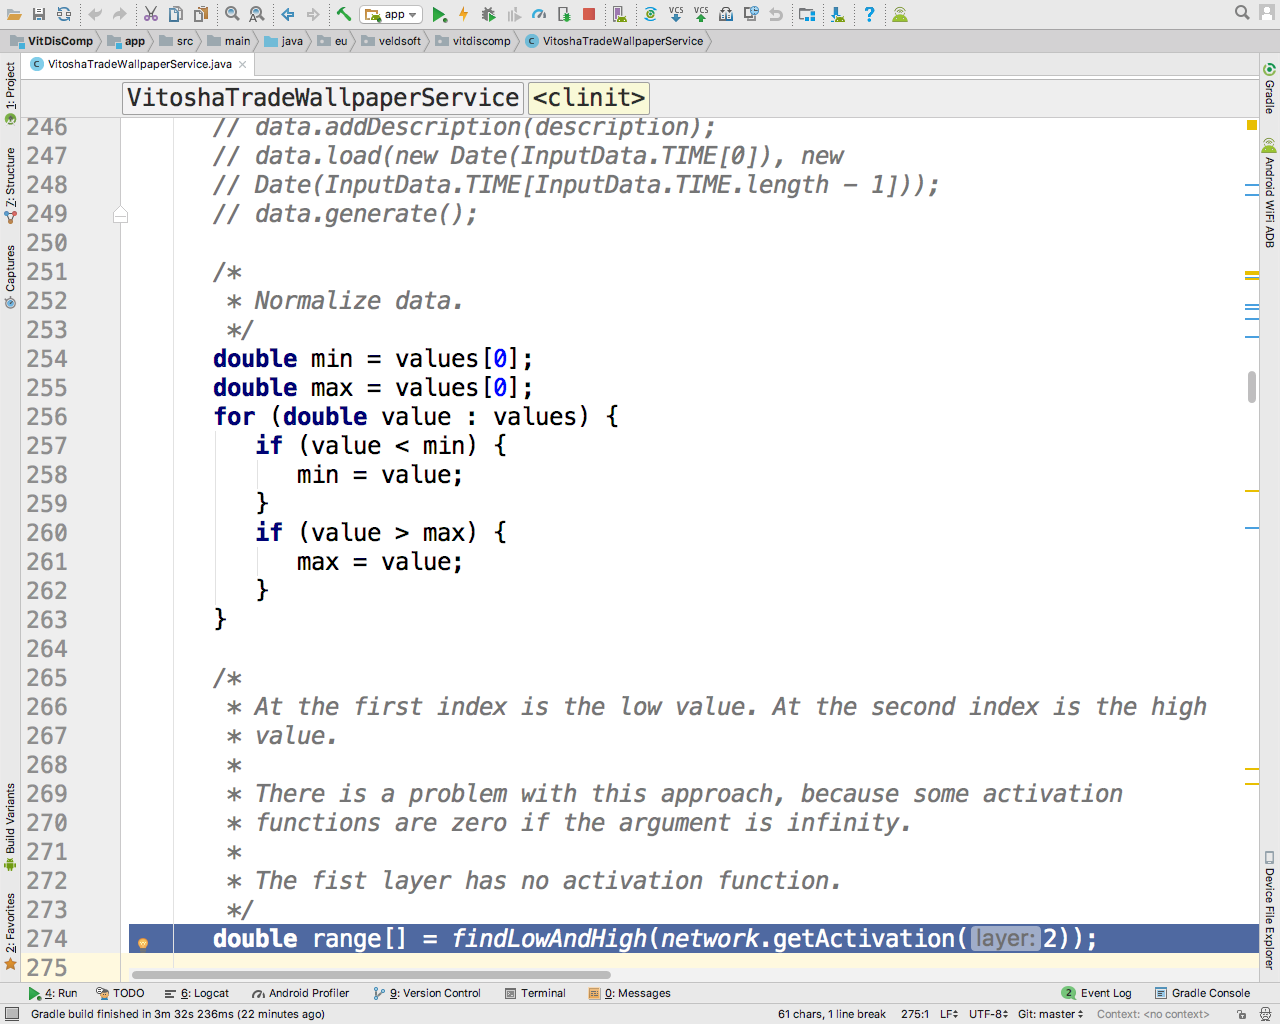
\includegraphics[height=0.45\pdfpageheight]{pic0040}
  \caption{Диапазон на активационната функция в изходния слой.}
\label{fig:pic0040}
\end{figure}
\FloatBarrier

Тъй като целта е към системата за прогнозиране да се подават различни финансови времеви редове то неизбежно се налага входната информация в системата да бъде предварително нормализирана, а първата стъпка към това е да се определят най-големите и най-малките стойности във времевия ред (Фиг. \ref{fig:pic0039}). В същото време данните трябва да бъдат съпоставени на диапазона в който работят активационните функции на изкуствената невронна мрежа. В настоящата разработка е прието, че на входа ще се подадат дигнали в диапазона на функцията използвана в изходния слой (Фиг. \ref{fig:pic0040}). Такова решение се аргументира с факта, че информацията подадена от невронната мрежа към външната среда ще претърпи обратен процес на преоразмеряване, така че да има смисъл в конкретния финансов времеви ред.

\begin{figure}[h]
  \centering
  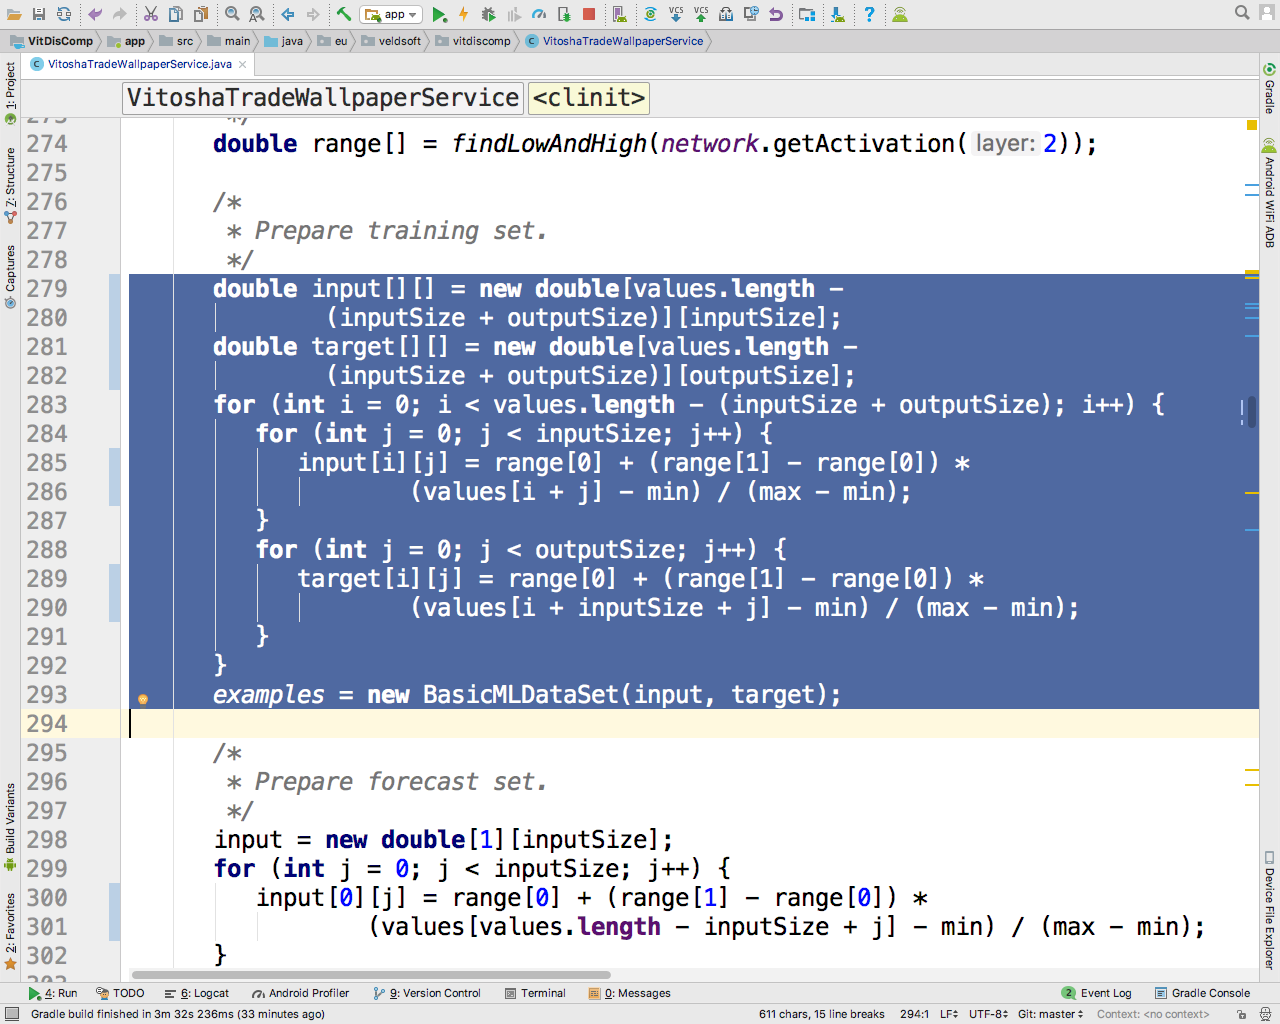
\includegraphics[height=0.45\pdfpageheight]{pic0041}
  \caption{Тренировъчни примери.}
\label{fig:pic0041}
\end{figure}
\FloatBarrier

Нормализираните входни данни условно разделяме на две множества (измервания в миналото и измервания в бъдещето). Разделянето е условно, тъй като практически данните са от реални измервания в миналото (Фиг. \ref{fig:pic0041}).

\begin{figure}[h]
  \centering
  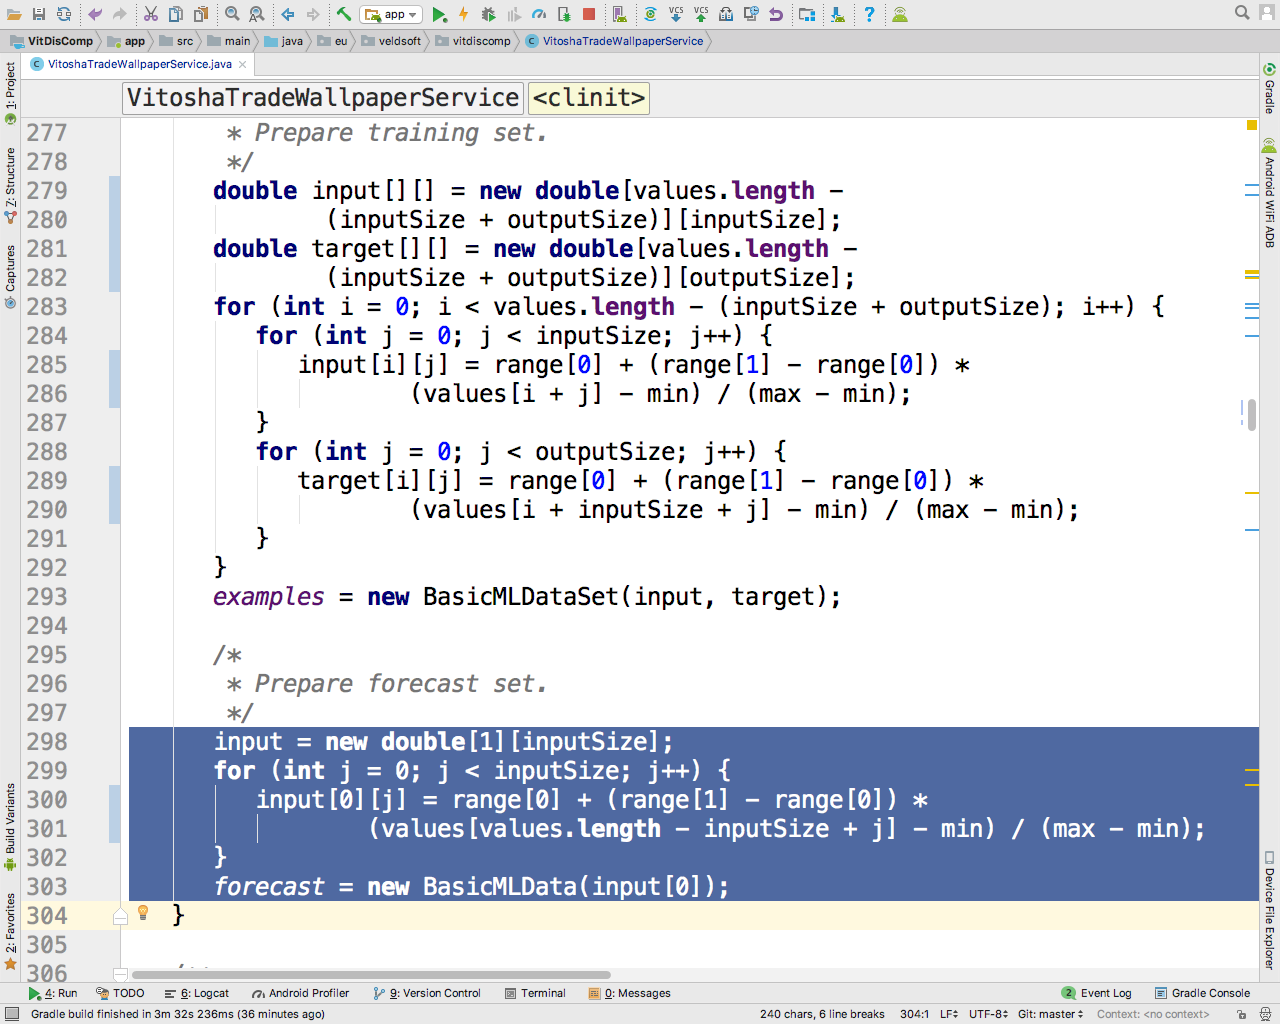
\includegraphics[height=0.45\pdfpageheight]{pic0042}
  \caption{Входни данни към изкуствената неверонна мрежа за получаване на прогноза.}
\label{fig:pic0042}
\end{figure}
\FloatBarrier

Тъй като изкуствената неверонна мрежа се използва и в двата й режима (обучение и прогнозиране) то се изготвя и вектор входни данни, спрямо които да бъде направена прогноза (Фиг. \ref{fig:pic0042}).

\begin{figure}[h]
  \centering
  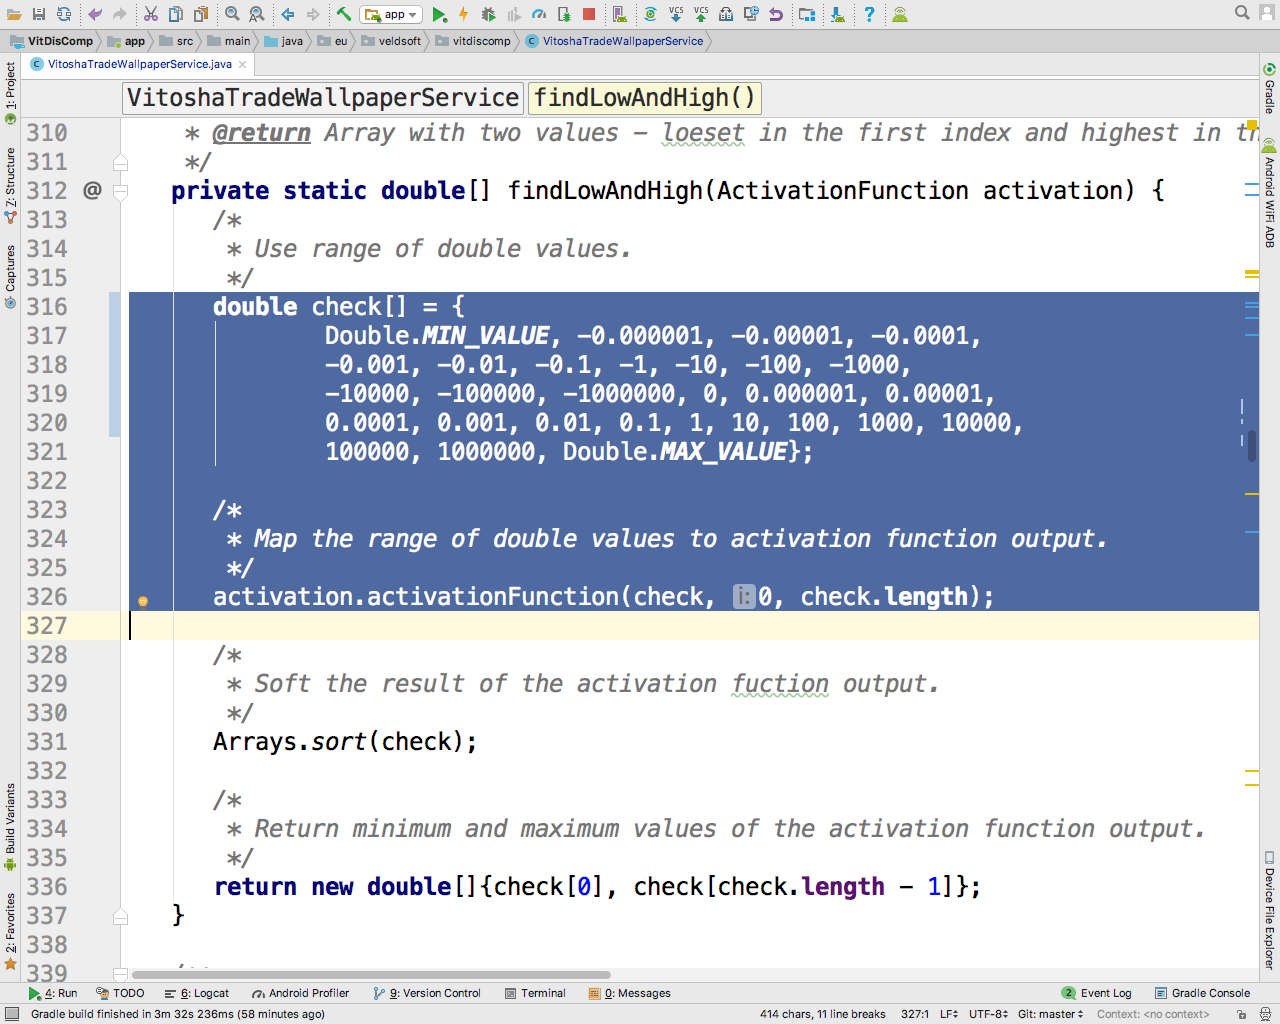
\includegraphics[height=0.45\pdfpageheight]{pic0043}
  \caption{Изследване на група от стойности за определяне на диапазона.}
\label{fig:pic0043}
\end{figure}
\FloatBarrier

В общия случай активационните функции имат асимптотична сходимост и са монотонно нарастващи (Фиг. \ref{fig:pic0044}), което позволява техните крайни диапазони да бъдат установявани, чрез проверка на група от стойности (Фиг. \ref{fig:pic0043}).

\begin{figure}[h]
  \centering
  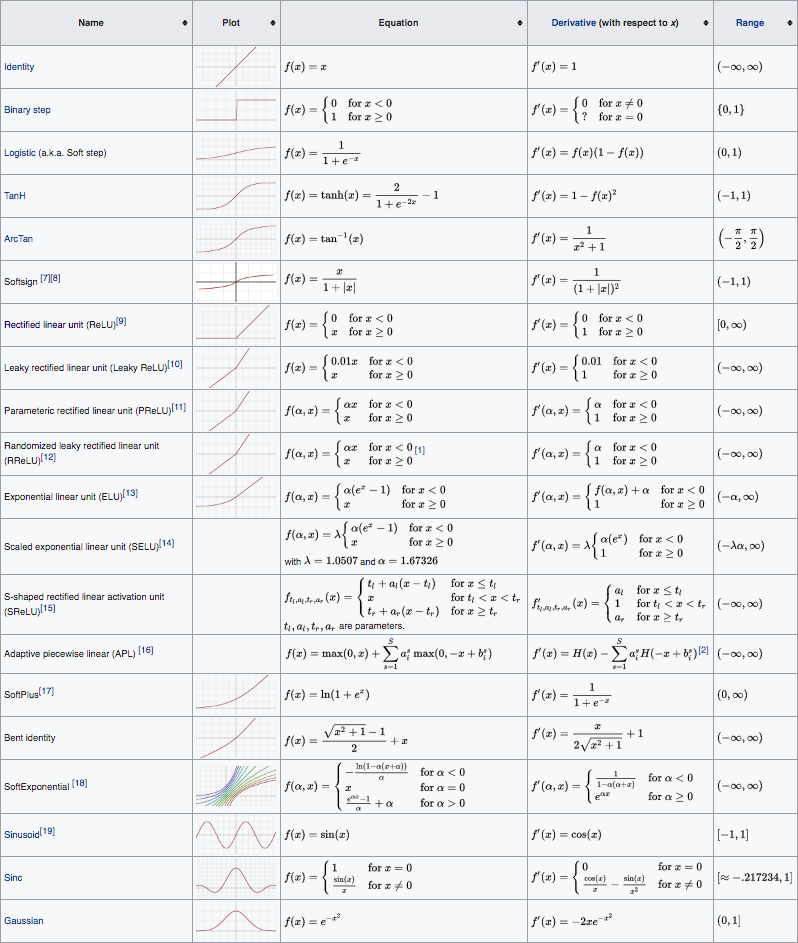
\includegraphics[height=0.7\pdfpageheight]{pic0044}
  \caption{Активационни функции \cite{afwiki}.}
\label{fig:pic0044}
\end{figure}
\FloatBarrier

Както е добре видно на Фиг. \ref{fig:pic0044}, за някои от активационните функции такова определяне на диапазона може да се окаже силно подвеждащо (примерно при синус функцията). 

\begin{figure}[h]
  \centering
  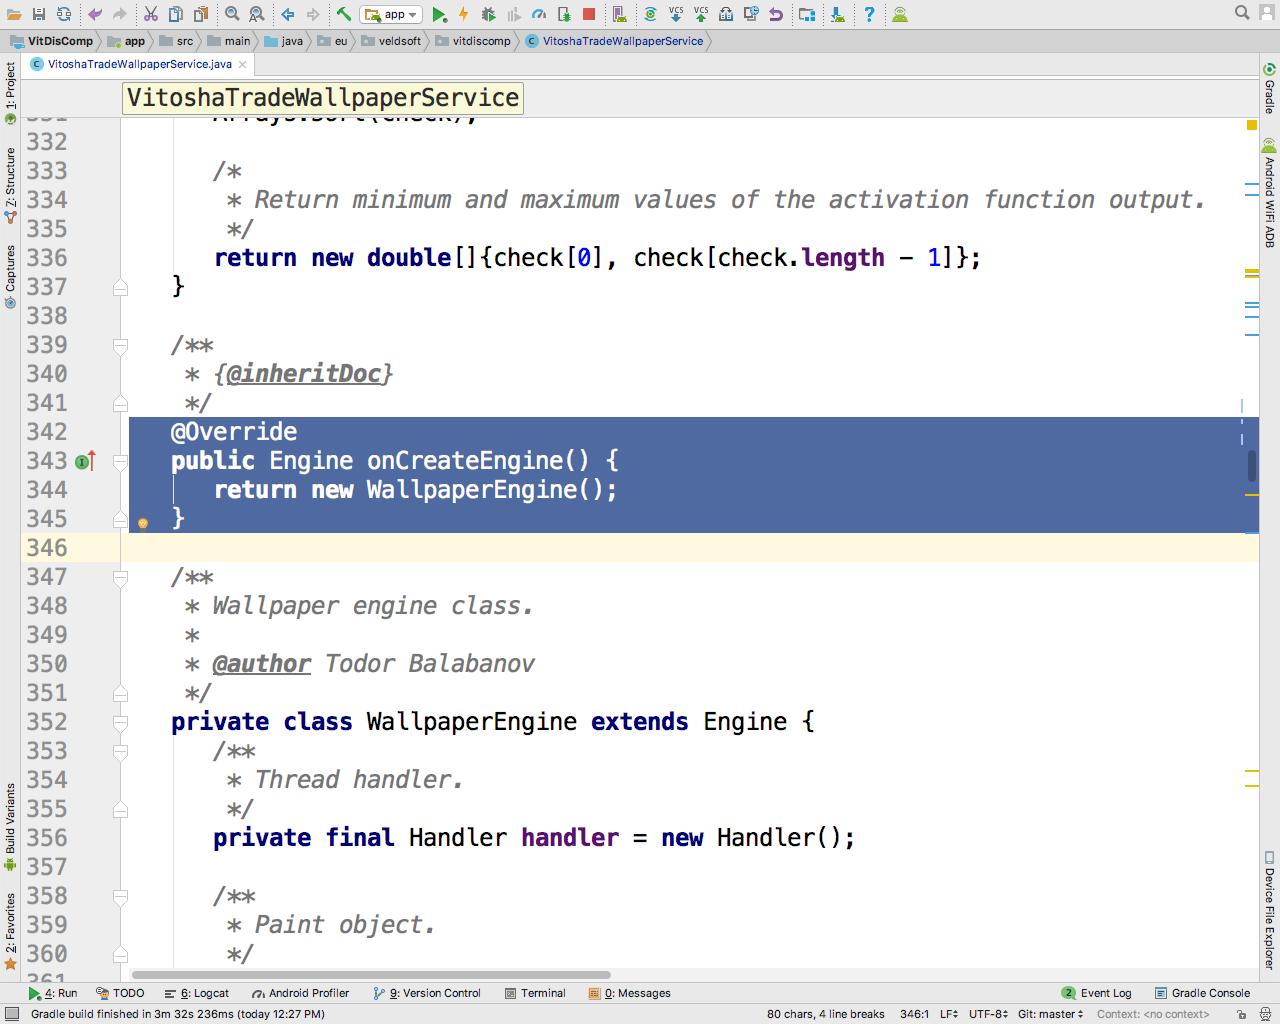
\includegraphics[height=0.45\pdfpageheight]{pic0045}
  \caption{Собствен engine обект.}
\label{fig:pic0045}
\end{figure}
\FloatBarrier

Събитието за създаване на engine обект се предефинира, така че да се връща обект от нашия собствен клас за engine (Фиг. \ref{fig:pic0045}). 

\section{Двигател на услугата}

Същинската работа за фоново пресмятане в услугата се извършва от обект описан с частен вътрешен клас от тип „двигател“ (Engine).

\begin{figure}[h]
  \centering
  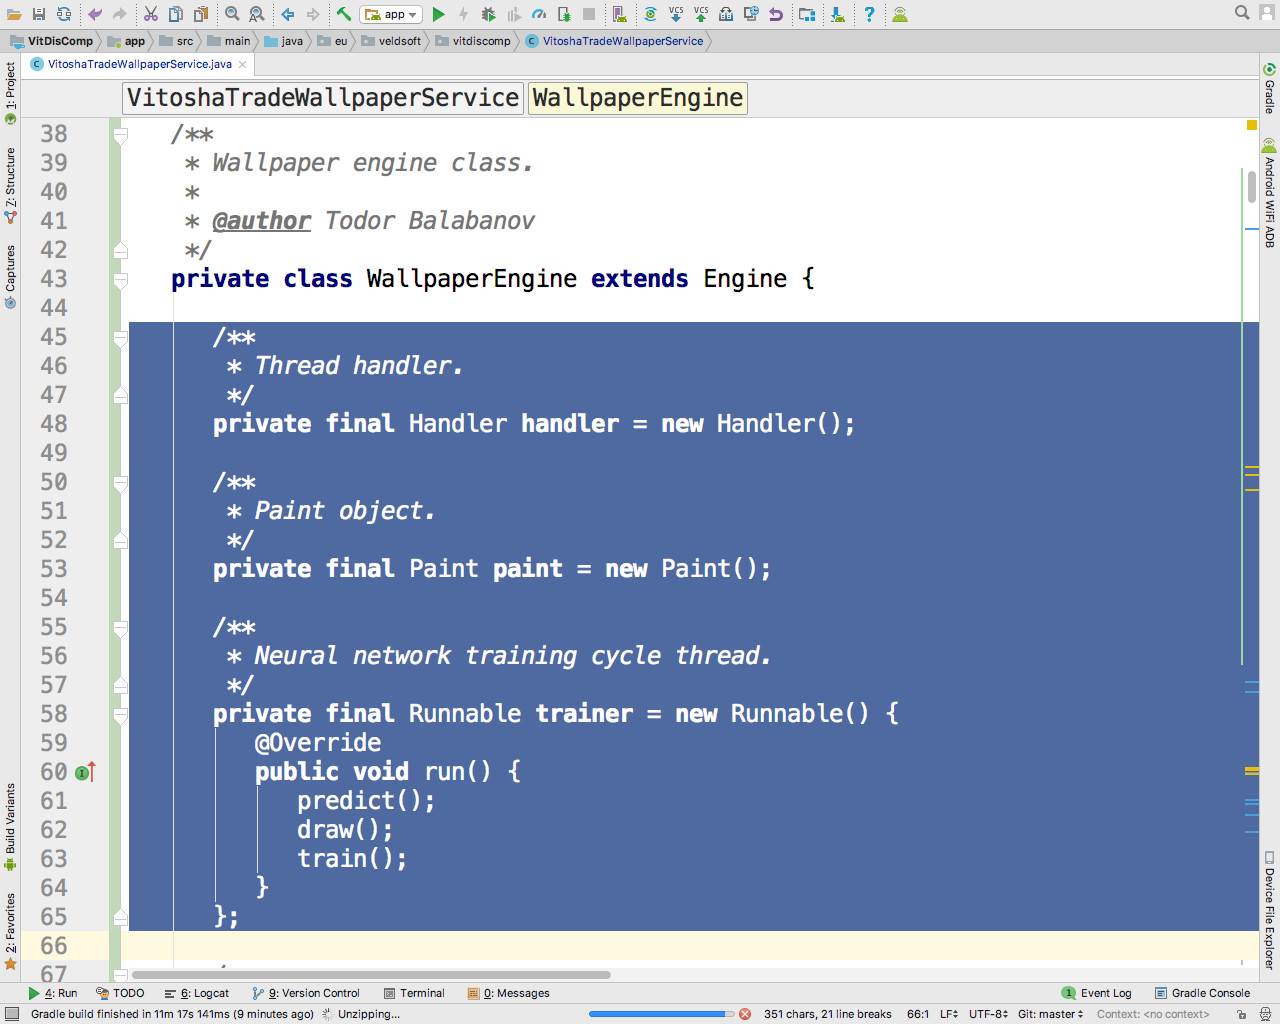
\includegraphics[height=0.45\pdfpageheight]{pic0046}
  \caption{Вътрешни променливи за двигателя на услугата.}
\label{fig:pic0046}
\end{figure}
\FloatBarrier

В този двигател се използват три вътрешни променливи (Фиг. \ref{fig:pic0046}). Обектът от тип „четка“ (Paint) е само спомагателен и служи за еднократно определяне на характеристиките за изрисуване. Ползата е, че обекта бива създаден веднъж и след това се ползва през целия жизнен цикъл на услугата. 

\begin{figure}[h]
  \centering
  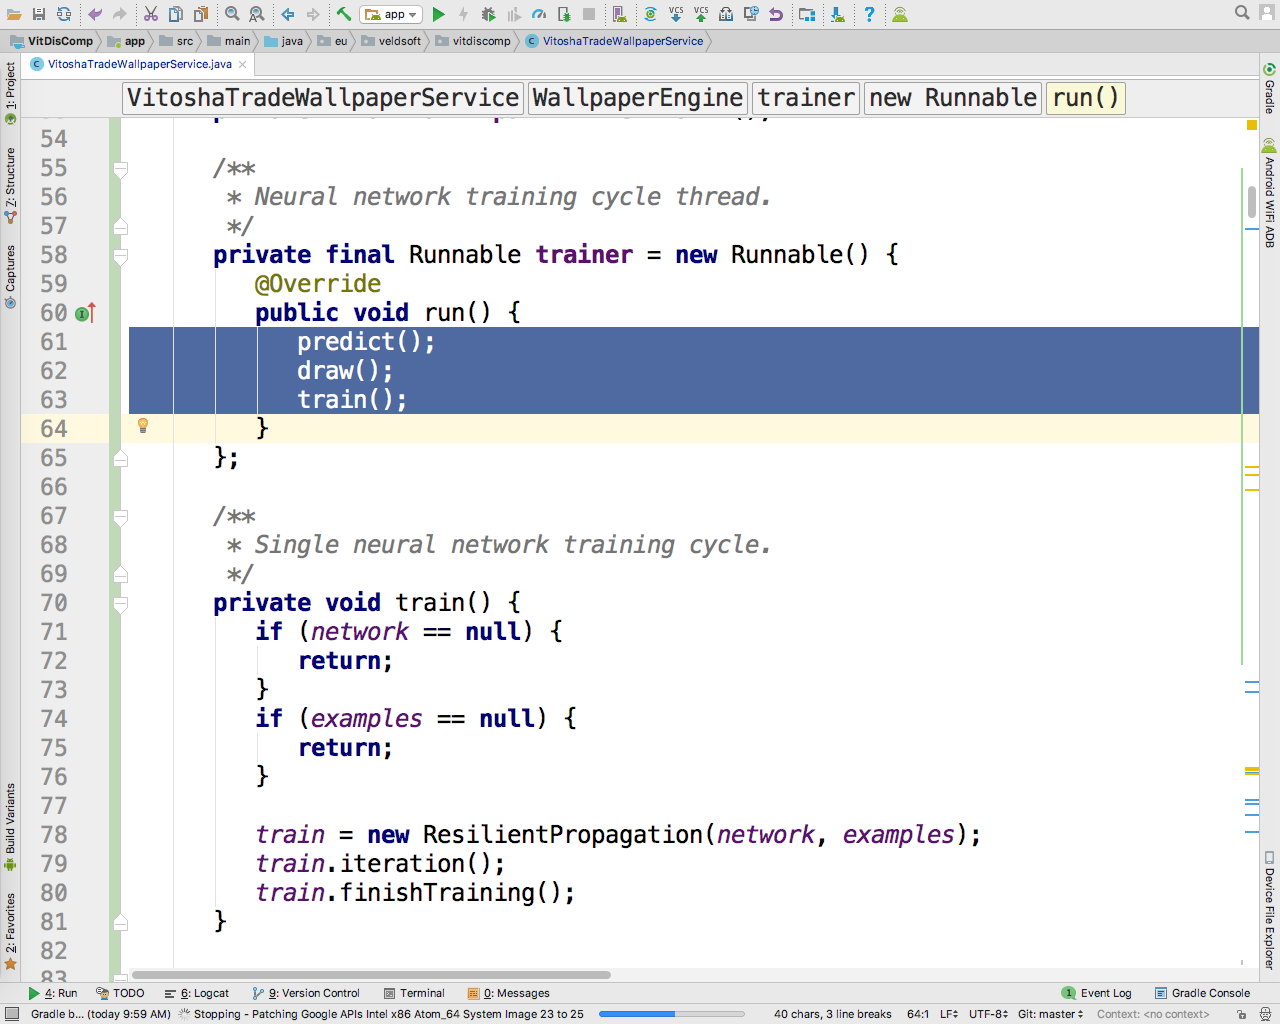
\includegraphics[height=0.45\pdfpageheight]{pic0047}
  \caption{Единичен цикъл във фонов режим.}
\label{fig:pic0047}
\end{figure}
\FloatBarrier

За реалната работа на двигателя се дефинира отделна нишка (trainer) която да извършва операциите по генериране на прогноза, изчертаване на активния тапет и извършването на един цикъл от обучаващия процес на изкуствената невронна мрежа\index{изкуствени невронни мрежи} (Фиг. \ref{fig:pic0047}). Ефективното управление на нишки в Android се извършва с помощта на обекти „държател“ (Handler). Обектът държател поема отговорността по стартирането на нишката, спирането на нишката и реализацията на интервала за изчакване преди да бъде осъществено следващото събуждане на нишката. 

\begin{figure}[h]
  \centering
  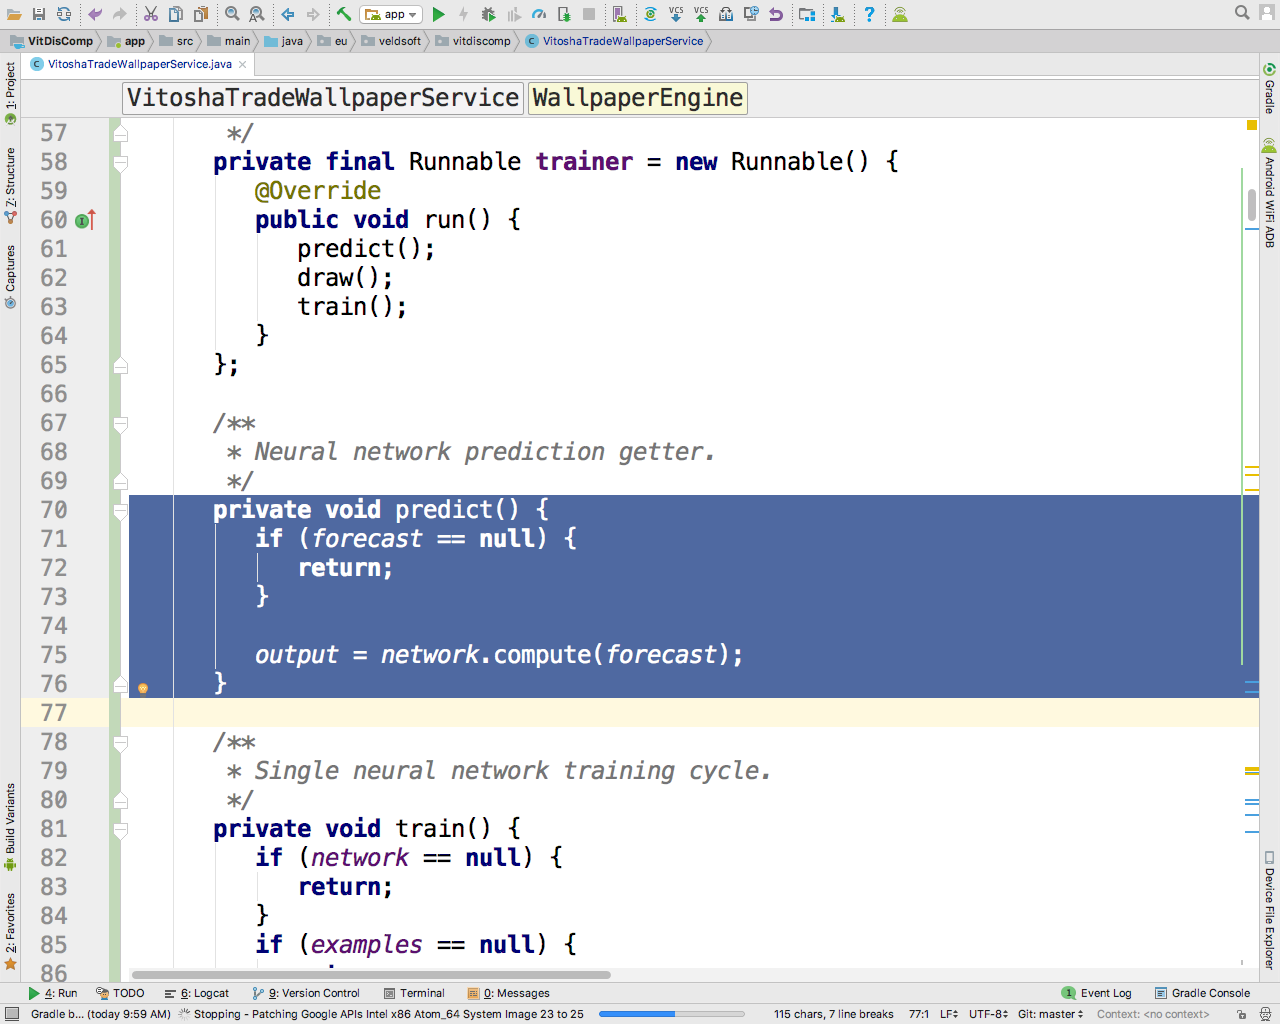
\includegraphics[height=0.45\pdfpageheight]{pic0048}
  \caption{Изчисляване на прогноза.}
\label{fig:pic0048}
\end{figure}
\FloatBarrier

За да се изчисли прогноза, според текущото ниво на обученост на изкуствената невронна мрежа\index{изкуствени невронни мрежи}, е достатъчно мрежата да се активира в работен режим с подходящи данни към входния слой (Фиг. \ref{fig:pic0048}).

\begin{figure}[h]
  \centering
  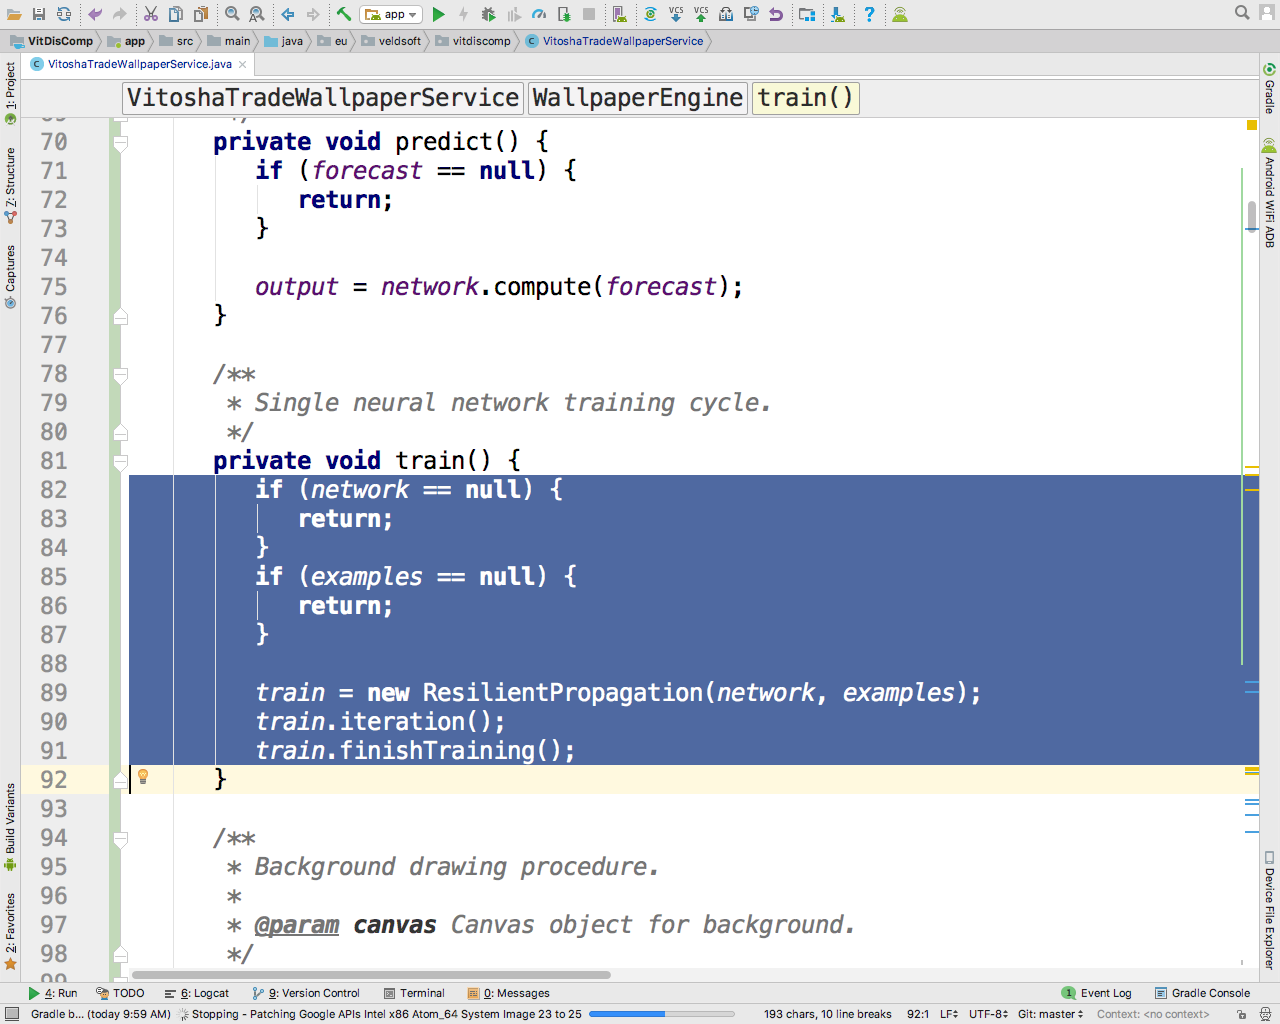
\includegraphics[height=0.45\pdfpageheight]{pic0049}
  \caption{Тренировъчен цикъл на изкуствената невронна мрежа.}
\label{fig:pic0049}
\end{figure}
\FloatBarrier

За да се осъществи един тренировъчен цикъл на изкуствената невронна мрежа\index{изкуствени неверонни мрежи} е достатъчно да се създаде тренировъчен обект (в случая от еластично обратно разпространение на грешката\index{обратно разпространение на грешката}), към който се подават мрежата и тренировъчните примери (Фиг. \ref{fig:pic0049}).

\begin{figure}[h]
  \centering
  \includegraphics[height=0.45\pdfpageheight]{pic0050}
  \caption{Основна процедура по изрисуване на информацията от тренировъчния процес.}
\label{fig:pic0050}
\end{figure}
\FloatBarrier

Изрисуването на информацията от тренировъчния процес е организирано в отделна функция (Фиг. \ref{fig:pic0050}). За да бъде осъществена визуализацията се осигурява достъп до повърхността и платното което тя съдържа. В самия край на функцията за визуализация се взема решение дали ще се изпълни следващ цикъл на обучение или изпълнението ще бъде преустановено. 

\begin{figure}[h]
  \centering
  \includegraphics[height=0.45\pdfpageheight]{pic0051}
  \caption{Разбиване на задачата за визуализация.}
\label{fig:pic0051}
\end{figure}
\FloatBarrier

Добрите практики за писане на програмен код включват разбиване на една сложна задача в група от множество по-прости задачи. Този принцип е приложен по отношение на визуализацията, като са създадени пет помощни функции (Фиг. \ref{fig:pic0051}).  Първата функция изрисува фон, втората очертава полупрозрачни области за панелите, третата запълва панела с информация за валутната двойка, четвъртата показва информация в панела за текущо актуалната прогноза, а петата стилизиран модел на изкуствената неверонна мрежа\index{изкуствени невронни мрежи}. 

\begin{figure}[h]
  \centering
  \includegraphics[height=0.45\pdfpageheight]{pic0052}
  \caption{Изрисуване на фона.}
\label{fig:pic0052}
\end{figure}
\FloatBarrier

За да бъде изрисуван фона се зарежда предварително подготвено изображение и от него се отрязва такова парче, че да пасва на размерите на екрана (Фиг. \ref{fig:pic0052}). Коя част от изображението да бъде използвана се определя на случаен принцип.

\begin{figure}[h]
  \centering
  \includegraphics[height=0.45\pdfpageheight]{pic0053}
  \caption{Изрисуване на областите за служебна информация.}
\label{fig:pic0053}
\end{figure}
\FloatBarrier

Веднага след изрисуването на фона се изрисуват и полупрозрачните петна за визуализация на информацията от процеса по обучението (Фиг. \ref{fig:pic0053}). Похватът за полупрозрачност е нужен за да се избегне страничният ефект от сливане на цветове между служебната информация и фона. 

\begin{figure}[h]
  \centering
  \includegraphics[height=0.45\pdfpageheight]{pic0054}
  \caption{Изрисуване на информацията за валутната двойка.}
\label{fig:pic0054}
\end{figure}
\FloatBarrier

Информацията за валутната двойка се състои от название и времеви интервал на финансовия времеви ред (Фиг. \ref{fig:pic0054}). 

\begin{figure}[h]
  \centering
  \includegraphics[height=0.45\pdfpageheight]{pic0055}
  \caption{Позиция и размери за визуализация на прогнозата.}
\label{fig:pic0055}
\end{figure}
\FloatBarrier

Визуализацията на прогнозата изисква малко по-сложни пресмятания, така че информацията от входа и изхода да се поместят в рамките на определеното петно. За да бъде изпълнена тази задача се вземат координатите и размерите на определената област (Фиг. \ref{fig:pic0055}). 

\begin{figure}[h]
  \centering
  \includegraphics[height=0.45\pdfpageheight]{pic0056}
  \caption{Обхват на данните по ширина и височина.}
\label{fig:pic0056}
\end{figure}
\FloatBarrier

За да бъдат визуализирани данните е от съществено значение да се определи минималната и максимална стойност за вход-изхода, както и броя стойности, които ще бъдат визуализирани (Фиг. \ref{fig:pic0056}). В случая броя стойности за визуализация съвпада със сумата от броя входни въздействия и броя изходни сигнали. 

\begin{figure}[h]
  \centering
  \includegraphics[height=0.45\pdfpageheight]{pic0057}
  \caption{Цикли за визуализация на стълбовете от времевия реди и прогнозата.}
\label{fig:pic0057}
\end{figure}
\FloatBarrier

Данните за отминалия период от време се показват с един цвят, а данните за прогнозата в друг цвят (Фиг. \ref{fig:pic0057}). Самата визуализация представлява bar-chart на входните данни и на прогнозата. 

\begin{figure}[h]
  \centering
  \includegraphics[height=0.45\pdfpageheight]{pic0058}
  \caption{Топология на изкуствената невронна мрежа която се визуализира.}
\label{fig:pic0058}
\end{figure}
\FloatBarrier

В третата област за визуализация се изрисува стилизирана информация за състоянието на изкуствената невронна мрежа\index{изкуствени неверонни мрежи}. Областта е правоъгълна и бива разделена на пет вертикални зони: 1. Стойности на невроните във входния слой; 2. Стойности на теглата между входния и скрития слой; 3. Стойности на невроните в скрития слой; 4. Стойности на теглата между скрития и изходния слой; 5. Стойности на невроните в изходния слой (Фиг. \ref{fig:pic0058}).

\begin{figure}[h]
  \centering
  \includegraphics[height=0.45\pdfpageheight]{pic0059}
  \caption{Мащабиране на входната и изходната информация.}
\label{fig:pic0059}
\end{figure}
\FloatBarrier

Информацията за входа и изхода се преоразмерява спрямо минималните и максималните стойности с които работят невроните в изходния слой (Фиг. \ref{fig:pic0059}). Невроните във входния слой на практика не би трябвало да имат ограничение от активационна функция, тъй като те само събират информацията от външния свят. 

\begin{figure}[h]
  \centering
  \includegraphics[height=0.45\pdfpageheight]{pic0060}
  \caption{Стойности на теглата между слоевете.}
\label{fig:pic0060}
\end{figure}
\FloatBarrier

Следва определянето на теглата между слоевете (Фиг. \ref{fig:pic0060}).

\begin{figure}[h]
  \centering
  \includegraphics[height=0.45\pdfpageheight]{pic0061}
  \caption{Мащабиране на стойностите в скрития слой.}
\label{fig:pic0061}
\end{figure}
\FloatBarrier

И финално за средната вертикална област се определят стойностите за скрития слой, мащабирани спрямо минималното и максималното ниво на активационната функция приложена в него (Фиг. \ref{fig:pic0061}).

\begin{figure}[h]
  \centering
  \includegraphics[height=0.45\pdfpageheight]{pic0062}
  \caption{Нормализиране на стойностите за теглата.}
\label{fig:pic0062}
\end{figure}
\FloatBarrier

За да бъде визуализирана информацията за теглата е нужно стойностите им да се нормализират, спрямо най-малката и най-голямата стойност измежду тях (Фиг. \ref{fig:pic0062}).

\begin{figure}[h]
  \centering
  \includegraphics[height=0.45\pdfpageheight]{pic0063}
  \caption{Изрисуване на топологията.}
\label{fig:pic0063}
\end{figure}
\FloatBarrier

Така подготвените предварително данни с лекота биват визуализирани от група вложение цикли (Фиг. \ref{fig:pic0063}).

\begin{figure}[h]
  \centering
  \includegraphics[height=0.45\pdfpageheight]{pic0064}
  \caption{Конструктор на двигателя за услугата.}
\label{fig:pic0064}
\end{figure}
\FloatBarrier

Конструкторът за двигателя на услугата има единствената задача да зареди нишката за изпълнение (Фиг. \ref{fig:pic0064}).

\begin{figure}[h]
  \centering
  \includegraphics[height=0.45\pdfpageheight]{pic0065}
  \caption{Промяна във видимостта на активния тапет.}
\label{fig:pic0065}
\end{figure}
\FloatBarrier

Когато видимостта на активния тапет бъде променена се активира събитие onVisibilityChanged в което се определя дали нишката да бъде активирана отново или викането й да бъде преустановено (Фиг. \ref{fig:pic0065}).

\begin{figure}[h]
  \centering
  \includegraphics[height=0.45\pdfpageheight]{pic0066}
  \caption{Спиране на пресмятанията при разрушаване на повърхността за изрисуване.}
\label{fig:pic0066}
\end{figure}
\FloatBarrier

При събитие за унищожаване на рисувателната площ бива вдигнат флаг за спиране на изчисленията и нишката отговорна за тях се премахва от опашката за изпълнение (Фиг. \ref{fig:pic0066}).

\begin{figure}[h]
  \centering
  \includegraphics[height=0.45\pdfpageheight]{pic0067}
  \caption{Размер на зоните за изрисуване.}
\label{fig:pic0067}
\end{figure}
\FloatBarrier

Когато настъпи промяна в площта за изрисуване на активния тапет е нужно да се вземат серия мерки по преизчисляване на размерите. Такова събитие примерно настъпва когато устройството сменя визуализацията от портретна в пейзажна или обратното. Първата характеристика която се следи е размерът на петната за визуализация (Фиг. \ref{fig:pic0067}).


\begin{figure}[h]
  \centering
  \includegraphics[height=0.45\pdfpageheight]{pic0068}
  \caption{Координати и размери на областите за визуализация - горе-ляво.}
\label{fig:pic0068}
\end{figure}
\FloatBarrier

\begin{figure}[h]
  \centering
  \includegraphics[height=0.45\pdfpageheight]{pic0069}
  \caption{Координати и размери на областите за визуализация - горе-център.}
\label{fig:pic0069}
\end{figure}
\FloatBarrier

\begin{figure}[h]
  \centering
  \includegraphics[height=0.45\pdfpageheight]{pic0070}
  \caption{Координати и размери на областите за визуализация - горе-дясно.}
\label{fig:pic0070}
\end{figure}
\FloatBarrier

\begin{figure}[h]
  \centering
  \includegraphics[height=0.45\pdfpageheight]{pic0071}
  \caption{Координати и размери на областите за визуализация - център-ляво.}
\label{fig:pic0071}
\end{figure}
\FloatBarrier

\begin{figure}[h]
  \centering
  \includegraphics[height=0.45\pdfpageheight]{pic0072}
  \caption{Координати и размери на областите за визуализация - център-център.}
\label{fig:pic0072}
\end{figure}
\FloatBarrier

\begin{figure}[h]
  \centering
  \includegraphics[height=0.45\pdfpageheight]{pic0073}
  \caption{Координати и размери на областите за визуализация - център-дясно.}
\label{fig:pic0073}
\end{figure}
\FloatBarrier

\begin{figure}[h]
  \centering
  \includegraphics[height=0.45\pdfpageheight]{pic0074}
  \caption{Координати и размери на областите за визуализация - долу-ляво.}
\label{fig:pic0074}
\end{figure}
\FloatBarrier

\begin{figure}[h]
  \centering
  \includegraphics[height=0.45\pdfpageheight]{pic0075}
  \caption{Координати и размери на областите за визуализация - долу-център.}
\label{fig:pic0075}
\end{figure}
\FloatBarrier

\begin{figure}[h]
  \centering
  \includegraphics[height=0.45\pdfpageheight]{pic0076}
  \caption{Координати и размери на областите за визуализация - долу-дясно.}
\label{fig:pic0076}
\end{figure}
\FloatBarrier

На потребителя е позволено да избере в коя част на активния тапет да бъдат позиционирани зоните за визуализация. Възможностите по хоризонтала са ляво, център и дясно, а възможностите по вертикала са горе, център и долу. 

\begin{figure}[h]
  \centering
  \includegraphics[height=0.45\pdfpageheight]{pic0077}
  \caption{Натоварване на системата за фонови пресмятания.}
\label{fig:pic0077}
\end{figure}
\FloatBarrier

Последната характеристика която потребителя има възможност да контролира е до каква степен мобилното му устройство да бъде натоварвано с фонови пресмятания (Фиг. \ref{fig:pic0077}).

\section{Представяне на информацията върху локалното устройство}

Ефективността от изчисленията значително се повишава, ако локалните изчислителни възли разполагат с възможност за локално съхранение на изходни данни и пресметнати резултати. 

\begin{figure}[h]
  \centering
  \includegraphics[height=0.45\pdfpageheight]{pic0078}
  \caption{Константи за интервалите на времевия ред (0 до 15).}
\label{fig:pic0078}
\end{figure}
\FloatBarrier

За нуждите на това локално представяне се ползва помощен тип данни от изброен тип, който обозначава разстоянието между две отчитания във финансовите времеви редове (Фиг. \ref{fig:pic0078}, \ref{fig:pic0079}).

\begin{figure}[h]
  \centering
  \includegraphics[height=0.45\pdfpageheight]{pic0079}
  \caption{Константи за интервалите на времевия ред (30 до 43200).}
\label{fig:pic0079}
\end{figure}
\FloatBarrier

Интервалите в използваните времеви редове се определят на база брой минути, като най-краткият интервал е една минута. Описването на интервалите става с две променливи - название и брой минути (Фиг. \ref{fig:pic0080}).

\begin{figure}[h]
  \centering
  \includegraphics[height=0.45\pdfpageheight]{pic0080}
  \caption{Описание на времеви интервал.}
\label{fig:pic0080}
\end{figure}
\FloatBarrier

Използването на изброени константи в Java дава възможност за елегантно използване на статични фактори методи, които по зададено число (брой минути) да връщат съответстващата константа (Фиг. \ref{fig:pic0081}).

\begin{figure}[h]
  \centering
  \includegraphics[height=0.45\pdfpageheight]{pic0081}
  \caption{Определяне на константа за интервал по брой минути.}
\label{fig:pic0081}
\end{figure}
\FloatBarrier

Аналогичен ефект може да се постигне и с използване на текстовото описание на константите (Фиг. \ref{fig:pic0082}).

\begin{figure}[h]
  \centering
  \includegraphics[height=0.45\pdfpageheight]{pic0082}
  \caption{Определяне на константа за интервал по текстово описание.}
\label{fig:pic0082}
\end{figure}
\FloatBarrier

За да се възпрепятства създаването на константи извън изброения тип е прието конструкторът да бъде с частно ниво на достъп (Фиг. \ref{fig:pic0083}).

\begin{figure}[h]
  \centering
  \includegraphics[height=0.45\pdfpageheight]{pic0083}
  \caption{Конструктор на изброения тип за интервал.}
\label{fig:pic0083}
\end{figure}
\FloatBarrier

Операционната система Android предоставя изключително полезни средства за съхраняване на информация, едно от които е релационната система за управление на бази от данни SQLite. 

\begin{figure}[h]
  \centering
  \includegraphics[height=0.45\pdfpageheight]{pic0084}
  \caption{Структура на локалната таблица за котировките.}
\label{fig:pic0084}
\end{figure}
\FloatBarrier

Информацията за времевия ред може да се съхранява локално в таблица с подходяща структура, която да отразява наличието на четири стойности за всеки интервал, времето на интервала, търгувания обем, названието на валутната двойка и размерът на времевия интервал (Фиг. \ref{fig:pic0084}).

\begin{figure}[h]
  \centering
  \includegraphics[height=0.45\pdfpageheight]{pic0085}
  \caption{Структура на локалната таблица за изкуствените невронни мрежи.}
\label{fig:pic0085}
\end{figure}
\FloatBarrier

Допълнителна таблица поема съхранението на информацията за изкуствените неврони мрежи, което включва названието на валутната двойка, времевия интервал, стойността на невроните, стойността на връзките между невроните и стойността на теглата между невроните (Фиг. \ref{fig:pic0085}). 

\begin{figure}[h]
  \centering
  \includegraphics[height=0.45\pdfpageheight]{pic0086}
  \caption{Име и версията на базата данни.}
\label{fig:pic0086}
\end{figure}
\FloatBarrier

Android управлява базите от данни под формата на DB ресурс и целочислена версия за структурата (Фиг. \ref{fig:pic0086}).

\begin{figure}[h]
  \centering
  \includegraphics[height=0.45\pdfpageheight]{pic0087}
  \caption{Код за създаване на таблицата за котировки.}
\label{fig:pic0087}
\end{figure}
\FloatBarrier

\begin{figure}[h]
  \centering
  \includegraphics[height=0.45\pdfpageheight]{pic0088}
  \caption{Код за създаване на таблицата за изкуствените невронни мрежи.}
\label{fig:pic0088}
\end{figure}
\FloatBarrier

Създаването на таблиците се управлява от параметризирани символни константи (Фиг. \ref{fig:pic0087}, \ref{fig:pic0088}).

\begin{figure}[h]
  \centering
  \includegraphics[height=0.45\pdfpageheight]{pic0089}
  \caption{Код изтриване на таблиците.}
\label{fig:pic0089}
\end{figure}
\FloatBarrier

Изтриването на таблиците също става с параметризирани символни константи (Фиг. \ref{fig:pic0089}).

\begin{figure}[h]
  \centering
  \includegraphics[height=0.45\pdfpageheight]{pic0090}
  \caption{Конструктор и виртуални методи на спомагателния клас за базата данни.}
\label{fig:pic0090}
\end{figure}
\FloatBarrier

Конструкторът на спомагателния клас за базата данни има единствена задача да извика конструкторът на родителския клас (Фиг. \ref{fig:pic0090}). Двете предефинирани виртуални функции имат за задача да извикат заявките за конструиране и обновяване на базата данни (Фиг. \ref{fig:pic0090}). 

\begin{figure}[h]
  \centering
  \includegraphics[height=0.45\pdfpageheight]{pic0091}
  \caption{Изброен тип за вида на невроните.}
\label{fig:pic0091}
\end{figure}
\FloatBarrier

Вторият изброен тип данни е по отношение на типа неврони. В общия случай невроните могат да бъдат обикновени, входни, изходни и отместващи (bias) (Фиг. \ref{fig:pic0090}).

\begin{figure}[h]
  \centering
  \includegraphics[height=0.45\pdfpageheight]{pic0092}
  \caption{Целочислена константа за типа на неврона, която може да се ползва и като битово поле.}
\label{fig:pic0092}
\end{figure}
\FloatBarrier

Тъй като са възможни различни връзки между невроните то се появяват и неврони с повече функции, като: обикновен-входен, обикновен-изходен, входен-изходен, входен-обикновен-изходен. Всички възможни комбинации се записват в целочислена променлива, която може да послужи и като битово поле (Фиг. \ref{fig:pic0092}).

\begin{figure}[h]
  \centering
  \includegraphics[height=0.45\pdfpageheight]{pic0093}
  \caption{Определяне на изброимата константа по числена стойност.}
\label{fig:pic0093}
\end{figure}
\FloatBarrier

Тъй като информацията от сървъра пристига предимно под формата на числа, то е рационално да бъде добавен статичен фактори метод, който по числена стойност да определя константата в изброения тип (Фиг. \ref{fig:pic0093}).

\begin{figure}[h]
  \centering
  \includegraphics[height=0.45\pdfpageheight]{pic0094}
  \caption{Методи за достъп до вътрешните стойности на константите.}
\label{fig:pic0094}
\end{figure}
\FloatBarrier

За удобство при работата с константите и със скритата в тях информация често се използват методи за достъп (accessor). В този случай един публичен getter, но setter с частен достъп. Разумно е setter-ът да бъде с частен достъп, тъй като е разумно да се запази свойството на изброените константи да бъдат константи (Фиг. \ref{fig:pic0094}).

\newpage
\chapter{Централизиран сървър}
\label{chapter05}

За да бъдат успешно извършени изчисленията в разпределена среда\index{изчисления в разпределена среда} освен наличието на множество устройства е от съществено значение да има централизирано място от което да бъдат раздавани задачите и където да бъдат събирани резултатите. Архитектура от тип клиент-сървър би била изключително удачна при едно техническо решение за не особено интензивна комуникация, която не изисква постоянна връзка между възлите. Приложението работещо на сървъра се състои от два компонента - база данни и работна логика. Изборът на системата за управление на бази от данни и скриптовия език на сървъра е обоснован основно с преследването на висока финансова ефективност. Към настоящия момент най-изгодно е използването на комбинацията MySQL и PHP, както е в проекта VitoshaTrade\cite{vtrade} (Фиг. \ref{fig:pic0095}).

\begin{figure}[h]
  \centering
  \includegraphics[height=0.45\pdfpageheight]{pic0095}
  \caption{Публично хранилище за кода на сървър приложението.}
\label{fig:pic0095}
\end{figure}
\FloatBarrier

\section{Релационна база данни}

За нуждите от съхраняването на информация от страна на сървъра е достатъчно да се разработи база от данни в която таблиците са нормализирани поне до трета нормална форма (Фиг. \ref{fig:pic0096}).

\begin{figure}[h]
  \centering
  \includegraphics[height=0.35\pdfpageheight]{pic0096}
  \caption{Физическа структура на базата данни.}
\label{fig:pic0096}
\end{figure}
\FloatBarrier

Това което всеки един финансов времеви ред има е интервал на който се извършват отчитанията на нивата. Тази информация се записва в таблица с три колони - служебен идентификатор, брой минути за интервала и символно название на интервала (Фиг. \ref{fig:pic0097}).

\begin{figure}[h]
  \centering
  \includegraphics[height=0.45\pdfpageheight]{pic0097}
  \caption{Таблица с времевите интервали за редовете.}
\label{fig:pic0097}
\end{figure}
\FloatBarrier

Най-съществената таблица в базата данни е таблицата за описване на валутните двойки (Фиг. \ref{fig:pic0098}). Тя съдържа следните полета - служебен идентификатор, название на валутната двойка, външен ключ към времевия интервал, отместване необходимо за нормализиране на информацията, множител за мащабиране, също необходим за нормализирането на информацията, описание на валутната двойка и маркер за време в което е направен записът в таблицата. 

\begin{figure}[h]
  \centering
  \includegraphics[height=0.45\pdfpageheight]{pic0098}
  \caption{Таблица за представяне на валутните двойки.}
\label{fig:pic0098}
\end{figure}
\FloatBarrier

Топологията на всяка невронна мрежа се описва само един път в таблица за видовете мрежи (Фиг. \ref{fig:pic0099}). Тази таблица съдържа следните полета - служебен идентификатор, външен ключ към валутната двойка за която се отнася мрежата, брой неврони, флагове за типа на невроните, стойности за връзките между невроните (според матрицата за съседство) и в кой момент от времето е направен записа в таблицата. 

\begin{figure}[h]
  \centering
  \includegraphics[height=0.45\pdfpageheight]{pic0099}
  \caption{Таблица за представяне на типовете мрежи.}
\label{fig:pic0099}
\end{figure}
\FloatBarrier

На всяка топология мрежа може да отговарят множество екземпляри от тип изкуствена невронна мрежа (Фиг. \ref{fig:pic0100}). Информацията която таблицата за екземплярите е организирана в следните колони - служебен идентификатор, външен ключ към типа мрежа за който се отнася екземплярът, жизнена стойност на екземпляра, тегла на връзките между невроните (по графа за съседство) и момент от времето в който е направен записът в таблицата. 

\begin{figure}[h]
  \centering
  \includegraphics[height=0.45\pdfpageheight]{pic0100}
  \caption{Таблица за представяне на типовете мрежи.}
\label{fig:pic0100}
\end{figure}
\FloatBarrier

За всеки екземпляр на невронна мрежа е важно да се знае при какви параметри протича обучението му (Фиг. \ref{fig:pic0101}). За тази цел е предназначена отделна таблица със следните колони - служебен идентификатор, външен ключ към екземпляра, размер на популацията (когато става въпрос за обучаващ генетичен алгоритъм), брой барове на входа и брой барове на изхода.

\begin{figure}[h]
  \centering
  \includegraphics[height=0.45\pdfpageheight]{pic0101}
  \caption{Таблица с опции за протичане на обучението.}
\label{fig:pic0101}
\end{figure}
\FloatBarrier

При нужда от визуализация на екземпляра за изкуствена невронна мрежа е удачно да се съхранява информация за координатите на всеки неврон в равнината xOy (Фиг. \ref{fig:pic0102}). Тази таблица съдържа следните колони - служебен идентификатор, външен ключ към екземпляра, координати на невроните по реда на тяхното срещане в екземпляра и маркер за времето в което е направен записът в таблицата. 

\begin{figure}[h]
  \centering
  \includegraphics[height=0.45\pdfpageheight]{pic0102}
  \caption{Таблица с опции за протичане на обучението.}
\label{fig:pic0102}
\end{figure}
\FloatBarrier

Последната, но изключително важна таблица, е таблицата за съхранение на обучаващите примери, съдържащи информацията за финансовия времеви ред (Фиг. \ref{fig:pic0103}). Тази таблица съдържа следните колони - служебен идентификатор, външен ключ към валутната двойка, брой измервания, последователност от времеви маркери, последователност от нива (отваряне, най-ниско, най-високо, затваряне), търгуван обем и времеви маркер за момента в който е направен записът в таблицата. 

\begin{figure}[h]
  \centering
  \includegraphics[height=0.45\pdfpageheight]{pic0103}
  \caption{Таблица с опции за протичане на обучението.}
\label{fig:pic0103}
\end{figure}
\FloatBarrier

\section{Алгоритмична обработка на суровите данни}

За да се постигне добро разделяне, според трислойната архитектура на системата, от съществено значение е суровите данни да бъдат минимално обвързани с работната логика. Често срещана практика е смесването на работата със суровите данни и програмния код от работната логика. Такова смесване лесно се получава, ако в скриптовете от работната логика се изпълняват сложни SQL заявки. Подобен начин за конструиране на сървърното приложение прави системата трудна за поддържане и още по-трудна за реорганизиране, ако се наложи смяна на системата за управление на бази от данни или инструментите използвани в слоя на работната логика. Добро разделяне между двата слоя се получава когато работната логика, под формата на SQL заявки, единствено вика съхранени функции и процедури (stored procedures) на системата за управление на бази от данни. От една страна синтаксисът на заявките в междинния слой става максимално опростен, от друга страна евентуална подмяна на базата данни би довела до единствена корекция в начина по който се извикват съхранените функции и процедури. За да се удовлетвори стремежа за максимално разделяне между слоевете, към структурата на базата данни са добавени група съхранени функции и процедури. 

\begin{figure}[h]
  \centering
  \includegraphics[height=0.45\pdfpageheight]{pic0104}
  \caption{Процедура за добавяне на валутна двойка.}
\label{fig:pic0104}
\end{figure}
\FloatBarrier

При добавянето на нова валутна двойка, като входни данни постъпва названието на валутната двойка и времевия интервал (в брой минути), който интервал трябва да бъде съпоставен на интервалите изброени в таблицата с времеви интервали. Това налага използването на съхранена процедура, която да извърши обработката на входната информация (Фиг. \ref{fig:pic0104}). 

\begin{figure}[h]
  \centering
  \includegraphics[height=0.45\pdfpageheight]{pic0105}
  \caption{Процедура за запис на екземпляр от изкуствена невронна мрежа.}
\label{fig:pic0105}
\end{figure}
\FloatBarrier

При записването на екземпляр от изкуствена невронна мрежа към базата данни постъпва информация за валутната двойка, периода на времевия ред, броя и типовете на невроните, матрици на съседство за връзките и жизнена оценка на екземпляра (Фиг. \ref{fig:pic0105}). Преди екземплярът да бъде добавен в таблицата с екземплярите се проверява дали валутната дойка е налична и се определя нейния идентификатор. Ако валутната двойка не е налична, то тя се създава. Следва проверка за съществуването на типа мрежа. Ако не съществува, то тя се създава. Последната инструкция е самото добавяне на екземпляра към таблицата с екземплярите. При така подбраната стратегия за работа максимално се спазват правилата за съблюдаване на референциалния интегритет. 

\begin{figure}[h]
  \centering
  \includegraphics[height=0.45\pdfpageheight]{pic0106}
  \caption{Процедура за запис на тренировъчни примери.}
\label{fig:pic0106}
\end{figure}
\FloatBarrier

При записа на тренировъчни примери, на входа на базата данни се подават серия параметри за стойностите на времевия ред (Фиг. \ref{fig:pic0106}). По аналогичен начин се извършва проверка за съществуване на валутната двойка. Следва изтриване на предишни тренировъчни примери, ако такива бъдат открити. Финалната стъпка е добавянето на постъпилата информация. 

\begin{figure}[h]
  \centering
  \includegraphics[height=0.45\pdfpageheight]{pic0107}
  \caption{Функция за определяне на типа мрежа.}
\label{fig:pic0107}
\end{figure}
\FloatBarrier

Помощна функция определя служебния идентификатор на пипа мрежа по описанието на екземпляр (Фиг. \ref{fig:pic0107}). Ако не бъде открит такъв тип служебно се връща нулева стойност. 

\begin{figure}[h]
  \centering
  \includegraphics[height=0.45\pdfpageheight]{pic0108}
  \caption{Функция за определяне на типа валутна двойка.}
\label{fig:pic0108}
\end{figure}
\FloatBarrier

По аналогичен начин, помощна функция служи за определяне на служебния идентификатор за валутна двойка, чрез зададено символно име и период (Фиг. \ref{fig:pic0108}). Ако валутната двойка не бъде открита се връща служебна нула. 

\begin{figure}[h]
  \centering
  \includegraphics[height=0.45\pdfpageheight]{pic0109}
  \caption{Функция за определяне на най-добрата жизненост.}
\label{fig:pic0109}
\end{figure}
\FloatBarrier

По зададено описание на изкуствена невронна мрежа, клиентските мобилни устройства запитват сървъра, на определени интервали от време, колко е стойността на най-жизнената мрежа. Това запитване е съществено, тъй като по него се взема решение дали мобилното устройство да докладва резултатите си на сървъра. Обработката се извършва на две стъпки - първо се намират всички мрежи с идентична топология, а след това се определя най-добрата жизненост (Фиг. \ref{fig:pic0109}).

\begin{figure}[h]
  \centering
  \includegraphics[height=0.45\pdfpageheight]{pic0110}
  \caption{Функция за определяне на броя неврони за определен еземпляр мрежа.}
\label{fig:pic0110}
\end{figure}
\FloatBarrier

Помощна функция определя и броя неврони по зададен идентификатор на екземпляр мрежа (Фиг. \ref{fig:pic0110}).

\section{Сървър скриптове}

Директният достъп до базата данни (TCP свързване) често е нежелателен, тъй като създава създава определени опасности за сигурността на данните. Поради тази причина е прието да се използва междинен слой, който да осъществява комуникацията с базата данни. За нуждите на настоящата разработка това са група PHP скриптове. 

\begin{figure}[h]
  \centering
  \includegraphics[height=0.45\pdfpageheight]{pic0111}
  \caption{Глобални променливи за достъп до базата данни.}
\label{fig:pic0111}
\end{figure}
\FloatBarrier

В специално отделен за целта файл (db.php) се задават следните глобални променливи за достъп до базата данни - хост на който е разположен MySQL сървърът, потребител в MySQL, парола на потребителя, название на базата данни и връзка (Фиг. \ref{fig:pic0111}).

\begin{figure}[h]
  \centering
  \includegraphics[height=0.45\pdfpageheight]{pic0112}
  \caption{Отваряне на връзка към базата данни.}
\label{fig:pic0112}
\end{figure}
\FloatBarrier

Две помощни функции служат за отваряне и затваряне на връзка към базата данни (Фиг. \ref{fig:pic0112}, \ref{fig:pic0113}).

\begin{figure}[h]
  \centering
  \includegraphics[height=0.45\pdfpageheight]{pic0113}
  \caption{Затваряне на връзката към базата данни.}
\label{fig:pic0113}
\end{figure}
\FloatBarrier

Допълнителна помощна функция изпълнява заявките към базата данни и връща резултата от изпълнението под формата на двумерен масив (Фиг. \ref{fig:pic0114}).

\begin{figure}[h]
  \centering
  \includegraphics[height=0.45\pdfpageheight]{pic0114}
  \caption{Изпълнение на заявки към базата данни.}
\label{fig:pic0114}
\end{figure}
\FloatBarrier

На този етап в разработката клиентското приложение изпраща своите данни под формата на POST заявка, а сървърът отговаря с JSON съобщение. Макар и спестяващ допълнителна работа около съставянето на JSON съобщения от страна на клиента, този подход не е за препоръчване и е желателно клиентите също да изпращат информацията в JSON формат, така че да се спазват конвенциите на RESTful приложенията. 

\subsection{Зареждане на мрежа по идентификатор}

Всеки екземпляр на изкуствена неверонна мрежа има служебен идентификатори, който представлява и първичен ключ в съответната таблица. За да бъде заредена мрежата се извиква PHP скрипт изпълняващ тази задача. 

\begin{figure}[h]
  \centering
  \includegraphics[height=0.45\pdfpageheight]{pic0115}
  \caption{Проверка на входните данни.}
\label{fig:pic0115}
\end{figure}
\FloatBarrier

Преди същинското зареждане на мрежата се включва модула за работа с базата данни и се извършва проверка на входните параметри. В случая единственият параметър е цяло число което е идентификатор на екземпляра (Фиг. \ref{fig:pic0115}).

\begin{figure}[h]
  \centering
  \includegraphics[height=0.45\pdfpageheight]{pic0116}
  \caption{Заявка за извличане на екземпляр по идентификатор.}
\label{fig:pic0116}
\end{figure}
\FloatBarrier

Следва отваряне на връзка към базата данни, съставяне на заявка (добрата практика изисква извикване на съхранена функция) и изпълнение на заявката (Фиг. \ref{fig:pic0116}). 

\begin{figure}[h]
  \centering
  \includegraphics[height=0.45\pdfpageheight]{pic0117}
  \caption{Проверка за наличност на екземпляра.}
\label{fig:pic0117}
\end{figure}
\FloatBarrier

Възможни са два изхода от изпълнението на заявката, спрямо това дали такъв екземпляр присъства в базата данни или не присъства. Ако екземплярът бъде открит започва изграждането на JSON съобщение с отговор към клиента. Отговорът съдържа единица, за намерен екземпляр, названието на валутната двойка, интервала на времевия ред, жизнената стойност на екземпляра, брой и типове на невроните, матрица на връзките и матрица на теглата (Фиг. \ref{fig:pic0117}-\ref{fig:pic0120}).

\begin{figure}[h]
  \centering
  \includegraphics[height=0.45\pdfpageheight]{pic0118}
  \caption{Информация за невроните.}
\label{fig:pic0118}
\end{figure}
\FloatBarrier

\begin{figure}[h]
  \centering
  \includegraphics[height=0.45\pdfpageheight]{pic0119}
  \caption{Информация за връзките.}
\label{fig:pic0119}
\end{figure}
\FloatBarrier

\begin{figure}[h]
  \centering
  \includegraphics[height=0.45\pdfpageheight]{pic0120}
  \caption{Информация за теглата.}
\label{fig:pic0120}
\end{figure}
\FloatBarrier

В ситуацията когато екземплярът не е открит се връща нулев флаг. И при двата случая (открит или не) JSON съобщението се завършва, базата данни се затваря и информацията се изпраща към клиента (Фиг. \ref{fig:pic0121}).

\begin{figure}[h]
  \centering
  \includegraphics[height=0.45\pdfpageheight]{pic0121}
  \caption{Приключване на процедурата по изпращане на отговор.}
\label{fig:pic0121}
\end{figure}
\FloatBarrier

\subsection{Зареждане на най-добрата жизненост от глобалната популация}

Един от основните критерии по които клиентските приложения вземат решение дали да докладват откритите от тях резултати е стойността на най-добрата жизненост в глобалната популация (популацията, която се съхранява на сървъра). Скриптът отговарящ за тази проверка също включва модула за работа с базата данни и извършва серия проверки на входните параметри. 

\begin{figure}[h]
  \centering
  \includegraphics[height=0.45\pdfpageheight]{pic0122}
  \caption{Входни параметри за конкретна топология на невронна мрежа.}
\label{fig:pic0122}
\end{figure}
\FloatBarrier

Проверяват се названието на валутната двойка, периода на времевия ред, броят и типовете на невроните, както и връзките между тях (Фиг. \ref{fig:pic0122}).

\begin{figure}[h]
  \centering
  \includegraphics[height=0.45\pdfpageheight]{pic0123}
  \caption{Флагове на невроните и връзките между тях.}
\label{fig:pic0123}
\end{figure}
\FloatBarrier

Тъй като типовете на невроните са представени като масив, а връзките между самите неврони в матрица на съседство, то проверката им изисква малко по-сложна обработка в цикли (Фиг. \ref{fig:pic0123}).

\begin{figure}[h]
  \centering
  \includegraphics[height=0.45\pdfpageheight]{pic0124}
  \caption{Заявка за най-добра жизненост.}
\label{fig:pic0124}
\end{figure}
\FloatBarrier

Следва отваряне на връзката към базата данни, изпълнение на съхранената функция за откриване на най-добра жизненост, затваряне на базата данни и изпращане до клиента на JSON пакетиран отговор (Фиг. \ref{fig:pic0124}).

\subsection{Зареждане на брой неврони по идентификатор}

При работата с екземпляри на изкуствените невронни мрежи съществено е запитването за броя неврони в мрежата. 

\begin{figure}[h]
  \centering
  \includegraphics[height=0.45\pdfpageheight]{pic0125}
  \caption{Определяне на броя неврони по идентификатор на мрежа.}
\label{fig:pic0125}
\end{figure}
\FloatBarrier

Процедурата отново включва модула за работа с базата данни, проверка на входния параметър за идентификатор на екземпляр, отваряне на връзка към базата данни и стартиране на съхранен функция (Фиг. \ref{fig:pic0125}).

\begin{figure}[h]
  \centering
  \includegraphics[height=0.45\pdfpageheight]{pic0126}
  \caption{Отговор към клиента.}
\label{fig:pic0126}
\end{figure}
\FloatBarrier

Резултатът от съхранената функция се опакова в JSON съобщение и се изпраща на клиента (Фиг. \ref{fig:pic0126}).

\subsection{Зареждане на тренировъчно множество по информация за валутна двойка}

За обучението на всяка изкуствена неверонна мрежа се използва тренировъчно множество, което е различно, според названието на валутната двойка и времевия интервал на реда. 

\begin{figure}[h]
  \centering
  \includegraphics[height=0.45\pdfpageheight]{pic0127}
  \caption{Проверка на входните параметри.}
\label{fig:pic0127}
\end{figure}
\FloatBarrier

Зареждането започва по класическия начин с включване на модула за работа с базата данни, проверка на входната информация и отваряне на връзка към базата данни (Фиг. \ref{fig:pic0127}).

\begin{figure}[h]
  \centering
  \includegraphics[height=0.45\pdfpageheight]{pic0128}
  \caption{Заявка за тренировъчно множество.}
\label{fig:pic0128}
\end{figure}
\FloatBarrier

Следва заявка, извличане на резултата и затваряне на връзката към базата данни (Фиг. \ref{fig:pic0128}). Макар и да не е направено, добрият стил за разделяне на слоевете предполага вместо заявка да се извика съхранена функция. 

\begin{figure}[h]
  \centering
  \includegraphics[height=0.45\pdfpageheight]{pic0129}
  \caption{Брой примери, времеви маркери и нива на отваряне.}
\label{fig:pic0129}
\end{figure}
\FloatBarrier

\begin{figure}[h]
  \centering
  \includegraphics[height=0.45\pdfpageheight]{pic0130}
  \caption{Най-ниска и най-висока постигната стойност.}
\label{fig:pic0130}
\end{figure}
\FloatBarrier

\begin{figure}[h]
  \centering
  \includegraphics[height=0.45\pdfpageheight]{pic0131}
  \caption{Нива на затваряне и търгуван обем.}
\label{fig:pic0131}
\end{figure}
\FloatBarrier

Ако е намерено тренировъчно множество за посочената валутна двойка и времеви интервал, то стойностите от времевия ред се пакетират и изпращат на клиента (Фиг. \ref{fig:pic0129}-\ref{fig:pic0131}).

\begin{figure}[h]
  \centering
  \includegraphics[height=0.45\pdfpageheight]{pic0132}
  \caption{Изпращане на отговор до клиента.}
\label{fig:pic0132}
\end{figure}
\FloatBarrier

Ако тренировъчно множество не бъде открито се изпраща съобщение с нулев размер за данните. Без значение дали е открито множество или не, JSON съобщението се изпраща до клиента (Фиг. \ref{fig:pic0132}).

\subsection{Зареждане на брой екземпляри по идентификатор или информация за валутна двойка}

За подбирането на подмножество от глобалната популация е нужно да се знае колко екземпляра присъстват в базата данни по зададен идентификатор на екземпляр или название на валутна двойка с период. 

\begin{figure}[h]
  \centering
  \includegraphics[height=0.45\pdfpageheight]{pic0133}
  \caption{Проверка на входните аргументи.}
\label{fig:pic0133}
\end{figure}
\FloatBarrier

Проверката отново започва с включване на модула за работа с базата данни, проверка на входните аргументи и отваряне на връзка към базата данни (Фиг. \ref{fig:pic0133}).

\begin{figure}[h]
  \centering
  \includegraphics[height=0.45\pdfpageheight]{pic0134}
  \caption{Еземпляри от типа на подадения идентификатор.}
\label{fig:pic0134}
\end{figure}
\FloatBarrier

Първо се изброяват екземплярите които са от типа на подадения идентификатор (Фиг. \ref{fig:pic0134}).

\begin{figure}[h]
  \centering
  \includegraphics[height=0.45\pdfpageheight]{pic0135}
  \caption{Пакетиране на получените стойности в JSON съобщение.}
\label{fig:pic0135}
\end{figure}
\FloatBarrier

Получените стойности се пакетират в JSON съобщение (Фиг. \ref{fig:pic0135}). 

\begin{figure}[h]
  \centering
  \includegraphics[height=0.45\pdfpageheight]{pic0136}
  \caption{Проверка за екземпляри по название на валутна двойка и период.}
\label{fig:pic0136}
\end{figure}
\FloatBarrier

Следва проверка за екземпляри по название на валутна двойка и период. Този списък се използва само, ако първоначално не е открито подмножество (Фиг. \ref{fig:pic0136}).

\begin{figure}[h]
  \centering
  \includegraphics[height=0.45\pdfpageheight]{pic0137}
  \caption{Пакетиране на получените стойности в JSON съобщение.}
\label{fig:pic0137}
\end{figure}
\FloatBarrier

Пакетирането в JSON съобщение е аналогично на предходното (Фиг. \ref{fig:pic0137}).

\begin{figure}[h]
  \centering
  \includegraphics[height=0.45\pdfpageheight]{pic0138}
  \caption{Изпращане на резултата.}
\label{fig:pic0138}
\end{figure}
\FloatBarrier

Скриптът завършва със затваряне на връзката към базата данни, оформяне и изпращане на резултата до клиента (Фиг. \ref{fig:pic0138}).

\subsection{Зареждане на брой тренировъчни примери по информация за валутна двойка}

За определянето на броя тренировъчни примери се подхожда по аналогичен начин с включване на модула за работа с базата данни, проверка на входните аргументи и отваряне на връзка към базата данни (Фиг. \ref{fig:pic0139}). 

\begin{figure}[h]
  \centering
  \includegraphics[height=0.45\pdfpageheight]{pic0139}
  \caption{Брой тренировъчни примери по валутна информация.}
\label{fig:pic0139}
\end{figure}
\FloatBarrier

Изпълнението на заявката може да открие подходящо тренировъчно множество или да не открие такова (Фиг. \ref{fig:pic0140}). 

\begin{figure}[h]
  \centering
  \includegraphics[height=0.45\pdfpageheight]{pic0140}
  \caption{Заявка за брой тренировъчни примери.}
\label{fig:pic0140}
\end{figure}
\FloatBarrier

Скриптът приключва със затваряне на връзката към базата данни, пакетиране и изпращане на отговора до клиента (Фиг. \ref{fig:pic0141}).

\begin{figure}[h]
  \centering
  \includegraphics[height=0.45\pdfpageheight]{pic0141}
  \caption{Изпращане на отговор до клиента.}
\label{fig:pic0141}
\end{figure}
\FloatBarrier

\subsection{Съхнраняване на екземпляр изкуствена невронна мрежа}

Съхраняването на екземпляр от изкуствената невронна мрежа не връща резултат за изпълнението на операцията и поради тази причина не се използва JSON. След включването на модула за работа с базата от данни се изисква по-сложна проверка на входните аргументи, тъй като те са повече на брой и по-сложни (Фиг. \ref{fig:pic0142}-\ref{fig:pic0146}). 

\begin{figure}[h]
  \centering
  \includegraphics[height=0.45\pdfpageheight]{pic0142}
  \caption{Проверка на входните аргументи за валутна двойка, период, жизненост и брой неврони.}
\label{fig:pic0142}
\end{figure}
\FloatBarrier

\begin{figure}[h]
  \centering
  \includegraphics[height=0.45\pdfpageheight]{pic0143}
  \caption{Проверка на входните аргументи за флагове на невроните, връзки и тегла между невроните.}
\label{fig:pic0143}
\end{figure}
\FloatBarrier

\begin{figure}[h]
  \centering
  \includegraphics[height=0.45\pdfpageheight]{pic0144}
  \caption{Проверка за типа на всеки неврон.}
\label{fig:pic0144}
\end{figure}
\FloatBarrier

\begin{figure}[h]
  \centering
  \includegraphics[height=0.45\pdfpageheight]{pic0145}
  \caption{Проверка за стойността на всяко тегло.}
\label{fig:pic0145}
\end{figure}
\FloatBarrier

\begin{figure}[h]
  \centering
  \includegraphics[height=0.45\pdfpageheight]{pic0146}
  \caption{Проверка за стойността на всяка връзка.}
\label{fig:pic0146}
\end{figure}
\FloatBarrier

При този скрипт проверките са значително по-сложни, тъй като освен наличност на аргументите се следи за числените стойности, които пристигат от клиентското приложение. 

\begin{figure}[h]
  \centering
  \includegraphics[height=0.45\pdfpageheight]{pic0147}
  \caption{Съхнраняване на екземпляр изкуствена невронна мрежа.}
\label{fig:pic0147}
\end{figure}
\FloatBarrier

Същината на скрипта представлява отваряне на връзка към базата данни, изпълнение на съхранена процедура и затваряне на връзката към базата данни (Фиг. \ref{fig:pic0147}).

\subsection{Съхнраняване на тренировъчно множество}

По аналогичен начин, при съхраняването на тренировъчни примери не се връща JSON съобщение и кода по проверката на входните данни превъзхожда кода за самото съхраняване. Първоначално се проверява наличието на аргументите (Фиг. \ref{fig:pic0148},\ref{fig:pic0149}).

\begin{figure}[h]
  \centering
  \includegraphics[height=0.45\pdfpageheight]{pic0148}
  \caption{Проверка на агументите за валутна двойка, период, брой примери и времеви маркери.}
\label{fig:pic0148}
\end{figure}
\FloatBarrier

\begin{figure}[h]
  \centering
  \includegraphics[height=0.45\pdfpageheight]{pic0149}
  \caption{Проверка на агументите за отваряне, най-ниска стойност, най-висока стойност, затваряне и изтъргуван обем.}
\label{fig:pic0149}
\end{figure}
\FloatBarrier

Всеки от масивите преминава допълнителна проверка за стойностите които съдържа (Фиг. \ref{fig:pic0150}-\ref{fig:pic0152}).

\begin{figure}[h]
  \centering
  \includegraphics[height=0.45\pdfpageheight]{pic0150}
  \caption{Проверка на стойностите за времеви маркери и нива на отваряне.}
\label{fig:pic0150}
\end{figure}
\FloatBarrier

\begin{figure}[h]
  \centering
  \includegraphics[height=0.45\pdfpageheight]{pic0151}
  \caption{Проверка на стойностите за най-ниско и най-високо постигнато ниво.}
\label{fig:pic0151}
\end{figure}
\FloatBarrier

\begin{figure}[h]
  \centering
  \includegraphics[height=0.45\pdfpageheight]{pic0152}
  \caption{Проверка на стойностите за затваряне и изтъргуван обем.}
\label{fig:pic0152}
\end{figure}
\FloatBarrier

Същинската част на скрипта отваря връзка към базата данни, изпълнява съхранена процедура и затваря връзката към базата данни (Фиг. \ref{fig:pic0153}).

\begin{figure}[h]
  \centering
  \includegraphics[height=0.45\pdfpageheight]{pic0153}
  \caption{Съхраняване на тренировъчно множество.}
\label{fig:pic0153}
\end{figure}
\FloatBarrier

\newpage
\chapter{Комуникация клиент-сървър}
\label{chapter06}

\section{Hypertext Transfer Protocol}

\section{JavaScript Object Notation}

\newpage
\chapter{Обучение на мрежата}
\label{chapter07}

\section{Обратно разпространение на грешката}

\section{Генетични алгоритми}

\newpage
\addcontentsline{toc}{chapter}{Заключение}
\chapter*{Заключение}

Основна цел на настоящото учебно помагало бе представянето на възможностите, които съвременните Android мобилни устройства могат да предложат за извършване на научни изчисления в разпределена среда\index{изчисления в разпределена среда}. Без да претендира за изчерпателност изложеният материал има за цел да провокира творческото мислене у читателя и да го вдъхнови за създаването на собствени авторски проекти с разгледаните технологии и засегнатите научни области.  

Авторите са благодарни на своите читатели за отделеното време и внимание, като горещо насърчават подаването на обратна връзка и споделянето на интересни мисли, идеи или предложения, на посочените за връзка контакти.

% Списък с използвана литература и източници на информация.
\newpage
\begin{thebibliography}{99}

\bibitem{dcinfo} Distributed Computing Info , \\\texttt{http://www.distributedcomputing.info/}

\bibitem{shuch} Paul Shuch, H. \textit{Searching for Extraterrestrial Intelligence}. Springer-Verlag Berlin Heidelberg, 2011.

\bibitem{bohn} Bohn, A., Guting, T., Mansmann, T. \textit{MoneyBee: A new product to predict stock market developments using artificial intelligence and increased calculation capacitiy} German. et al. Wirtschaftsinf, vol. 45/3, 325--333, 2003.

\bibitem{vtrade} VitoshaTrade Project , \\\texttt{https://github.com/VelbazhdSoftwareLLC/VitoshaTrade}

\bibitem{afwiki} Activation Function - Wikipedia, \\\texttt{https://en.wikipedia.org/wiki/Activation\_function}

\end{thebibliography}

% Списък с фигурите.
\newpage
\listoffigures

% Списък с таблиците. 
% \newpage
% \listoftables

% Азбучен указател на използваните термини.
\newpage
\printindex

\end{document}
